% =====================================================================
%  TriLens-MoE-Stack -- extended IEEE-format report (~30 pages)
%
%  Every sentence in this file is copied unchanged from the thesis in
%  C:\Users\PRONOY\Desktop\Latex. Only headings, cross-references and
%  float placement have been rewritten for the two-column IEEE layout.
%  Chapter 3 (Requirements) is omitted; Chapters 1, 2 and 6 are condensed;
%  Chapters 4 and 5 carry the report.
% =====================================================================
\documentclass[journal]{IEEEtran}
\IEEEoverridecommandlockouts

\usepackage{cite}
\usepackage{amsmath,amssymb,amsfonts}
\usepackage{graphicx}
\usepackage{textcomp}
\usepackage{xcolor}
\usepackage{colortbl}
\usepackage{booktabs}
\usepackage{multirow}
\usepackage{array}
\usepackage{longtable}
\usepackage{tikz}
\usetikzlibrary{arrows.meta,calc,positioning,fit,backgrounds}
\usepackage{url}
\usepackage[hidelinks,breaklinks=true]{hyperref}

% The title-page \thanks notes sit at the foot of column 1 on page 1. Without a
% rule they read as a continuation of the Introduction, so give them a clear
% separator, as printed IEEE Transactions pages have.
\renewcommand{\footnoterule}{%
  \kern 9pt%                      clear white space above the rule
  \hrule width \columnwidth height 0.7pt%   full-width, unmissable separator
  \kern 6pt}%                     breathing room before the note itself

\graphicspath{{figures/}{../../thesis/images/}}

% Lets double-column floats (table*/figure*) sit at the bottom of a page as well
% as the top. Without this they queue up and get flushed onto float-only pages.
\usepackage{stfloats}

% Float placement. The defaults reserve so much of each page for text that a
% document with this many tables produces float-only and near-empty pages.
\renewcommand{\topfraction}{0.92}
\renewcommand{\bottomfraction}{0.85}
\renewcommand{\textfraction}{0.06}
\renewcommand{\floatpagefraction}{0.80}
\renewcommand{\dbltopfraction}{0.92}
\renewcommand{\dblfloatpagefraction}{0.75}
\setcounter{topnumber}{3}
\setcounter{bottomnumber}{2}
\setcounter{totalnumber}{5}
\setcounter{dbltopnumber}{3}

\hyphenation{tri-me-tho-prim-sul-fa-me-tho-xa-zole amo-xi-cil-lin-cla-vu-la-nate
cip-ro-flo-xa-cin cef-ta-zi-di-me ce-fo-ta-xime gen-ta-mi-cin am-pi-cil-lin
be-ta-lac-ta-mase pan-ge-nome phy-lo-group mixture-of-ex-perts}

% colours used by the ported TikZ figures
\definecolor{cin}{RGB}{150,190,230}
\definecolor{cexp}{RGB}{150,205,170}
\definecolor{cgate}{RGB}{242,205,120}
\definecolor{cmeta}{RGB}{234,150,150}
\definecolor{cout}{RGB}{200,165,225}
\definecolor{blueedge}{RGB}{46,104,178}
\definecolor{bluefill}{RGB}{222,235,250}
\definecolor{greenedge}{RGB}{61,129,86}
\definecolor{greenfill}{RGB}{220,242,225}
\definecolor{rededge}{RGB}{207,68,59}
\definecolor{redfill}{RGB}{255,219,215}
\definecolor{headgrey}{RGB}{232,236,241}
\definecolor{oursblue}{RGB}{222,235,250}
\newcommand{\blk}[6]{%
 \pgfmathsetmacro{\ox}{0.30*#5}\pgfmathsetmacro{\oy}{0.30*#5}
 \fill[#6,fill opacity=0.45] (#1,#2-#4/2) rectangle (#1+#3,#2+#4/2);
 \fill[#6!60!black,fill opacity=0.45] (#1,#2+#4/2)--(#1+\ox,#2+#4/2+\oy)--(#1+#3+\ox,#2+#4/2+\oy)--(#1+#3,#2+#4/2)--cycle;
 \fill[#6!80!black,fill opacity=0.45] (#1+#3,#2+#4/2)--(#1+#3+\ox,#2+#4/2+\oy)--(#1+#3+\ox,#2-#4/2+\oy)--(#1+#3,#2-#4/2)--cycle;
 \draw[line width=0.32mm] (#1,#2-#4/2) rectangle (#1+#3,#2+#4/2);
 \draw[line width=0.32mm] (#1,#2+#4/2)--(#1+\ox,#2+#4/2+\oy)--(#1+#3+\ox,#2+#4/2+\oy)--(#1+#3,#2+#4/2);
 \draw[line width=0.32mm] (#1+#3+\ox,#2+#4/2+\oy)--(#1+#3+\ox,#2-#4/2+\oy)--(#1+#3,#2-#4/2);}

\begin{document}

\title{TriLens-MoE-Stack: A Multi-View Hybrid Framework for
Lineage-Aware Multi-Drug Antibiotic Resistance Prediction
in \textit{Escherichia coli} Using Genomic Data}

% IEEE journal style: authors on one centred line, affiliation and corresponding
% author in \thanks notes at the foot of column 1 on page 1. The rule defined in
% the preamble separates that block from the body text.
\author{Faiaz Abrar Zaman Pronoy, Pranto Roy, Sinthia Khandoker, Shantanu Barua,
Md. Jahirul Islam Zishan,\\ Md. Saiful Bari Siddiqui, Swakkhar Shatabda,
and Md. Golam Rabiul Alam%
\thanks{Manuscript received August 11, 2026. \emph{(Corresponding author:
Md. Golam Rabiul Alam.)}}%
\thanks{The authors are with the Department of Computer Science and
Engineering, BRAC University, Dhaka 1212, Bangladesh
(e-mail: rabiul.alam@bracu.ac.bd).}%
\thanks{This work received no specific grant from any funding agency in the
public, commercial or not-for-profit sectors. The authors declare no conflict of
interest. The work by Siddiqui and Tarannum that appears in the comparison tables
of this paper is prior work of one of the present authors, and is marked as such
wherever it is discussed.}%
\thanks{This study used only previously published, de-identified bacterial
genome and phenotype records and therefore required no ethical approval.}}

% Running heads. IEEE journal style prints the volume line on the left-hand page
% and a shortened title on the right-hand page.
\markboth{IEEE Journal, Vol.~XX, No.~X, August~2026}{Zaman Pronoy \MakeLowercase{\textit{et al.}}: TriLens-MoE-Stack for Lineage-Aware Antibiotic Resistance Prediction}

\maketitle

\begin{abstract}
Antibiotic resistance prediction using bacterial genomes is more rapid than
laboratory analysis, though high scores do not indicate the performance of a
model on unfamiliar bacteria. Resistance arises either from mutations in
existing genes or from acquired genes, one representation cannot capture both,
and existing multi-view methods combine views with fixed weights. We therefore
developed TriLens-MoE-Stack. Three neural lenses read 535{,}439
single-nucleotide polymorphisms grouped by gene, a 32{,}441-gene presence
profile, and four summary statistics per gene; a mixture-of-experts gate weights
them per strain and antibiotic; and five classical learners are stacked on top.
Because bacteria reproduce clonally, a random split places close relatives on
both sides, so we withheld complete sequence types of \textit{Escherichia coli}
from training. Of fourteen reviewed predictive studies only two split by
population structure, and none corrects for the fact that a lineage holdout also
lowers the test prevalence, which directly affects the area under the
precision-recall curve (PR-AUC). Our model achieved an average PR-AUC of 0.849
under a random split, compared with 0.803 for the gradient-boosting baseline, a
margin contained within the bootstrap interval, while performance dropped to
0.634 under sequence-type holdout. After matching the holdout prevalence to the
training prevalence, without retraining or removing resistant isolates,
performance recovered to 0.723, so the prevalence-adjusted gap was 0.126 rather
than the raw 0.215. The seven antibiotics then formed two groups, losing either
0.017 to 0.031 or 0.176 to 0.244 with none in between, and none met the
applicable Clinical and Laboratory Standards Institute error limits. The
contribution is therefore a protocol rather than a score: genomic resistance
prediction should be evaluated with a lineage-aware split together with the
prevalence correction it makes necessary, because generalisation depends on the
resistance mechanism of the individual antibiotic and not on architecture alone.
\end{abstract}

\begin{IEEEkeywords}
Antimicrobial resistance, \textit{Escherichia coli}, genomic prediction, hybrid
learning, lineage holdout, mixture-of-experts, multi-view learning, prevalence
correction.
\end{IEEEkeywords}

\IEEEpeerreviewmaketitle

% =====================================================================
\section{Introduction}
\label{sec:intro}
% =====================================================================

One of the largest threats to global health in this century is
antimicrobial resistance (AMR). It prolongs the duration of illnesses, increases
the cost of treatment, and raises the chances of death. The World Health
Organization (WHO) has issued a warning to countries to work together. Otherwise,
the advantages of the antibiotic era may be lost and we will be heading back to a
time where even a common infection may be fatal \cite{who_amr_2019}. Directly
counting deaths from resistance is difficult. If a patient has a resistant
infection and dies, the death is typically listed under the infection and not
under the resistance. That is why researchers rely on statistical models built on
hospital and mortality records. In 2019, an estimated 4.95 million deaths were
associated with resistant bacterial infections, and 1.27 million of them were
caused directly by the resistance \cite{murray2022gram}. Both figures are higher
than the number of deaths from HIV/AIDS or from malaria in the same year
\cite{murray2022gram}. A later analysis by the same collaboration projects that
39 million people will die of directly attributable resistance between 2025 and 2050
\cite{naghavi2024forecast}. These are model estimates rather than direct counts.

The same trend is evident in hospital data. WHO has a programme called the Global
Antimicrobial Resistance and Use Surveillance System, or GLASS. This programme
enables laboratories in many countries to report antibiotic resistance of
bacteria. The latest results show that about one bacterial infection in six does
not respond to the antibiotic chosen for treatment. GLASS also monitors particular
pairs of bacteria and antibiotics. Of these pairs, over 40\% were more difficult
to treat from 2018 to 2023 \cite{who2025glass}. It is essential to make an early
prediction of resistance. It helps physicians treat infections properly and helps
prevent unnecessary broad-spectrum prescribing. At present, doctors rely on
bacterial culture tests. These tests show how a strain responds to antibiotics,
but they take 18 to 72 hours to complete. While waiting for results, a doctor may
prescribe a broad-spectrum drug as a precaution, and this decision adds to the
broader resistance problem. Some bacteria also cannot be cultured in a laboratory
at all, and traditional approaches do not always identify the causes behind their
resistance. As resistance continues to increase, tools that can predict resistance
directly from sequence data are becoming more valuable.

\subsection{Rationale of the Study}

With the advance of whole genome sequencing, it is now possible to read the
genetic sequence of a bacterial strain in detail. This has made it possible to
predict resistance directly from DNA rather than waiting for a laboratory culture
to grow. Many studies in machine learning have already reported high accuracy for
antibiotic resistance prediction. However, high accuracy on a benchmark does not
necessarily mean that a model has learned the true biology of resistance.

An important factor underlying this limitation is bacterial population structure.
Bacterial populations are strongly divided into lineages, and strains within the
same lineage are likely to share their genetic background and resistance patterns.
This issue is well documented in the literature on bacterial association testing.
Because bacteria reproduce clonally, population structure and genome-wide linkage
make it difficult to distinguish a mutation that truly causes resistance from one
that is merely associated with it \cite{saber2020bacgwas}. Methods in that field
now control for population structure directly within the model
\cite{lees2020pyseer}, but this correction is almost never applied in the
predictive machine learning literature. As a result, a model may appear to predict
resistance very well simply by identifying the lineage a strain belongs to,
without ever actually capturing the genes or mutations that underlie the
resistance.

In practice, this distinction matters. A lineage-based model performs well on
strains similar to its training examples, but it is far less reliable on a new
strain. However, a new strain is also the one a clinician knows the least about,
and it is exactly there that the model's answer carries the most weight.
Predictions are least reliable where they are needed most. We are therefore
motivated by two goals. First, we want a robust predictive model of antibiotic
resistance in \textit{E. coli}, using genomic data as input. Second, and more
importantly, we want to measure the source of that success: how much comes from
true resistance mechanisms and how much comes from population structure. This will
allow its predictions to be trusted more truthfully.

\subsection{Problem Statement}

Rapid and accurate prediction of antibiotic resistance remains a challenge, and
this has not changed with modern sequencing and machine learning. However, there
are still some issues that impact the doctor's choice. The first issue is time. A
susceptibility test takes the 18 to 72 hours noted above, and longer where the
isolate must first be cultured or referred, so the doctor may have to use a
broad-spectrum antibiotic until that test is done. When the chosen option is
incorrect, the resistance may grow even worse. The second issue is coverage. The
majority of tools assess resistance to individual drugs only. Doctors, however,
often have to compare a number of drugs to select a treatment. The third issue is
reach. Many tools are limited to searching for resistance genes that are known.
Even if a strain is resistant, a tool may not provide a useful result if the strain
does not contain any of these genes.

How these models are tested is just as important as how the models are built.
Bacteria are grouped into families and strains in the same family can be highly
similar. Close relatives can be found in the training set and test set during a
random split. This means that the model can encounter a test strain similar to one
it has already encountered in training. This can help to inflate the score. A more
rigorous test employs strains that lack close relatives in the training data. But
this kind of test is not provided in many studies.

Explanation is another issue. Many deep learning models give a prediction but do
not explain why. Due to this fact, it is difficult to tell what the model has
learned. It might have learned a gene or mutation that actually causes resistance.
Or it may have learned just the family of the strain. Both would seem right from
the outside of the model. But the first is true biology and the second is not.
What is needed is a system that is faster, easier to understand, more thoroughly
tested, and able to state the basis for its answers.

This research addresses these concerns through the following research questions.
\textbf{RQ1:} Whether a hybrid model that combines neural lenses with classical
learners can predict antimicrobial resistance from genomic data. \textbf{RQ2:} How
much each part of the model, the neural lenses, the gate, and the classical
stacking layer, actually contributes. \textbf{RQ3:} Whether attention and gating
weights can be used to interpret the model and identify which genes drive its
predictions. \textbf{RQ4:} Whether the model's performance reflects real
resistance mechanisms, population structure, or some mixture of the two.
\textbf{RQ5:} Whether the model generalises to strains from lineages it has never
seen.

\subsection{Objective}

We aim to construct and validate a model to predict antibiotic resistance in
\textit{E. coli} from genomic data, for seven antibiotics simultaneously. We also
aim to quantify how much of its predictive capacity comes from true resistance
mechanisms as opposed to population structure. Unlike a laboratory culture system,
which takes a long time to produce a result, our system is designed to provide a
fast prediction along with an honest account of what that prediction is based on.
The work is structured in four steps to achieve this goal.

\begin{itemize}
\item Create a multi-antibiotic dataset controlled for leakage. We start from the
publicly available Arcadia Science \textit{E. coli} genotype and phenotype
resource, which combines approximately 7,000 strains from around the world with
matching resistance labels \cite{morin2024ecoli}. A companion study on the same
dataset \cite{york2025amr} examines the genetic basis of resistance and provides a
biological framework for interpreting our results. For each genome, three views
are constructed: SNP blocks clustered by gene, a gene presence/absence profile,
and per-gene summary statistics. A separate collection of \textit{E. coli} from
Giessen is kept aside.

\item Develop TriLens-MoE-Stack. The three views are routed through three
specialised neural lenses, which are fused through a per-sample, per-antibiotic
mixture-of-experts gate, and then stacked with five classical base learners
through a per-drug logistic regression meta-learner. Prediction for all seven
antibiotics is done simultaneously as a multi-label task. In the gene presence and
absence lens we discovered an issue with the standard gated attention and resolved
it. This lens is based on a list of ones and zeros, which indicate the presence or
absence of genes in a strain. With this type of input, the standard method gives
the same score to every strain. So, it cannot properly separate one strain from
another. We do not just say that our fix works. The benefit and the cost of it are
measured by a controlled ablation.

\item Evaluate generalisation on more than one kind of split. Results are shown for
each of the following three splits: a random split, a phylogroup-stratified split,
and a lineage holdout based on sequence type of each strain. Each sequence type is
not found in more than one partition. The second split is a stratification split
and not a holdout. An overall report of all three makes the difference between the
designs clear. We also rebuild and retrain the pipeline from scratch on the
independent Giessen collection. This collection cannot support our three-view
representation used for Arcadia, since it has only a single reference feature
space, so this final test checks whether our methodology transfers to a new
collection, not whether an already trained model transfers.

\item Measure lineage against mechanism. We combine the model's attention and
gating weights with post-hoc attribution over the classical learners. The
resulting marker genes are then functionally annotated and compared with a baseline
given only general lineage information. Our intention was for the explanation to
come from the model itself. In practice, the two sources do not fully agree, and we
report that discrepancy rather than smoothing it over.
\end{itemize}

\subsection{Scope and Challenges}

The work covers seven clinically important antibiotics and treats prediction as a
multi-label problem, meaning one strain can be evaluated against all seven drugs at
once, just as resistance occurs in practice. Interpretability is included as a core
part of the work, not an add-on. There are various ways in which generalisation is
tested. Clinical deployment, however, is specifically beyond the scope of this
work. The system is a research prototype, not a clinical tool. Its very major error
(VME) rate, the rate at which a truly resistant strain is reported as susceptible,
is above the Clinical and Laboratory Standards Institute (CLSI) recommended error
rate \cite{clsi_m52} for all seven antibiotics evaluated. Those limits were written
for the verification of commercial susceptibility testing systems against a
purpose-built challenge panel, so we use them as an external reference point rather
than as a test this work is formally subject to. It is not designed to guide patient
care.

The first challenge was before the modelling stage. We required a large collection
of genomes where the resistance labels were recorded in the same manner. Creating
this data set was more challenging than anticipated. The raw data were in the form
of variant call and PLINK \cite{purcell2007plink} files, which cannot be read
directly by any modelling tool. Converting them on a single machine was slow, runs took hours, and the
machine sometimes crashed. The tables we built from that data had their own
problems, with many duplicate and overlapping columns, and none of them were
grouped by gene. We therefore switched to a published variant release instead. The
dataset remained large even after this change, occasionally causing processing
failures. Memory was also a limiting factor, so intermediate results were saved
throughout the analysis. Once training began, the classes were highly imbalanced,
with far fewer resistant cases than susceptible ones. The models were able to
predict susceptibility most of the time, so accuracy looked good, but this
concealed the resistant cases that were missed. We therefore gave more weight to
the rare class during training and stopped judging models by accuracy alone, using
precision-recall AUC instead, since it focuses on detecting resistant cases.
Consequently, there was a large variation in scores among the antibiotics tested.
The patterns for amoxicillin-clavulanic acid were not generalisable to new data,
and this was mitigated by early stopping and regularisation. We had a well-tuned
classical model too as a real competitor and not a formality.

\subsection{Our Contributions}

This report makes five contributions.

\begin{enumerate}
\item \textbf{A three-view model with a learned gate.} TriLens-MoE-Stack reads
three genomic views, and a mixture-of-experts gate learns how much to trust each
view for each strain and each drug instead of using fixed weights.

\item \textbf{A prevalence correction for lineage-aware testing.} We measure how
much of the drop comes from the shift in test prevalence and separate it from the
real loss of generalisation. As far as we know this is new for this task.

\item \textbf{Per-antibiotic reporting of the corrected drop.} Reported per drug
instead of as one average, the drop splits into two groups with an empty space
between them. A single average hides this.

\item \textbf{A fix for a problem in gated attention.} Standard gated attention
breaks down on binary gene data. We correct it, and the ablation shows the fix is
visible only under the lineage holdout, which supports our main argument.

\item \textbf{Honest reporting of negative results.} Attention did not explain the
model, the neural part adds almost nothing on unfamiliar lineages, and no
antibiotic met the clinical error limits. We report all three.
\end{enumerate}

Section~\ref{sec:lit} reviews earlier work, Section~\ref{sec:method} describes the
data, Section~\ref{sec:architecture} describes the model,
Section~\ref{sec:results} gives the results, and Sections~\ref{sec:discussion}
and~\ref{sec:conclusion} discuss and conclude.

% =====================================================================
\section{Related Work}
\label{sec:lit}
% =====================================================================

Antibiotic resistance is the ability of bacteria to survive antibiotics that are
meant to kill them or stop them multiplying. It arises in two ways: through
mutations in the bacterium's own genes, or by acquiring a resistance gene from
another bacterium, a process called horizontal gene transfer. Resistance has to be
studied at the level of the individual strain. A strain is a variant within a
species, defined by differences in its genetic code, and two strains of the same
species can respond very differently to the same antibiotic. The bacterial genome
is the organism's complete set of DNA. It has all the features that are utilised in
this research. These are genes that it acquires from elsewhere, point mutations in
its own genes, and short sequence patterns such as $k$-mers and single-nucleotide
polymorphisms (SNPs).

\subsection{Methods for Combining Multiple Views and Multiple Models}

The studies reviewed in Table~\ref{tab:summary} differ mainly in what they feed a
model. Our work differs in how it combines what it is fed, so we briefly review the
methods our design draws on. The mixture-of-experts idea, training several
specialised sub-models and learning a gate that decides how much to trust each one,
goes back to Jacobs et al.\ \cite{jacobs1991moe}, and was later scaled to modern
networks by Shazeer et al.\ \cite{shazeer2017moe}. The appeal for our problem is
direct: different antibiotics are resisted through different mechanisms, so a fixed
combination of views would dilute whichever view happens to be right for a given
drug, but a gate can shift its preference from one drug to another.

Wolpert's stacked generalisation showed that the predictions of several base
learners can themselves be used as features for a second-level model
\cite{wolpert1992stacked}. Training that second level on out-of-fold predictions,
rather than in-sample ones, keeps it from trusting a base learner that has simply
memorised the training data, which is why our meta-learner is fitted on
cross-validated predictions. A consistent finding across recent benchmarks is that
gradient-boosted trees remain competitive with, and often better than, deep
architectures on tabular problems \cite{grinsztajn2022trees,shwartzziv2022tabular}.
Our architecture responds to this fact directly, by
keeping a classical arm rather than replacing it. TabNet was proposed specifically
to close this gap, with an attention-based architecture designed for tabular inputs
\cite{arik2021tabnet}, and we use it as a baseline in Section~\ref{sec:results} for
exactly this reason.

Attention-based pooling lets a model weight a variable number of items, without its
parameter count growing with that number \cite{vaswani2017attention}. The gated
variant by Ilse et al.\ \cite{ilse2018attention} was designed for cases where a
large bag of items contains only a few informative ones, which is a fair
description of a pan-genome, where a strain carries thousands of genes and only a
handful matter. On interpretation, SHapley Additive exPlanations (SHAP) provide a
unified attribution framework
with consistency guarantees \cite{lundberg2017shap}, and we use it alongside the
model's own attention weights, rather than in place of them;
Section~\ref{subsec:markers} reports that the two do not agree, which is itself one
of our findings. Each of these methods was developed and benchmarked on data where
training and test samples are drawn independently from the same distribution. That
is the assumption under which a gate learns which sub-model to trust, and a
meta-learner learns how to weight its inputs, but none of them was designed for the
case where the test set comes from a lineage the base learners have never seen.
Whether a learned gate still routes sensibly under that shift, and whether the
neural and classical halves of a stack degrade at the same rate, are open questions
in this literature. Section~\ref{sec:results} answers both for our own model, and
the answers are not the ones the architecture was designed around.

\subsection{Evaluation Design and Population Structure}
\label{subsec:evaldesign}

This group of studies is organised by how they test, and that is where this
research makes its contribution; the relevant literature sits mostly outside the
predictive machine learning field. This problem is old, and well understood, in
bacterial genome-wide association studies. Bacteria reproduce by copying themselves
rather than by mixing genes, so the genome does not reshuffle the way it does in
sexually reproducing organisms: variants that sit far apart stay linked, and whole
lineages inherit them together. Saber and Shapiro benchmarked association methods
on simulated bacterial genomes and phenotypes for exactly this reason, reporting
that population structure and genome-wide linkage make a causal variant hard to
separate from one that is merely linked to it \cite{saber2020bacgwas}. The response
in that field has been to build the correction into the model, rather than apply it
afterwards. Lees et al.\ fit an interpretable regression that spans the whole
pangenome, so variants compete against one another inside a single model, instead
of each being tested on its own, absorbing much of the signal that would otherwise
be wrongly attributed to a linked variant \cite{lees2020pyseer}.

The predictive machine learning literature has largely not adopted this correction,
and the reason is partly structural. An association study asks which variant causes
the phenotype, so confounding by ancestry is the central threat and has to be
handled. A prediction study asks something different, namely how well the phenotype
can be guessed, and here ancestry is a legitimate source of predictive signal, so
nothing in the task itself forces the question. The confound only becomes visible
when the model meets a lineage it has not seen, and a random split never produces
that case. The evaluation-split column of Table~\ref{tab:summary} shows how this
plays out. Fourteen of the entries predict a strain's resistance phenotype; the
other two are a review \cite{Yun2024} and a tool that classifies genes into
resistance categories rather than predicting a phenotype
\cite{ArangoArgoty2018}. Of those fourteen, two partition by population structure
as their primary design \cite{Yu2025,Hu2024}. Five pair cross-validation or
a holdout with an independent external collection, three use cross-validation
alone, and four use a random or stratified holdout with no external set. Of the
remaining twelve, two report a structure-aware analysis alongside a main result that
does not use one: Moradigaravand et al.\ hold out the ST131 lineage in a
supplementary figure \cite{moradigaravand2018}, and Orcales et al.\ provide
multi-locus sequence typing (MLST)-blocked cross-validation as an option
\cite{Orcales2024}. Hu et al.\ are counted above rather than here, because they
compare random against phylogeny-aware folds throughout their benchmark and not as a
secondary check \cite{Hu2024}. This is not a criticism of any individual study. But not one of the fourteen corrects the measure for the change
in resistance prevalence that a lineage holdout causes, and not one separates the
resulting drop by antibiotic.

Two gaps remain even after Yu et al. Their result is reported as an average across
five pathogens, so it establishes that a drop exists without saying which
antibiotics carry it. And accounting for structure during splitting is not the same
as holding a lineage out, because a split can balance lineage composition across
partitions and still leave close relatives on both sides, which measures something
quite different. Section~\ref{sec:results} returns to this distinction, because we
built such a split ourselves before realising it could not answer the question we
were asking.

\subsection{Summary of Key Findings}

Four points follow from this body of work. The first is that reported accuracy is
already high, and that classical models are hard to beat. Random Forest and
gradient boosting remain remarkably strong baselines, often matching or beating
more complex deep architectures, and the same pattern holds on tabular data more
generally \cite{grinsztajn2022trees,shwartzziv2022tabular}. Convolutional
and attention-based models can add value when features are well encoded, as
$k$-mers, unitigs, or gene presence and absence, but they do not consistently
outperform a well-tuned classical method. The second point, and the most important
one for this research, is that evaluation is where the field is weakest. Only two
of the fourteen predictive studies in Table~\ref{tab:summary} partition by
phylogenetic structure as their primary design \cite{Yu2025,Hu2024}, and
both report a drop in accuracy once they do, so most figures in this field are
figures obtained on strains related to the training set.

The third point is that most high-performing models remain hard to interpret, which
limits both clinical trust and biological insight, and that external validation on
a genuinely independent collection is often missing. The fourth is less obvious:
the architecture literature our own design draws on has developed largely
separately from the AMR application literature. Mixture-of-experts gating, stacked
generalisation, and attention pooling are all mature methods, but the question of
how best to combine several genomic views has received far less attention in this
field than the question of which single view to use. Taken together, these four
points set the direction of the present research. Rather than adding data types or
scaling the model up, we work in a single well-characterised genomic setting in
\textit{E. coli} and ask how much of the predictive signal is genuine mechanism and
how much is relatedness. The gaps identified here, namely honest evaluation,
interpretability, and generalisation, are the ones that consistently separate a
reported accuracy from a useful one.

Table~\ref{tab:summary} summarizes the key findings of the existing research. The
evaluation-split column is the property most directly relevant to the argument
above, so it is set apart from the modelling detail rather than buried among it.

\begin{table*}[!tb]
\caption{Summary of related works on genomic antimicrobial resistance prediction.
The evaluation split column records the partitioning scheme as reported by each
study. Abbreviations: RF, random forest; LR, logistic regression; SVM, support
vector machine; CNN, convolutional neural network; NN, neural network; WGS,
whole-genome sequencing; FCGR, frequency chaos game representation; ARG, antibiotic
resistance gene; MCC, Matthews correlation coefficient; P/A, presence and absence;
MDR, multi-drug resistant; MLST, multi-locus sequence typing.}
\label{tab:summary}
\centering
\footnotesize
\setlength{\tabcolsep}{4pt}
\renewcommand{\arraystretch}{1.05}
\begin{tabular}{|>{\raggedright\arraybackslash}p{2.6cm}|>{\raggedright\arraybackslash}p{4.6cm}|>{\raggedright\arraybackslash}p{2.6cm}|>{\raggedright\arraybackslash}p{6.4cm}|}
\hline
\rowcolor{headgrey}
\textbf{Study} & \textbf{Data and method} & \textbf{Evaluation split} & \textbf{Result and limitation} \\ \hline
Moradigaravand et al.\ (2018) \cite{moradigaravand2018} & Pan-genome; gradient boosting, RF, LR; 1,936 \textit{E. coli}, 11 compounds & Random, with an ST131 lineage holdout as a supplementary analysis & Gradient boosting best; feature importance recovers \textit{gyrA} and \textit{parC}; the ST131 holdout scores about 0.28 below a size-matched random control \\ \hline
Her and Wu (2018) \cite{her2018pangenome} & Pan-genome; gene-cluster scoring by genetic algorithm + classifier; 59 \textit{E. coli}, 12 drugs & Leave-one-out cross-validation & Accessory genome carried most signal; very small collection; no lineage-aware holdout \\ \hline
Arango-Argoty et al.\ (2018) \cite{ArangoArgoty2018} & Metagenomic reads; DeepARG vs BLAST best-hit; CARD, ARDB, UNIPROT (14,933 ARGs) & Random 70/30, with external sets & Higher precision and recall than best-hit; classifies genes into resistance categories rather than predicting a strain phenotype \\ \hline
Ren et al.\ (2022) \cite{Ren2022} & WGS, one-hot and FCGR; LR, SVM, RF, CNN; Giessen (987) and public (1,509) \textit{E. coli} & Stratified cross-validation with an independent external set & RF best, AUC around 0.96; class imbalance; associated mutations reported for each antibiotic \\ \hline
Jain et al.\ (2025) \cite{jain2025paeruginosa} & $k$-mers; two-tier ML with explainable AI; \textit{P. aeruginosa} & Stratified 75/25, with an independent 56-genome set & 79\% accuracy, AUROC 0.77; phylogeny used to weight features but not to split \\ \hline
Gao et al.\ (2024) \cite{Gao2024} & $k$-mers; RF, SVM, XGBoost; 339 \textit{A. baumannii}, 13 antibiotics & Ten-fold stratified shuffle-split cross-validation, with an independent 120-isolate test set & Essential agreement $>$90.9\%, categorical agreement $>$95.3\%, without curated genes \\ \hline
Do et al.\ (2024) \cite{Do2024} & Unitigs; DBGWAS, GATB, XGBoost; \textit{P. aeruginosa} pan-genome & Ten-fold stratified cross-validation, with an independent 414-isolate collection & Novel candidate resistance genes found; AUC falls from above 0.929 in training to about 0.77 on the independent collection \\ \hline
Serajian et al.\ (2024) \cite{serajian2024mtbpp} & 31-mers; MTB++ (LR, RF); \textit{M. tuberculosis}, 13 drugs & Five-fold cross-validation & Database-free prediction; $k$-mer ranking computationally heavy \\ \hline
Yun et al.\ (2024) \cite{Yun2024} & Review of machine learning for AMR in foodborne pathogens & Not applicable, review & Reports accuracies up to about 99\% from the studies it surveys; small $n$ for some drug and pathogen pairs \\ \hline
Lopez-Cortes et al.\ (2024) \cite{LopezCortes2024} & MALDI-TOF spectra; MSDeepAMR, transfer learning; three species & Stratified 80/20 with ten-fold cross-validation, and cross-site transfer & About 10\% better than conventional ML; strong transfer-learning gains \\ \hline
Hu et al.\ (2024) \cite{Hu2024} & Benchmarking ResFinder, Kover, PhenotypeSeeker; 78 pathogen-antibiotic pairs & \textbf{Random, phylogeny-aware and homology-aware folds} & No single tool best everywhere; scores fall markedly under phylogeny-aware folds \\ \hline
Wang et al.\ (2025) \cite{Wang2025} & SNPs and gene P/A; XGBoost with SHAP; 296 \textit{H. pylori}, 4 antibiotics plus MDR & Random & Consistently strong AUC; SHAP flagged 23S rRNA mutation; no external validation \\ \hline
Orcales et al.\ (2024) \cite{Orcales2024} & Genomic; LR, RF, XGBoost, NN; 1,936 \textit{E. coli} & Cross-validation, with an MLST-blocked option & XGBoost most reliable; warns about overfitting and feature misreading \\ \hline
Paredes-Gutierrez et al.\ (2025) \cite{ParedesGutierrez2025} & Mutations; XGBoost, LightGBM, ANN; 847 \textit{M. tuberculosis} & Random 677/170, with ten-fold cross-validation inside training & Accuracy about 97\% for XGBoost and 95\% for LightGBM; intergenic mutations important; ANN worst \\ \hline
Siddiqui and Tarannum (2026)\textsuperscript{$\dagger$} \cite{siddiqui2025amrensemble} & Motifs + pan-genome; 1D CNN + XGBoost ensemble; Giessen (809) \textit{E. coli}, 4 antibiotics & Stratified 80/20 holdout & MCC 0.926 for CIP, macro F1 0.691 for GEN; attributions concentrate on \textit{fusA} and \textit{parC}; assumes positional order is informative \\ \hline
Yu et al.\ (2025) \cite{Yu2025} & Genomic; LightGBM; over 24,000 genomes, 5 pathogens & \textbf{Phylogeny-aware} & Accuracy drops when phylogenetic structure is ignored; more data does not fix it \\ \hline
\end{tabular}
\renewcommand{\arraystretch}{1.0}
\vspace{0.4em}

\noindent\footnotesize\textit{Note:} \textsuperscript{$\dagger$}Prior work of one of
the present authors.
\end{table*}

% =====================================================================
\section{Methodology}
\label{sec:method}
% =====================================================================

This study is focused on predicting which antibiotics will be resisted by a strain
of \textit{Escherichia coli} from the strain's genomic data. For this, we used a
well-defined pipeline. We first assembled a large public data set that provided the
genomic variation in thousands of \textit{E. coli} strains, along with the
laboratory resistance phenotypes \cite{morin2024ecoli,york2025amr}. Next, we prepared the data to
be used for modelling. First, records from the three source files were matched. The
laboratory data was then converted to numbers. If a strain and drug combination had
not been previously evaluated, then a mask was applied. A guessed value was not
placed in it. From the cleaned data we generated three complementary genomic views:
single-nucleotide polymorphism (SNP) blocks grouped by gene, a gene presence and
absence profile and per-gene summary statistics. We then implemented a hybrid
architecture, TriLens-MoE-Stack, where three specialised neural lenses compute
these views, a mixture-of-experts gate combines them and their result is added to
five classical base learners via a logistic-regression meta-learner. Lastly, we
considered each component using precision-recall AUC and clinical error rates.
Three data splits were tested: random, phylogroup-stratified and sequence-type
lineage hold-out. The method was also validated using an independent data set. In
summary, the pipeline proceeds one step at a time, starting with the collection and
purification of genomic data, then creating a model that can predict resistance to
seven antibiotics simultaneously and is interpretable and fairly assessed.

\subsection{Top-Level Overview of the Proposed System}

The pipeline starts with an open-source genomic resource released by Arcadia
Science \cite{morin2024ecoli,york2025amr}, which associates the genotype of each strain with its
resistance phenotype that has been experimentally determined in the laboratory.
Since the raw files could not be directly used in machine learning, we joined the
genotype and phenotype records, standardised the column names, eliminated
duplicates and incomplete records, and coded the resistance labels as integers.
There are approximately 7,000 bacterial strains in the published dataset. Among
them, 6{,}962 have complete genotype and phenotype data. These strains were used in
our study. From the available labels, we chose seven antibiotics which had an
acceptable ratio between resistant and susceptible samples, namely ampicillin
(AMP), ciprofloxacin (CIP), amoxicillin-clavulanate (AMC),
trimethoprim-sulfamethoxazole (SXT), gentamicin (GEN), cefotaxime (CTX) and
ceftazidime (CAZ). Figure~\ref{fig:label_overview} shows how much resistance and
label coverage each of the seven has.

\begin{figure}[!tb]
\centering
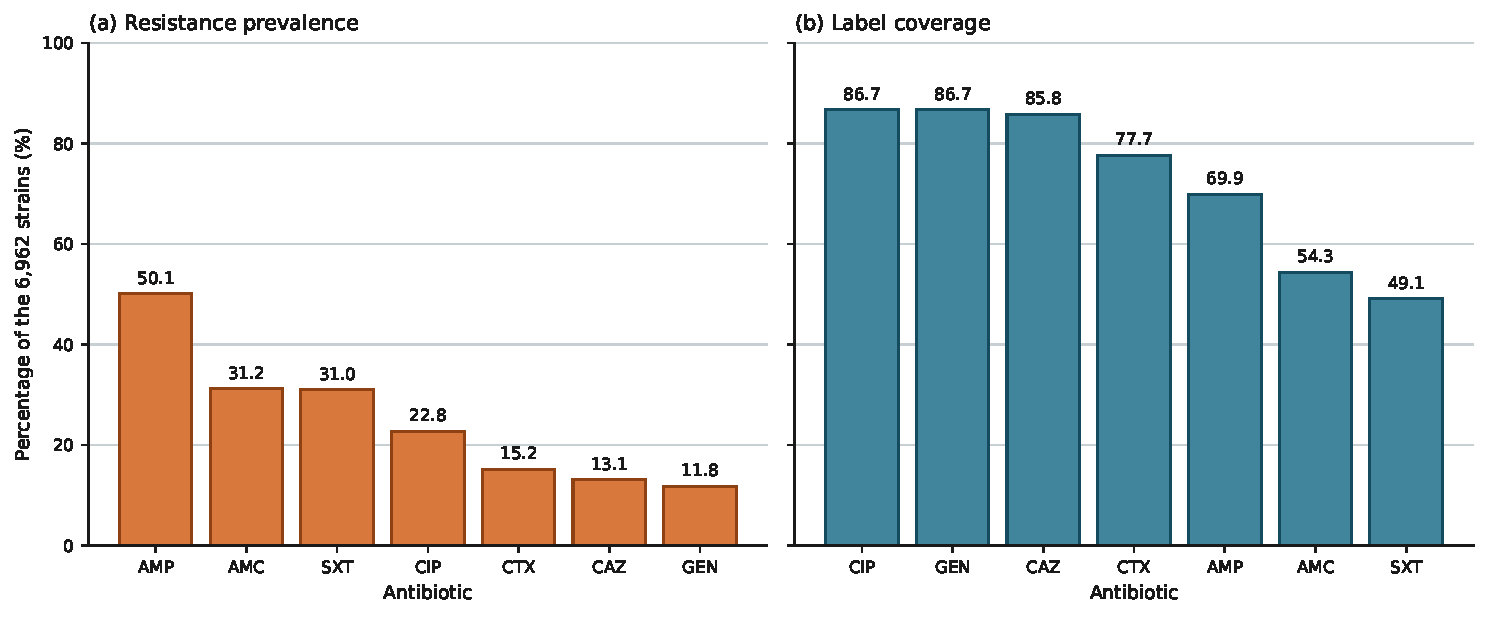
\includegraphics[width=\columnwidth]{fig_label_overview.pdf}
\caption{Resistance prevalence and label coverage for the seven retained
antibiotics. \textbf{(a)} Resistance prevalence, which ranges from 11.8\% for
gentamicin to 50.1\% for ampicillin. \textbf{(b)} Label coverage; no antibiotic
carries a label for more than 86.7\% of the genomes. Both quantities are bounded
above by 100\%.}
\label{fig:label_overview}
\end{figure}

In the cleaned dataset we have built three different genomic views which are
complementary to each other, such that the model is not based on one
representation. The first is a collection of single-nucleotide polymorphism (SNP)
blocks, by gene, of shape $6{,}962 \times 5{,}000 \times 64$, obtained following a
two-step gene filter, both stages of which are fitted on the training partition
alone: a variability filter (kept only genes with at least five
SNPs), which reduced 18{,}975 genes to 13{,}799, and an importance filter (ranked by
gradient-boosting gain), which retained the top 5{,}000 genes. These combined
brought 535{,}439 SNPs to 262{,}225, or about 49\% of the retained variants.
The second view is a gene presence/absence profile with shape
$6{,}962 \times 32{,}441$, which captures resistance genes carried on mobile genetic
elements. The third is a collection of shape $6{,}962 \times 5{,}000 \times 4$
per-gene summaries.

The processed data were split into three parts, a training set of 4{,}872 strains,
a validation set of 1{,}045 strains and a test set of 1{,}045 strains, about a
70/15/15 split. The lineage holdout below assigns whole groups and so lands on
slightly different sizes; Table~\ref{tab:splits} gives the exact figures for all
three. The random split randomly assigns strains, thus related strains can be found
on both sides. The phylogroup-stratified split preserves an equal distribution of
the eight phylogroups in each split. But each phylogroup is present in both the
training and test sets. This test, then, does not measure generalisation to unseen
lineages but simply the effect of the composition of the lineages. The more
challenging question is answered by the sequence-type lineage hold-out split. In
this split, any test strain is not of the same sequence type as one of the training
strains.

TriLens-MoE-Stack is at the center of the system. It has a feature extractor to
extract features from each genomic view and pass them to a separate neural lens.
The SNP blocks are fed into a convolutional network called the Motif Pattern
Encoder, which identifies small and local mutation patterns in each gene. The gene
presence profile goes to the Gene Feature Attention Module, which is a
gated-attention network that focuses on the most informative genes. The per-gene
statistics are sent to a multi-task head called the Cross-Antibiotic Context Module
which provides the ability to share information across similar drugs and helps
drugs with fewer labelled examples. The lenses produce a small summary vector and
seven per-antibiotic scores.

A Mixture-of-Experts Gating Unit is used to concatenate the three representations
into a single 192-length vector. This vector goes through a small network, followed
by a softmax. It calculates the weight for each lens individually for each sample
and each antibiotic. Consequently, the model is able to use various lenses for a
variety of drugs. Simultaneously, the identical gene features feed five base
learners, XGBoost on gene features, LightGBM, Random Forest, Logistic Regression,
and XGBoost on raw features, each of which makes out-of-fold predictions using
five-fold cross-validation. A logistic regression meta-learner combines the neural
probability with the five classical probabilities per antibiotic, and a threshold
transforms the outcome into a resistant or susceptible call. All the seven
antibiotics are forecasted as a multi-label task.

We present the evaluation using four main pillars. Pillar 1 is concerned with
locality. It supports the idea behind the Motif Pattern Encoder. A simple
one-dimensional CNN on the entire pan-genome sequence fails the position-shuffling
test. This demonstrates that positional locality does not hold across the entire
genome. Convolution, however, is more effective within gene blocks. The
architecture is Pillar 2. Pillar 3 is interpretability, taken from the model itself
through its attention and gating weights and contrasted with post-hoc attribution.
The fourth pillar is cross-dataset generalisation, which uses the same methodology
on an independent Giessen \textit{E. coli} collection. We are looking for a measure
of the success of the system, not only in terms of the correct prediction of
resistance, but also one that is appropriate for imbalanced data, primarily
precision-recall AUC supported by clinical error rates, so that we will measure how
much of the accuracy of the system represents genuine mechanism and how much of it
represents population structure.

\subsection{Data Collection}
\label{sec:data}

All findings in this research are based on the construction of the data, and this
section explains the sources of the genomes, how raw variant files were converted
to a format readable by a model, and what was lost during the conversion. We rely
on the \textit{Escherichia coli} genotype and phenotype resource published by
Arcadia Science, which has over seven thousand strains, all of which were sampled
all around the world, and have been lab-tested in terms of their resistance.

This resource has been published in two parts; we use both. The first release
\cite{morin2024ecoli} was a variant calling of the collection against a pan-genome
reference and the variant files were released together with the phenotype table and
strain metadata. The second release \cite{york2025amr} included gene presence and
absence data for all of the genes in all of the strains, as PLINK
\cite{purcell2007plink} binary files. For
credit and clarity, we state which view is from which release and calculate our SNP
views from the first and our gene presence view from the second, not presenting the
combined result as if it came from a single source. There are three reasons we
chose this as a resource rather than building our own collection. The variant calls
were initially quality controlled by the authoring group, effectively eliminating a
significant source of variation between studies. It is part of a pan-genome and not
a single genome, so accessory genes are part of the reference and in \textit{E.
coli} many resistance genes are carried on genes that the strain has obtained from
other sources. And because another group has also published their own analysis of
the exact same strains, we can compare results between ours and theirs later on.

The collection size varies depending on the file you are viewing: the strain
metadata table contains 6,985 rows, the phenotype matrix contains 6,983, and the
presence and absence release lists 7,043 samples. We made no effort to harmonize
these, but retained only the strains which seem everywhere necessary, as described
below.

We created a data pipeline from the raw variant files, filtering by missingness and
frequency, encoding the variants as binary columns in a data matrix, then appended
this to the phenotype table to get a matrix of 6,962 strains by 80,984 features
before settling on this data. We changed direction due to two problems. Our filters
were very crude, based on arbitrary cutoffs that had no biological significance.
More seriously, the features were not structured gene-level: each variant was
simply a column, and there was no connection to the gene it was a part of, and the
entire concept of our proposed model is that mutations within the same gene should
be read jointly. For this reason, we have decided to adopt the curated release
above and rely on it from here on.

\subsection{Data Cleaning}
\label{sec:datacleaning}

This primarily referred to record matching between files and encoding text
phenotypes as numbers. The genomes themselves needed no cleaning, since the variant
calling had already been done and checked.

\subsubsection{Strain Matching Across Files}
Three files were required to match for a strain to be used. The variant file is
indexed by sequencing accession. These are identified in the phenotype file by
genome name. They are mapped via a separate mapping file. An accession was kept if
it was found in the variant file, the mapping file provided a genome name, and that
genome name appeared in the phenotype table. Following this, 6,962 strains remained
and these strains were used for all experiments in this research. We also
incorporated the strain metadata table, 6,821 of which (98.0\%) matched.
Since the metadata is only utilized to work out lineage, the strains without it are
not lost; they simply fall outside of a lineage group.

\subsubsection{Phenotype-to-Label Encoding}
When a test is performed, the result is recorded in the phenotype file as
resistant, intermediate or susceptible and a blank is indicated where no test was
performed. This was transformed to a binary label with 1 for resistant and 0 for
susceptible. In order for our labels to be comparable with the ones produced by the
group that published the dataset, we encoded intermediate results as resistant,
following the same convention as they initially used. There is also a clinical
argument for it: an intermediate result implies that the normal dose will be
insufficient, hence it is safer to call it resistant. One possible consequence of
these early steps is worth remarking on: this step leaves no intermediate category,
which is the reason that categorical agreement collapses to plain accuracy in
Section~\ref{sec:results}.

\subsubsection{Treatment of Untested Strains}
Not all strains were tested against all drugs, and the number of drugs tested
varies a great deal from strain to strain. So, instead of discarding incomplete
lines or inserting guesses, we retained a boolean mask with shape
$6{,}962 \times 7$ that indicates which entries are real. Training loss and all
evaluation metrics are calculated only for the observed entries. Nothing is imputed
anywhere in this research. Table~\ref{tab:labels} displays what remained for us.

\begin{table}[!tb]
\caption{The seven antibiotic labels after cleaning. Coverage is the share of the
6,962 strains tested against that drug; prevalence is the share of those that were
resistant.}
\label{tab:labels}
\centering
\small
\setlength{\tabcolsep}{3pt}
\renewcommand{\arraystretch}{1.05}
\begin{tabular}{|l|r|r|r|r|r|r|}
\hline
\rowcolor{headgrey}
\textbf{Drug} & \textbf{Res.} & \textbf{Susc.} & \textbf{Not tested} & \textbf{Tested} & \textbf{Cov.} & \textbf{Prev.} \\ \hline
AMP & 2,439 & 2,429 & 2,094 & 4,868 & 69.9\% & \textbf{0.501} \\ \hline
CIP & 1,377 & 4,656 &   929 & 6,033 & 86.7\% & 0.228 \\ \hline
AMC & 1,180 & 2,598 & 3,184 & 3,778 & 54.3\% & 0.312 \\ \hline
SXT & 1,060 & 2,358 & 3,544 & 3,418 & \textbf{49.1\%} & 0.310 \\ \hline
GEN &   710 & 5,327 &   925 & 6,037 & 86.7\% & \textbf{0.118} \\ \hline
CTX &   823 & 4,586 & 1,553 & 5,409 & 77.7\% & 0.152 \\ \hline
CAZ &   780 & 5,193 &   989 & 5,973 & 85.8\% & 0.131 \\ \hline
\end{tabular}
\renewcommand{\arraystretch}{1.0}
\vspace{0.4em}

\noindent\footnotesize\textit{Note:} Trimethoprim-sulfamethoxazole has the lowest coverage of
the seven drugs at 49.1\%, and prevalence ranges from 0.501 for ampicillin down to 0.118 for
gentamicin, the two spreads the next paragraph discusses.
\end{table}

There are two items in this table that represent a lot of what happens later.
Overall, almost a twofold variation exists in coverage. Ciprofloxacin and
gentamicin were tested for almost 87\% of strains, but trimethoprim with
sulfamethoxazole for only 49\%, and fewer strains tested means fewer samples
behind a score, which equals a wider confidence interval. It is the chief cause of
some of our intervals in Section~\ref{sec:results} being so much wider than others.

Prevalence ranges more widely: from 0.501 for ampicillin, down to 0.118 for
gentamicin. This is important because the no-skill value of precision recall AUC is
the prevalence: a score of 0.70 on gentamicin, where only 12\% of strains
resist, is a much larger gain over chance than the same score would be on
ampicillin. Four other antibiotics were present in the phenotype file but dropped.
They either were too small to be tested or were so biased that a model would score
well by making too many predictions to one class. The seven we kept cover five
classes of drugs.

\subsection{Data Transformation}
\label{sec:datatransform}

\subsubsection{SNP Matrix Construction}
The variant calls and the gene presence and absence profiles are released in two
different deposits. As a result, the first and second views below are generated
from different source files, instead of one source file. The size of the variant
file is approximately 1.1 gigabytes in compressed VCF. We streamed it just once,
and only retained a variant if two requirements were met. This had to be a
single-nucleotide change, so insertions and deletions were omitted. In addition, it
had to have a minor allele frequency of at least one percent across the collection.
What this left is recorded in Table~\ref{tab:variants}.

\begin{table}[!tb]
\caption{Variant filtering during construction of the SNP matrix.}
\label{tab:variants}
\centering
\small
\setlength{\tabcolsep}{4pt}
\renewcommand{\arraystretch}{1.05}
\begin{tabular}{|l|r|}
\hline
\rowcolor{headgrey}
\textbf{Stage} & \textbf{Variants} \\ \hline
Streamed from the variant file & 2,451,184 \\ \hline
Removed: insertion or deletion &    43,799 \\ \hline
Removed: minor allele frequency below 1\% & 1,871,946 \\ \hline
\rowcolor{oursblue}
\textbf{Kept} & \textbf{535,439} \\ \hline
\end{tabular}
\renewcommand{\arraystretch}{1.0}
\vspace{0.4em}

\noindent\footnotesize\textit{Note:} The 535,439 kept variants are 21.8\% of the 2,451,184
streamed from the variant file, and this is the set that feeds every later step.
\end{table}

The team that constructed this data set reported approximately 2.4 million
variants, and we read 2,451,184, so we knew we were reading it correctly before
building anything on top of it. When the frequency filter was applied alone, 76\%
of the variants were removed, with the majority of them present in just two or
three strains. If a pattern is found in so few strains, then it cannot be expected
that it will hold true for a new strain. So removing these variants was very cheap
for the model.

Genotypes are represented by small integers: 0 is the reference allele, 1, 2 or 3
are the first, second or third alternate. Overall, 83.3\% of the call types
in the data are reference calls and 16.3\% are first alternate; 2.5\%
are second or third alternate, among non-reference calls. We pass these through as
integers and not in separate columns. If the alleles are treated as integers, then
allele 3 is further away from the reference than allele 1. There is no biological
basis to this. Second and third alternate alleles are, however, only 2.5\% of
non-reference calls, about one in forty. One-hot encoding them as separate columns
was therefore not worth the added complexity.

For genotypes missing, they were set to the reference allele in line with the
original authors so that our features match theirs. This is not a neutral choice: a
genotype that failed to call is assumed to match the reference and coverage is
typically lower on plasmids and other mobile elements that are less able to
assemble from the short reads, which is where acquired resistance genes typically
reside. This forms part of our explanation as to why gentamicin is the hardest of
the seven drugs to model. The result is a matrix of $6{,}962 \times 535{,}439$
stored as 8-bit integers, 3.73 gigabytes, which took about two and a half hours to
build on a single consumer GPU.

\subsubsection{The Gene Presence and Absence Matrix}
Release 2 provides the presence of genes in 32,441 pan-genome loci in PLINK binary
format. It took one decision that was not necessarily obvious to make these into a
usable matrix. The numbers stored are 0 and 2. Nothing in the release specifies
which one means the gene is present and the two readings have opposing biology, so
we tried both against something we could test. If non-zero is considered present, the
median gene prevalence across loci is 0.966 and the average strain then carries about
28,700 of the 32,441 genes. If zero is coded as present, the median gene prevalence is
0.034 and the average strain carries 3,709 genes (range 2,141 to 8,333). The two
statistics are reported side by side and not derived from one another: the median is
taken over loci and the count over strains, and because the distribution of gene
prevalence is strongly skewed the count is not the median multiplied by 32,441. An
\textit{E. coli} genome contains about 4-5 thousand genes, limiting the reading to
the second one, which is the one we use.

We register this check because the incorrect option need not have thrown any error.
The model would have learned as usual with its gene matrix inverted and since this
view has a lot of weight in our final model, everything further down it would have
been incorrect in a non-obvious way. The per-strain gene count is a sanity check
and is now done automatically on every new matrix build. There are 6,962 strains of
which 6,949 are found in the PLINK sample list. The other 13 (0.19\%) do not
have a record of gene presence. In the default policy of the pipeline these rows
are not dropped or masked, instead remaining as an all-zero gene-presence vector,
meaning that Lens B interprets them as a strain with non-detected genes instead of
excising them from the dataset. This conflates a missing record with a genuinely
empty accessory genome, which is not the same thing, and the correct handling is to
extend the label mask of Section~\ref{sec:datacleaning} to cover the gene-presence
view for these rows. At 0.19\% of the collection, and with the 13 strains distributed
across partitions in proportion, the effect on any figure reported here is below the
resolution of the intervals in Section~\ref{sec:statanalysis}, so we record the defect
rather than reporting a corrected set of results.

\subsubsection{Per-Gene Statistics}
The third view summarizes each gene with four values calculated from its SNPs: mean
value of the alleles, variance of the alleles, number of positions that do not
match the reference, and maximum value of the alleles. It is a very broad
perspective, and it cannot tell where a mutation is occurring in a gene. It does
offer stability and compactness though. It also provides a brief and reliable
gene-level view of variation which complements the other two views.

Each of these four statistics is on a different scale. Therefore, each one is
adjusted in order to have zero mean and unit variance before it gets to the third
lens. Only the training partition is used to calculate the means and standard
deviations. They are then applied unchanged to the validation and test partitions.
This means that no test genome impacts the scaling.

\subsubsection{Lineage Encoding}
Bacterial populations are structured in lineages and strains within a lineage are
likely to share their genetic background and resistance pattern. In order to
determine if our model was using lineage or mechanism we first had to determine the
lineage of each strain, which the data set did not explicitly give us, but we worked
it out ourselves. The phylogroup, in the sense of the Clermont typing scheme
\cite{clermont2013phylotyping}, was not provided directly. We have developed it in
two steps. An explicit phylogroup assignment, if any, is taken from the typing field
in the strain metadata. In the absence of such information, the multi-locus
sequence type and mapping to a phylogroup were done with the help of a look-up table
of 57 common multi-locus sequence types. There is no record of the origin of this
particular table in the original notebooks used for data preparation. No citation or
generation script is recorded with it and it is reported here as an undocumented
lookup, not as a part of a published scheme. It is therefore weaker evidence than a
direct assignment would be: the established route is to call the phylogroup from the
genome itself with an \textit{in silico} implementation of the Clermont quadruplex,
such as ClermonTyping \cite{beghain2018clermontyping}, and a study that depends on
the phylogroup as more than a coarse covariate should do so. If a strain is found
that cannot be fixed by either route it is marked Unknown.
Table~\ref{tab:phylogroups} gives the result.

\begin{table}[!tb]
\caption{Phylogroup composition of the 6,962 strains.}
\label{tab:phylogroups}
\centering
\small
\setlength{\tabcolsep}{4pt}
\renewcommand{\arraystretch}{1.05}
\begin{tabular}{|l|r|r|}
\hline
\rowcolor{headgrey}
\textbf{Phylogroup} & \textbf{Strains} & \textbf{Share} \\ \hline
B2      & 3,542 & \textbf{50.9\%} \\ \hline
Unknown & 1,697 & \textbf{24.4\%} \\ \hline
D       &   723 & 10.4\% \\ \hline
A       &   317 &  4.6\% \\ \hline
F       &   307 &  4.4\% \\ \hline
B1      &   258 &  3.7\% \\ \hline
C       &   114 &  1.6\% \\ \hline
E       & \textbf{4} &  0.06\% \\ \hline
\end{tabular}
\renewcommand{\arraystretch}{1.0}
\vspace{0.4em}

\noindent\footnotesize\textit{Note:} B2 alone is 50.9\% of the collection, 24.4\% of strains
have no assigned phylogroup, and phylogroup E has only 4 members, too few for any per-group
estimate; these are the three limits the next paragraph discusses.
\end{table}

There are, however, three features of this table which restrict what can be read
from it; we should like to mention them here rather than have them pointed out
later. B2 is slightly more than half the collection, so the analysis of splitting
the collection by phylogroup is a majority analysis of B2 vs.\ the remainder of the
collection. There is little use for a per-group estimate of the diversity of the
Unknown group because almost a quarter of strains could not be assigned to any
group, and phylogroup E has a small number of members (four), which is too small to
make any estimate meaningful. For this reason we consider the phylogroup as a broad
category and not anything else. It is encoded as an eight-way one-hot vector and
used as a covariate and as a grouping variable. We do not consider it as a fine
description of ancestry.

\subsection{Data Integration}

We had two checks before training. The three feature matrices were of different
files. They were also produced in various stages. We therefore made sure that they
had the same strains in the same order. We also verified that they were using the
same names of genes. The first confirmed that the ordering of all 6,962 strain
identifiers is identical in all views; otherwise, one genome's SNPs would be paired
with another genome's genes.

The latter one discovered a real challenge. None of the genes were found in common
when the gene identifiers in the SNP views were compared to the presence and
absence view, because the PLINK reader had created its own placeholder names for the
genes and not read the actual gene identifiers from the annotation file. Once the
reader was corrected, all 5,000 genes chosen for the SNP views were found in the
32,441-gene catalogue, a 100\% overlap. Nothing would have failed visibly had
this check not been run. The model would have received views labelled with the wrong
gene names, and the gene-level reading would have been comparing labels with no
meaning against one another. Both the checks are now programmed as a fixed step
prior to any training run.

\subsection{Data Reduction}

There are 535,439 features for 6,962 strains (some 77 candidate features for each
sample). So, it was not an optimisation to reduce the feature space. It was
necessary for modelling. The features were reduced at the gene level rather than at
the individual-variant level as the model operates at the gene level. Lastly, only
the genes that survived the two filters were retained. If a gene has fewer variable
positions, we cannot support a within-gene pattern, which is what our first view is
designed to find; thus the variability filter retains a gene if it has five or more
SNPs within the training partition of the split being fitted. After this step, 13,799
of the 18,975 genes in the matrix remain on the random split. These genes are then sorted by importance in the gradient boosting
model \cite{chen2016xgboost} using the importance filter. That model is trained
separately for each of the seven antibiotics. First, we filtered each set of SNPs
with a chi-squared pre-filter and kept the top 50,000 per drug, and trained a single
XGBoost model for each antibiotic on its respective chi-squared filtered subset,
calculating each gene's cumulative gain for each model. The final importance score
for each gene is the sum of the per-antibiotic importance over all seven models, and
the 5,000 most important (highest summed) genes are retained.

Both of these filters were fitted solely on the training partition, and refitted from
scratch for each of the three splits. This is quite
easy to forget, and quite hard to do well: had the test labels been visible during
ranking, they would have changed what features exist in the first place, and each
score in Section~\ref{sec:results} would then have been overoptimistic by an unknown
amount.

One earlier stage does not meet that standard, and we state it rather than leave it to
be inferred. The variant-level filters of Section~\ref{sec:datatransform}, namely the
removal of insertions and deletions and of variants with a minor allele frequency below
one percent, were computed once over the whole collection, before any split existed. They
use no phenotype label, so they cannot transmit outcome information, but they do let the
allele frequencies of the test strains influence which columns are available to the
model. We regard this as a weaker form of leakage than a label-aware filter would be, and
we did not repeat it per split because doing so would give the three splits different
feature spaces and make their scores incomparable, which is the comparison the paper is
built on. Figure~\ref{fig:gene_feature_space} shows how much the gene feature space is
reduced by the two gene-level filters used above.

\begin{figure}[!tb]
\centering
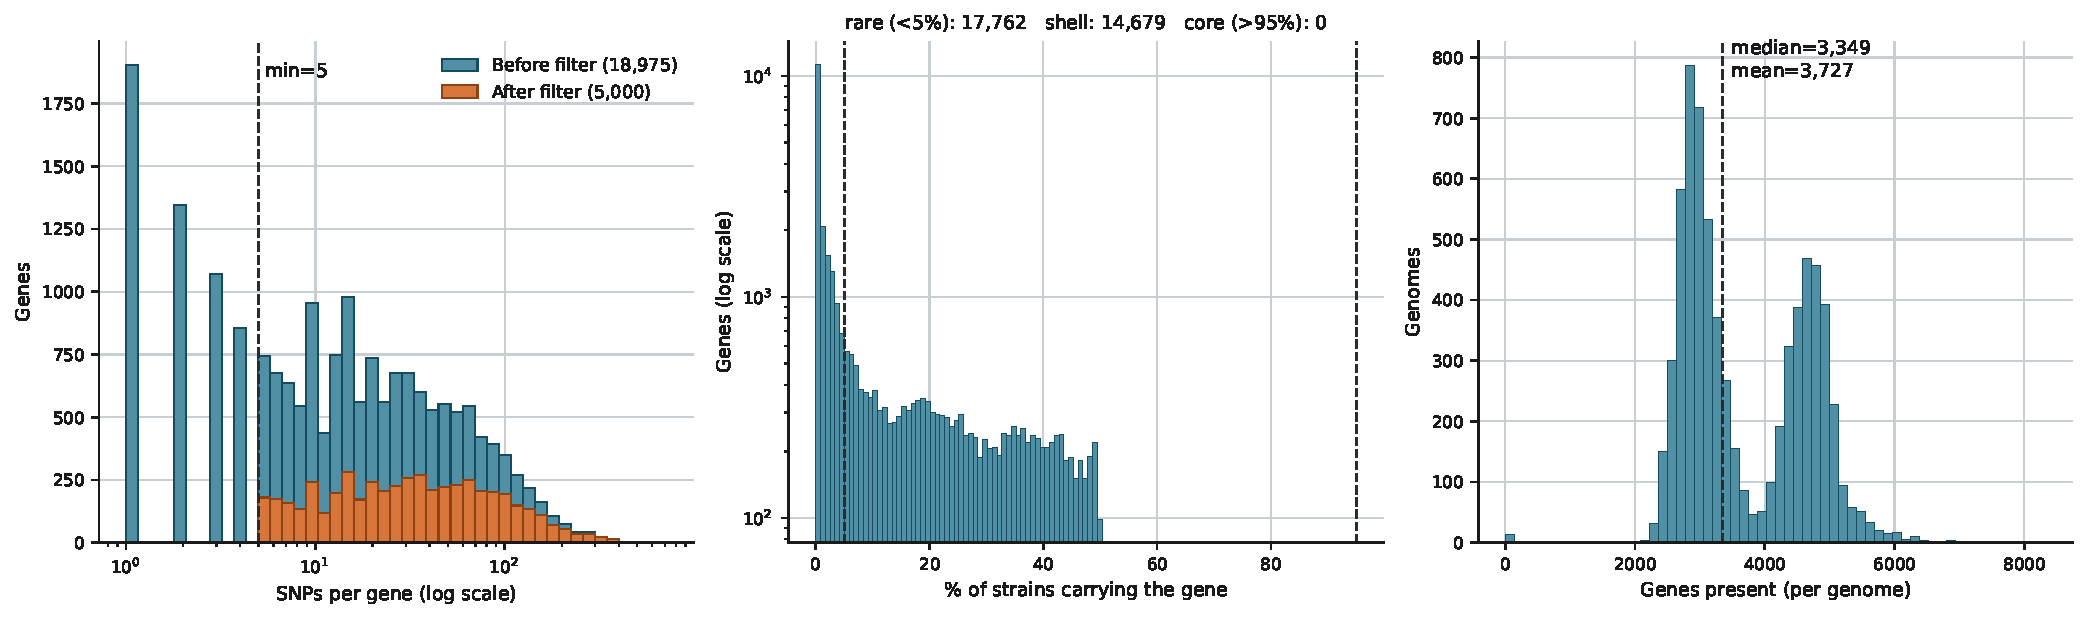
\includegraphics[width=\columnwidth]{fig_gene_feature_space.pdf}
\caption{The gene feature space before and after filtering. \textbf{(a)} SNPs per
gene across the 18{,}975 genes of the SNP view, before and after the variability and
importance filters cut them to 5{,}000. \textbf{(b)} and \textbf{(c)} the separate
32{,}441-gene presence and absence catalogue, which is mostly rare genes ---
17{,}762 are carried by under 5\% of strains and none by more than 95\%, and a
typical genome holds a median of 3{,}349 of them against a mean of 3{,}709.}
\label{fig:gene_feature_space}
\end{figure}

After filtering, 5,000 genes remain. These genes contain 262,225 SNPs. This
corresponds to approximately 49.0\% of the 535,439 variants retained after the
variant-level filters, and to about 10.7\% of the 2,451,184 originally streamed. These genes differ
widely in size: the smallest carries 5 SNPs, the median 32, the mean 52, and the
largest 717. That distribution fed one last decision. Our first view reads each gene
as a fixed length block, which we set to 64 positions. Approximately 28\% of the
selected genes are longer than 64 SNPs and are truncated, the remaining genes are
padded with zeros and masked with zeros, so the padding does not contribute. A gene
block has an average of 35 positions out of 64 that are occupied by real positions.
Most genes would waste memory if the block were too long, while a shorter block
would cause the median gene to be cut.

\subsection{The Three Evaluation Splits}
\label{subsec:splits}

The splits determine what a score measures, because of which we give a detailed
account of how we split the data. Approximately 15\% of each split is for
testing, another 15\% of each split is for validation, and approximately 70
percent is for training. The test set is never used in the model selection or
tuning; it is not touched until the final evaluation, and every split has been
performed with the same fixed random seed (42), which means that any number reported
in this research can be exactly re-generated by running the same code. We
constructed three splits and they address three questions.

The random split assigns strains via shuffling, stratified on the ampicillin label
to achieve class balance across the three sets. This results in a training set of
4,872 strains, a validation set of 1,045 and a test set of 1,045. It is the normal
setting, and the one that is used in the majority of published work; the related
strains can fall on both sides, and do. The partition sizes remain the same but the
partition balancing takes into account the eight-way phylogroup assignment, each
lineage group being represented in each of the three sets in the same proportion as
it would be in the collection as a whole. This does not control class balance. The
proportional guarantee is meaningful for the six larger groups; for phylogroup E,
which has four members in the entire collection, a 70/15/15 allocation places at most
one strain in the test partition, so that group is present in the split by
construction but carries no evidential weight.

We just want to clarify what this second split is, as it can be very easily
inflated. It is a stratified split, as opposed to a holdout. By design, every
phylogroup appears on both sides so it is not testing how the model performs on a
lineage it has never seen before. What it tests is the extent to which the result is
influenced by the choice of stratification variable. This is a weaker question than
the one we wished to answer.

The train/test split answering that more stringent question is the sequence-type
lineage holdout, and is the one upon which the central result of this research is
built, so we will describe its construction in full. Strains each have a
multi-locus sequence type, a generic label in bacterial genomics that clusters
strains based on shared descent in the recent past and is much more specific than
phylogroup. We did not call sequence types ourselves. They were taken from the
sequence-type field of the strain metadata distributed with the primary collection
\cite{morin2024ecoli}, which reports the seven-locus Achtman scheme for
\textit{E. coli}. Because the metadata table and the variant matrix are ordered
differently, the join was made on the sequencing accession carried by both, and not
on the position or row of a strain in either table; that distinction matters, because
joining by row silently mislabels the lineage of every strain and would invalidate the
split this paper is built on. The join recovered a sequence type for the large
majority of the collection. Two consequences follow from taking the types as given.
The scheme resolves clones but not clonal complexes, so two sequence types that are
single-locus variants of one another, as several members of the ST131 complex are,
can still be separated across partitions, and the holdout is therefore a lower bound
on lineage novelty rather than a guarantee of it. And any error in the upstream typing
propagates into our split without our being able to detect it.

Two rules were set prior to examining any result. In the absence of a sequence type,
any strain was assigned to training as an unlabelled group cannot be held out
safely. If the number of sequences in a collection type was more than five percent,
then it was also put in training. The other rule is equally important. Type 73
represents approximately an eighth of the entire dataset. If that clone has a
relatively large number of different strains found in the test set, the test will
mostly be measuring this particular clone. This does not measure how well the model
will work on novel lineages. The rest of the sequence types were then allocated
whole to training, validation or test by a seeded permutation walk which
successively adds groups until the desired proportion of genomes in each partition
is reached. Figure~\ref{fig:st_distribution} shows the size distribution these rules
had to work around.

\begin{figure}[!tb]
\centering
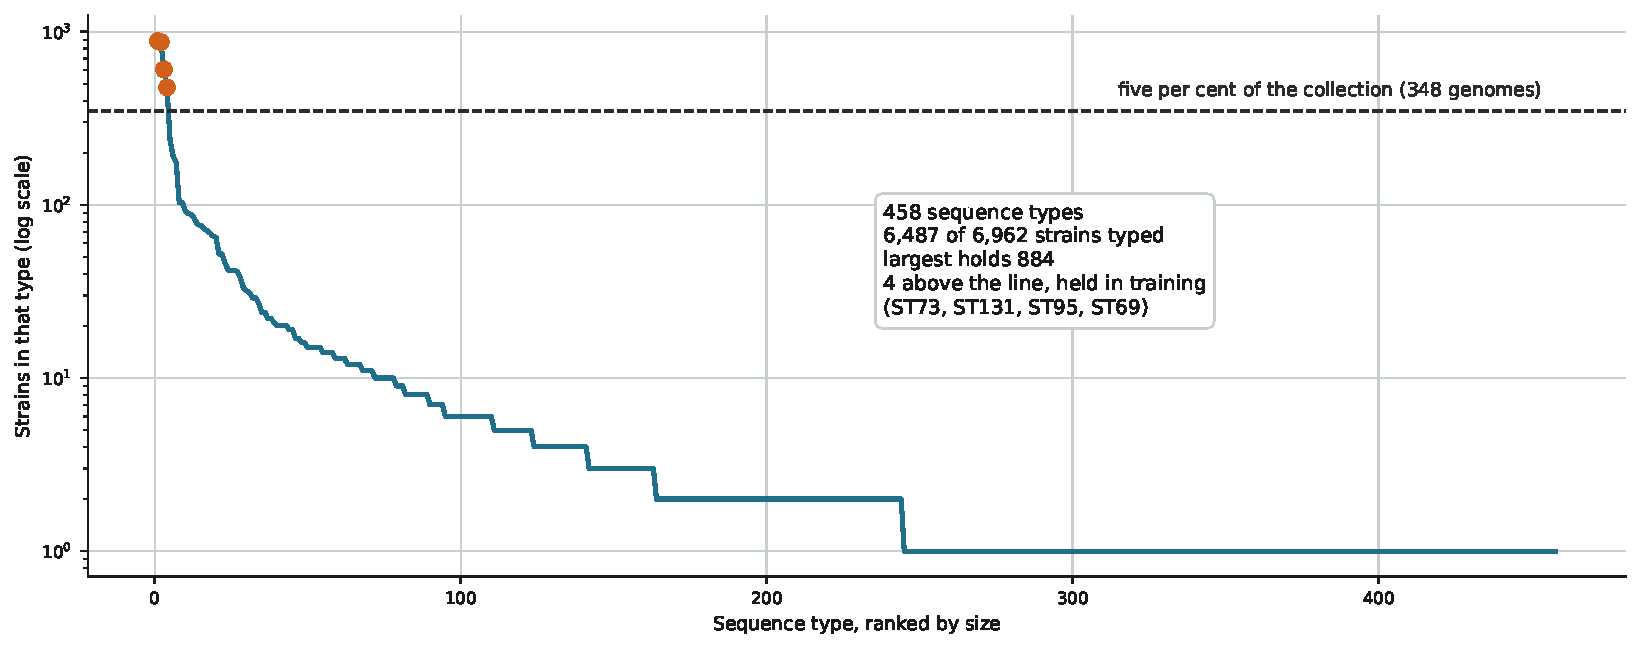
\includegraphics[width=\columnwidth]{fig_st_distribution.pdf}
\caption{The 458 sequence types, ranked by size. A few are very large and most are
very small. The largest holds 884 strains, nearly one genome in eight, and four
types sit above five percent of the typed collection. Those four are placed in
training, so that no test set can be dominated by a single clone.}
\label{fig:st_distribution}
\end{figure}

We kept whole groups in the same partition. Owing to this, there are no ideal
percentages of the split. A chance division would appear less lopsided. This effect
is reflected in our data split as well. The holdout uses a training set of 4,836
strains, a validation set of 1,081 and a test set of 1,045. No sequence type was
observed to be present in more than one partition, as opposed to assuming this. The
same point of method is used for all three splits. The 5,000 gene selection
mentioned earlier under Data Reduction is re-fitted on each split's training
partition instead of being computed only once and used for each split. The
definition of the pipeline used an earlier version that leaked information between
splits, which was fixed prior to any results in this research. Refitting per split
indicates that each split generates its own ranking of informative genes. Notably,
the holdout's gene set overlaps the random split's by less than half, indicating
that the resistance signal is not located in a few genes but in many genes that are
partly interchangeable.

\begin{table}[!tb]
\caption{The three evaluation splits and the partition sizes they produce. Only the
third assigns whole groups, which is why its sizes are not round.}
\label{tab:splits}
\centering
\footnotesize
\setlength{\tabcolsep}{3pt}
\renewcommand{\arraystretch}{1.05}
\begin{tabular}{|l|l|r|r|r|}
\hline
\rowcolor{headgrey}
\textbf{Split} & \textbf{Balanced on} & \textbf{Train} & \textbf{Val} & \textbf{Test} \\ \hline
Random & Ampicillin label & 4{,}872 & 1{,}045 & 1{,}045 \\ \hline
Phylogroup-stratified & Eight-way phylogroup & 4{,}872 & 1{,}045 & 1{,}045 \\ \hline
Sequence-type holdout & Whole sequence types & 4{,}836 & 1{,}081 & 1{,}045 \\ \hline
\end{tabular}
\renewcommand{\arraystretch}{1.0}
\end{table}

For each split we also record the number of labelled strains and the resistance
prevalence in each partition, per antibiotic. The lower bound of precision recall
AUC will be determined by prevalence, meaning that a lower prevalence will result in
a lower score even if the model is equally good. The effects are greatest for the
holdout, as forcing the largest clones into training causes a shift in prevalence
downwards for all of the antibiotics. Reporting the prevalence with the score
enables a reader to distinguish a drop because of a tougher test set from a drop
because of a lower floor. Figure~\ref{fig:split_prevalence_shift} shows how large
that shift is for each split.

\begin{figure}[!tb]
\centering
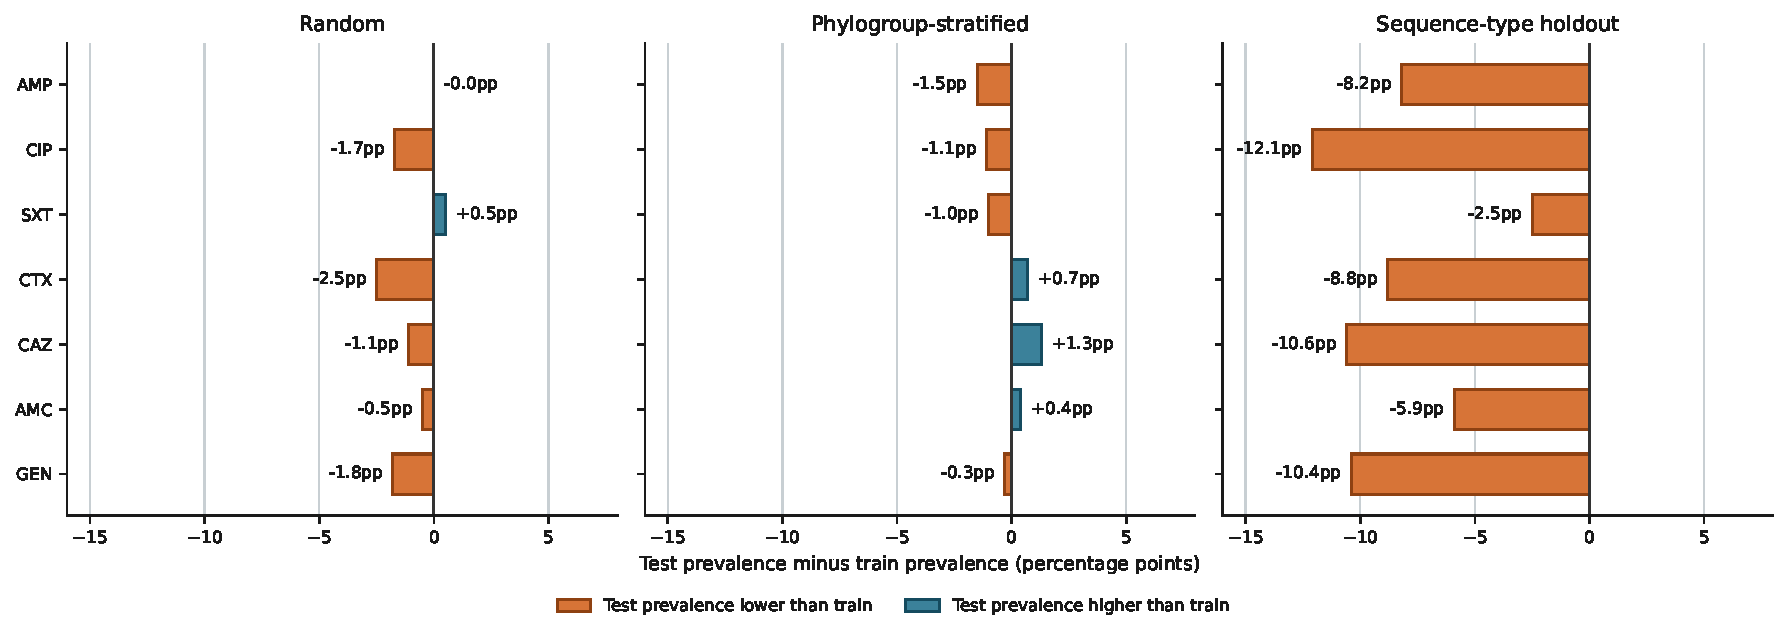
\includegraphics[width=\columnwidth]{fig_split_prevalence_shift.pdf}
\caption{Resistance prevalence in the test partition minus the training partition,
in percentage points, per antibiotic and per split. The random and
phylogroup-stratified splits stay within 2.5 points and move in both directions. The
sequence-type holdout moves downwards for every antibiotic, by 2.5 to 12.1 points,
and since the no-skill floor of precision recall AUC is the prevalence itself, part
of the drop reported later follows from this shift rather than from the model.}
\label{fig:split_prevalence_shift}
\end{figure}

Now combining the three genomic views with the encoding of the phylogroup, the
labels and their mask provides the six arrays that are actually passed to the model,
which are contained in Table~\ref{tab:views}.

\begin{table}[!tb]
\caption{Arrays produced by the preprocessing pipeline: four feature
representations, followed by the label matrix and its mask.}
\label{tab:views}
\centering
\footnotesize
\setlength{\tabcolsep}{2pt}
\renewcommand{\arraystretch}{1.05}
\begin{tabular}{|l|l|>{\raggedright\arraybackslash}p{2.0cm}|}
\hline
\rowcolor{headgrey}
\textbf{Representation} & \textbf{Shape} & \textbf{What it captures} \\ \hline
SNP blocks by gene    & $6{,}962 \times 5{,}000 \times 64$ & mutation patterns inside genes \\ \hline
Gene presence/absence & $6{,}962 \times 32{,}441$          & genes acquired from elsewhere \\ \hline
Per-gene statistics   & $6{,}962 \times 5{,}000 \times 4$  & coarse gene-level variation \\ \hline
Phylogroup one-hot    & $6{,}962 \times 8$                 & broad lineage \\ \hline
Labels                & $6{,}962 \times 7$                 & resistant or susceptible \\ \hline
Label mask            & $6{,}962 \times 7$                 & which labels were measured \\ \hline
\end{tabular}
\renewcommand{\arraystretch}{1.0}
\end{table}

Two characteristics of this data set set the stage for everything that follows. It
is broad and short: there are still far more features than strains even after
dimensionality reduction, so the design favors gradient boosting over a large
network. And it is patchy: antibiotic coverage ranges from 49 to 87\%
according to drug while prevalence ranges from 12 to 50\%, meaning no
averaged score across the seven antibiotics serves it well; hence each result in
Section~\ref{sec:results} is reported per drug, as well as on average.

\subsection{The External Giessen Collection}

A single collection does not provide an answer to the question of whether or not an
approach travels. We use a second, independent set of \textit{E. coli} genomes that
were collected at the University of Giessen and published by Ren et al.\
\cite{Ren2022}. Isolates were from human and animal clinical specimens and
susceptibility was done by automated testing and interpreted according to European
Committee on Antimicrobial Susceptibility Testing (EUCAST)
breakpoints \cite{eucast_breakpoints}. Ren et al.\ report 987 Giessen isolates in
total; the subset we use is the 809 that carry a complete result for all four of the
antibiotics shared with our panel, which is the same 809 used by Siddiqui and
Tarannum \cite{siddiqui2025amrensemble}, prior work of one of the present authors. Those 809 strains are described by 60,936 SNP
positions each. Its composition is shown in Table~\ref{tab:giessen}.

\begin{table}[!tb]
\caption{Composition of the external Giessen dataset.}
\label{tab:giessen}
\centering
\small
\setlength{\tabcolsep}{4pt}
\renewcommand{\arraystretch}{1.05}
\begin{tabular}{|l|r|r|r|}
\hline
\rowcolor{headgrey}
\textbf{Antibiotic} & \textbf{Resistant} & \textbf{Susceptible} & \textbf{Prevalence} \\ \hline
CIP & 366 & 443 & 0.452 \\ \hline
CTX & 358 & 451 & 0.443 \\ \hline
CAZ & 276 & 533 & 0.341 \\ \hline
GEN & 188 & 621 & 0.232 \\ \hline
\end{tabular}
\renewcommand{\arraystretch}{1.0}
\end{table}

There are two disparities with the Arcadia data that influence its use. The first
one is the reference. In Giessen variants are listed in order of a single reference
genome (columns are ordered along the chromosome) while Arcadia uses a pan-genome
(the ordering of the columns has no meaning). This difference is not an
inconvenience: it makes the locality test possible because we have one set of data
for which locality should matter, and one set for which it should not. The second is
the two feature spaces have no overlap. The model trained on Arcadia cannot be used
at Giessen, since there is no shared feature vector, so anything we do across the two
collections must be a comparison of methods.

Also, there is a difference in the label names. The Giessen phenotypes are
interpreted against the EUCAST breakpoints, and the Arcadia phenotypes are
interpreted according to a different standard. Breakpoint differences between the two
also exist for the same drug, and this could contribute to performance differences
between collections, and not only to the model. We are unable to separate the two
effects with the data available and designate it as a limitation for any
cross-collection comparison. This dataset consists of 809 strains with results for
all four types of drugs, unlike Arcadia where some of the labels are missing, so
masking is not necessary. The numbers were randomly split by ciprofloxacin into 647
for training, 81 for validation and 81 for testing. The test partition is small and
that is why the Giessen confidence intervals are wider than those for Arcadia.

% =====================================================================
\section{The TriLens-MoE-Stack Architecture}
\label{sec:architecture}
% =====================================================================

The proposed model TriLens-MoE-Stack is a hybrid architecture in which a stacking
meta-learner is used to join classical machine learning models with neural lenses.
The name illustrates the design: \textit{TriLens} comes from the three genome
perspectives the model uses. \textit{MoE} stands for Mixture of Experts, where a
gate determines how much each view should contribute. \textit{Stack} refers to how
the outputs of multiple classical models are combined to produce the final
prediction. The concept is that a bacterial genome can be defined in more than a
single manner and no single definition is complete by itself. A mutation-based
stance will lose a resistance gene that came into the plasmid, since that gene is
not a mutation, it is only there. A point mutation in a target enzyme is not
detectable by the gene presence view. This is because the gene is present in both
resistant and susceptible strains. The only difference is a single nucleotide
change. Instead of selecting between these views, our design incorporates all three
and defers to the model to determine the importance of each view for each
antibiotic.

This system has three components and the entire architecture is presented in
Fig.~\ref{fig:trilens-overall}. To begin with, the three genomic views are
processed by a neural feature extractor that uses three specialised lenses and
combines them with a mixture-of-experts gate. We then use the gene features to train
five classical base learners. They make leak-free out-of-fold predictions. Third, a
logistic-regression meta-learner combines the neural and the classical predictions
into a single per-antibiotic prediction.

In the model, each component generates a raw score $z$, whose value may be any real
number, and the score is converted into a probability in the range 0 to 1 with the
help of the logistic sigmoid function,
\begin{equation}
\sigma(z) = \frac{1}{1 + \exp(-z)},
\label{eq:sigmoid}
\end{equation}

\begin{figure*}[!tb]
\centering
\resizebox{0.92\textwidth}{!}{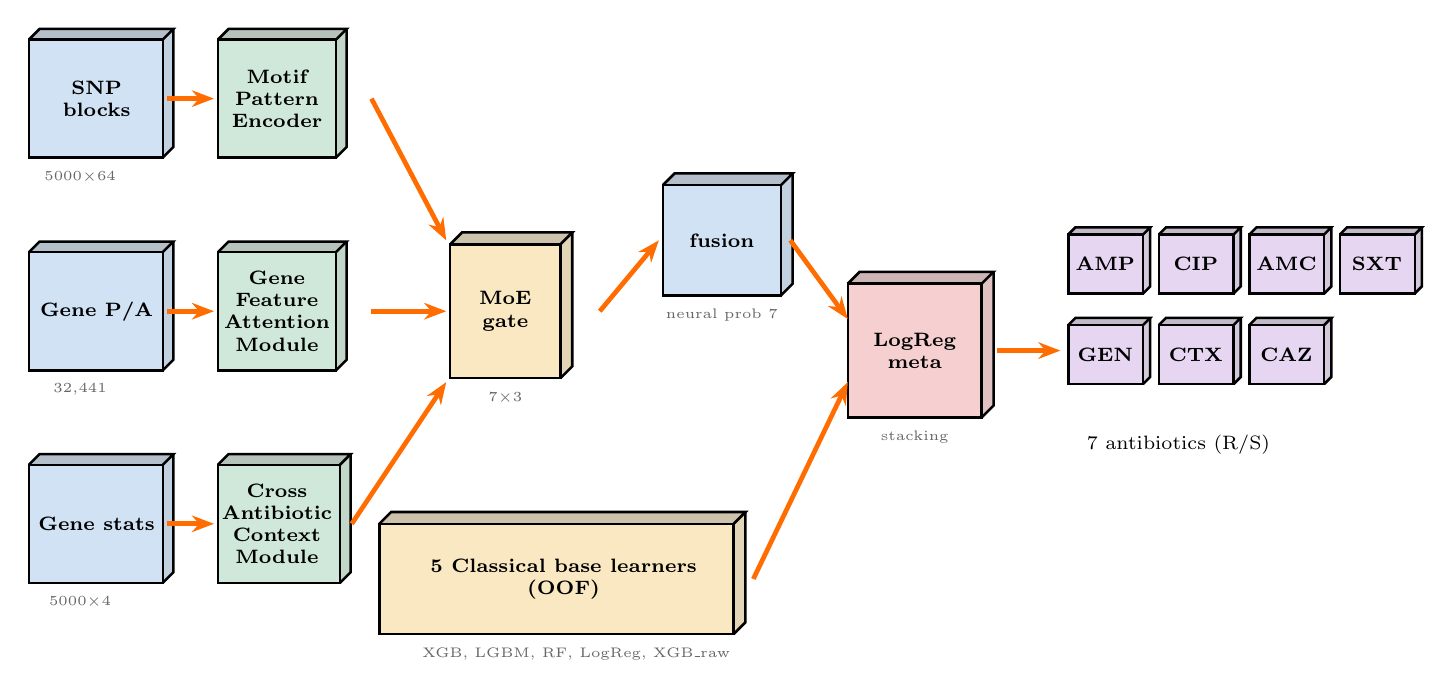
\begin{tikzpicture}[font=\sffamily,>=Stealth,
 ar/.style={-{Stealth[length=2.8mm]},line width=0.6mm,draw=orange!85!red}]
\blk{0}{2.7}{1.7}{1.5}{0.45}{cin}
\node[font=\scriptsize\bfseries,align=center] at (0.86,2.7) {SNP\\blocks};
\node[below,font=\tiny,text=black!60,align=center] at (0.65,1.9) {$5000{\times}64$};
\draw[ar] (1.75,2.7)--(2.35,2.7);
\blk{2.4}{2.7}{1.5}{1.5}{0.45}{cexp}
\node[font=\scriptsize\bfseries,align=center] at (3.15,2.7) {Motif\\Pattern\\Encoder};
\draw[ar] (4.35,2.7)--(5.3,0.9);
\blk{0}{0.0}{1.7}{1.5}{0.45}{cin}
\node[font=\scriptsize\bfseries,align=center] at (0.86,0.0) {Gene P/A};
\node[below,font=\tiny,text=black!60,align=center] at (0.65,-0.8) {$32{,}441$};
\draw[ar] (1.75,0.0)--(2.35,0.0);
\blk{2.4}{0.0}{1.5}{1.5}{0.45}{cexp}
\node[font=\scriptsize\bfseries,align=center] at (3.15,0.0) {Gene\\Feature\\Attention\\Module};
\draw[ar] (4.35,0.0)--(5.3,0);
\blk{0}{-2.7}{1.7}{1.5}{0.45}{cin}
\node[font=\scriptsize\bfseries,align=center] at (0.86,-2.7) {Gene stats};
\node[below,font=\tiny,text=black!60,align=center] at (0.65,-3.5) {$5000{\times}4$};
\draw[ar] (1.75,-2.7)--(2.35,-2.7);
\blk{2.4}{-2.7}{1.55}{1.5}{0.45}{cexp}
\node[font=\scriptsize\bfseries,align=center] at (3.15,-2.7) {Cross\\Antibiotic\\Context\\Module};
\draw[ar] (4.1,-2.7)--(5.3,-0.9);
\blk{5.35}{0}{1.4}{1.7}{0.5}{cgate}
\node[font=\scriptsize\bfseries,align=center] at (6.05,0) {MoE\\gate};
\node[below,font=\tiny,text=black!60,align=center] at (6.05,-0.9) {$7{\times}3$};
\draw[ar] (7.25,0)--(8.0,0.9);
\blk{8.05}{0.9}{1.5}{1.4}{0.5}{cin}
\node[font=\scriptsize\bfseries,align=center] at (8.8,0.9) {fusion};
\node[below,font=\tiny,text=black!60,align=center] at (8.8,0.15) {neural prob 7};
\blk{4.45}{-3.4}{4.5}{1.4}{0.5}{cgate}
\node[font=\scriptsize\bfseries,align=center] at (6.79,-3.4) {5 Classical base learners\\(OOF)};
\node[below,font=\tiny,text=black!60,align=center] at (6.95,-4.15) {XGB, LGBM, RF, LogReg, XGB\_raw};
\blk{10.4}{-0.5}{1.7}{1.7}{0.5}{cmeta}
\node[font=\scriptsize\bfseries,align=center] at (11.25,-0.5) {LogReg\\meta};
\node[below,font=\tiny,text=black!60,align=center] at (11.25,-1.4) {stacking};
\draw[ar] (9.67,0.9)--(10.4,-0.1);
\draw[ar] (9.2,-3.4)--(10.4,-0.9);
\draw[ar] (12.3,-0.5)--(13.1,-0.5);
\blk{13.2}{0.6}{0.95}{0.75}{0.3}{cout}
\node[font=\scriptsize\bfseries,align=center] at (13.67,0.6) {AMP};
\blk{14.35}{0.6}{0.95}{0.75}{0.3}{cout}
\node[font=\scriptsize\bfseries,align=center] at (14.82,0.6) {CIP};
\blk{15.5}{0.6}{0.95}{0.75}{0.3}{cout}
\node[font=\scriptsize\bfseries,align=center] at (15.97,0.6) {AMC};
\blk{16.65}{0.6}{0.95}{0.75}{0.3}{cout}
\node[font=\scriptsize\bfseries,align=center] at (17.12,0.6) {SXT};
\blk{13.2}{-0.55}{0.95}{0.75}{0.3}{cout}
\node[font=\scriptsize\bfseries,align=center] at (13.67,-0.55) {GEN};
\blk{14.35}{-0.55}{0.95}{0.75}{0.3}{cout}
\node[font=\scriptsize\bfseries,align=center] at (14.82,-0.55) {CTX};
\blk{15.5}{-0.55}{0.95}{0.75}{0.3}{cout}
\node[font=\scriptsize\bfseries,align=center] at (15.97,-0.55) {CAZ};
\node[font=\scriptsize,align=center] at (14.6,-1.7) {7 antibiotics (R/S)};
\end{tikzpicture}
}
\caption{Overall dataflow of TriLens-MoE-Stack: three genomic views feed three
lenses, which the mixture-of-experts gate fuses before stacking with five classical
base learners.}
\label{fig:trilens-overall}
\end{figure*}

\subsection{Rationale for the Hybrid Design}
\label{subsec:hybrid}

Combining neural and classical models is one of the most crucial design decisions.
We use both instead of one deep neural network. An apparent solution in the
contemporary world would be an end-to-end trained network. We have experimented with
that, and it was not very good, but the reason is in the form of the data, and not
in anything wrong with the network. Deep learning works best in situations where the
number of training examples is significantly larger than the number of input
features; our scenario is the opposite with only 6{,}962 labelled strains and
hundreds of thousands of candidate genomic features. The training data can also be
memorised in a model that can utilise all this information. Even with this number of
samples, dropout cannot completely avoid that issue.

Gradient boosted trees are much more suited for this type of data. For a feature
containing no signal, the split predictor will just never consider that feature for
a split, and it requires far fewer examples to train a stable model. The classical
arm, then, is not a fallback or a leftover baseline, it is a load-bearing part of
the final design. Meanwhile, classical models regard each feature as an independent
column: they cannot encode the idea that various mutations near each other within a
single gene function as one pattern, nor that resistance to one cephalosporin says
something about another. Those are precisely the types of tasks a neural network
excels at, meaning that the design pairs both, with each arm addressing the other's
weakness. Section~\ref{sec:results} provides the proof: on the random split the
neural arm alone hits 0.781 while the combination 0.849, and under the lineage
holdout the classical learners alone score 0.628 while the full model gets 0.634,
but the neural arm yields only 0.472.

\subsection{Classical Base Learners}

The classical arm comprised five base learners: the XGBoost on the gene-aggregated
features (XGB\_gene), LightGBM, Random Forest, Logistic Regression and a second
XGBoost on a chi-squared-prefiltered raw feature matrix (XGB\_raw). These five are
trained in an independent five fold stacking pipeline, and the five out of fold
predictions are provided to the meta-learner of Section~\ref{subsec:metalearner}.
Each of the five on their own is presented as a baseline for the proposed model in
Section~\ref{sec:results}.

Five models might appear to be more than is needed so it is worth explaining why.
Only when models of an ensemble commit a variety of errors does the ensemble work.
When two models commit similar errors, their combination does not give much
advantage. It averages just two similar false forecasts. We thus selected five
learners who fail in various manners. Both XGBoost and LightGBM are gradient
boosting methods, but they expand their trees in different ways, thus overfitting to
different aspects of the data. Random Forests use multiple trees, which are averaged
and produced to provide a low-variance but less sharp model. Logistic Regression is
also linear and is unable to model interactions in any way, but it is highly stable.
The second XGBoost does not require gene-level summaries but instead works with raw
single-variant features, thus able to capture signal that is at a single position
and would be lost through aggregation. The five are differentiated between in the
three ways that are relevant here: whether a model is able to pick up combinations
of features or only weighs each feature separately, the extent to which its
predictions change when the training data is perturbed slightly, and whether the
model reads the genome one gene at a time or one variant at a time.

Five-fold cross-validation is used to train each base learner, thus each strain is
predicted using a model that was never trained on it. This is more important than it
may sound as a model trained on the full dataset would give overly high scores when
asked to make predictions and the meta-learner would end up putting too much trust
in those inflated predictions. This leak is avoided by out-of-fold prediction, which
is why the weights of the stacking layer can be believed.

\subsubsection{XGBoost}
The gradient boosting idea \cite{friedman2001gbm} specialised for speed and scale is
XGBoost \cite{chen2016xgboost} that builds a prediction from multiple shallow
decision trees one by one, each trained from the residual errors of all preceding
trees. Formally, the prediction score for a sample $x$ is the sum of the outputs of
$T$ trees:
\begin{equation}
\hat{y}(x) = \sum_{t=1}^{T} \eta\, f_t(x),
\label{eq:xgb_score}
\end{equation}
with each $f_t$ being one tree and $\eta$ being a small learning rate, or shrinkage,
which reduces the contribution of each tree in the model to ensure no one tree is
dominant and the model is enhanced in small, steady steps. Training will reduce a
loss that is penalised:
\begin{equation}
\mathcal{L} = \sum_{i=1}^{n} \ell(y_i, \hat{y}_i) + \sum_{t=1}^{T} \Omega(f_t),
\label{eq:xgb_loss}
\end{equation}
and $\ell(\cdot)$ is the binary cross-entropy loss on the $\sigma(\hat{y})$ and
$\Omega(f_t)$ is the penalty on trees with a large number of leaves or an excessive
number of extreme leaf values, thus any extra complexity must decrease the error by
an amount that justifies its cost.

There are two reasons for XGBoost's inclusion in this list as far as this data is
concerned. If a feature has no information, it is not split, thus a tree can
represent a very wide matrix, and if there is a resistance that requires two
mutations together, the tree can split on one and then the other, which no linear
model can do. If the number of susceptible strains is much higher than the number of
resistant strains for some drugs, scale the pos weight according to the ratio of the
susceptible to the resistant samples. A summary of the genome is represented using
XGBoost on the gene-aggregated features, while a fine-grained view is represented by
XGBoost on a chi-squared-prefiltered raw matrix. We choose the number of trees using
early stopping \cite{prechelt1998earlystopping}.

\subsubsection{LightGBM}
LightGBM \cite{ke2017lightgbm} applies the same boosting concept with a couple
important shortcuts that are particularly relevant when the data is this wide:
histogram binning, which only uses the bin edges when searching for a split point,
and leaf-wise growth, where after each boosting round it expands whichever single
leaf most reduces the error rather than growing level by level. The outcome is a
deeper tree in the areas where the data is sparse.

Training does not begin from scratch. The initial score $\mu$ is the mean resistance
rate of the training data, and each tree after that is multiplied by a learning rate
$\eta$ before it is added. Due to this, an overall score for a strain will be
\begin{equation}
F(x) = \mu + \sum_{t=1}^{T} \eta\, f_t(x),
\label{eq:lgbm_score}
\end{equation}
Here $\eta = 0.05$ and the raw score is transformed into a probability using
\eqref{eq:sigmoid}.

The obvious objection is that adding a second gradient boosting model to XGBoost
contributes nothing. The two behave differently, and both are worth keeping. Finally, LightGBM
constructs trees in a leaf-wise manner. This enables it to produce extremely
imbalanced trees. Consequently, it is able to pick small and specific patterns that
the more balanced trees in XGBoost do not pick up. As a result, the two make
different errors, which is precisely what a stacking ensemble can exploit.

\subsubsection{Logistic Regression}
The simplest model of the ensemble and the easiest to explain is a Logistic
Regression \cite{hosmer2013alr}. It assigns a weight value to each feature and then
multiplies the value of each feature by the weight. It then sums all the numbers and
feeds it into a sigmoid to get a probability. There are no trees, feature
interactions or hidden layers in the process. When a mutation is linked to
resistance the weight is positive, when to susceptibility the weight is negative,
and the magnitude of the weight is an indicator of the strength of the effect. In
the model, the features are linearized to give a score,
\begin{equation}
z = w^\top x + b,
\label{eq:logreg_score}
\end{equation}
where $w$ is the weight of the features and $b$ is a bias that changes the aggregate
baseline and the score is transformed to a probability using
\eqref{eq:sigmoid}. Training is used to minimise penalised binary
cross-entropy loss,
\begin{equation}
\mathcal{L} = -\frac{1}{n}\sum_{i=1}^{n}\left[y_i \log p_i + (1-y_i)\log(1-p_i)\right] + \lambda\,R(w),
\label{eq:logreg_loss}
\end{equation}
with the first term preferring to penalise certain confident errors more than
uncertain ones, and the second term, $R(w)$, ensures that the weights are kept small
in order to prevent any single feature dominating.

The thing is its simplicity. Since it cannot represent interactions, it can not
invent interactions, and consequently overfits much less than the tree ensembles:
when the boosting models become over-confident on a given strain the linear model
remains closer to the average and the meta-learner can learn on it.

\subsubsection{Random Forest}
Random Forest \cite{breiman2001rf} operates in the reverse direction to boosting: a
large number of trees are constructed and averaged, not in series. Two sources of
randomness ensure that they are not duplicates of each other, a bootstrap sample of
the strains \cite{breiman1996bagging} per tree and random selection of features to
be explored at each split, making their respective errors point in different
directions and most of them cancel. Given a sample $x$, the predicted probability of
resistance is the average of the per-tree probability estimates:
\begin{equation}
\hat{p}(x) = \frac{1}{T} \sum_{t=1}^{T} p_t(x),
\label{eq:rf_score}
\end{equation}
where $p_t(x)$ is the proportion of the leaf in the tree $t$ that $x$ visits that is
of class one. Graded probabilities are meta-features that would not be provided by a
hard majority vote, and are required by the stacking layer. Random Forest adds
stability instead of optimum accuracy. The predictions are relatively robust to
slight changes in the training data, which is a property that boosting models in
general do not have, and thus the ensemble will certainly possess an element that is
hard to push to one extreme.

\subsection{Neural Lenses}

The neural feature extractor has three lenses that correspond to the three genomic
views. Each reads its respective view, creates a short representation in a 64-length
summary vector $z$, and outputs seven scores, for each antibiotic. All three
struggle with the same challenge: each strain is characterized by thousands of
genes, but most of those genes are not relevant for any one antibiotic and which ones
are relevant changes with drug. This calls for a mechanism that can focus on a
handful of pertinent genes without any prior knowledge as to which. This mechanism
is the gated attention of Ilse et al.\ \cite{ilse2018attention}, which is an
extension of the attention mechanism \cite{vaswani2017attention} for the scenario
where only a few items in a large bag are informative. Every element $h$ is given a
relevance score,
\begin{equation}
e = w^\top \big(\tanh(V h) \odot \sigma(U h)\big),
\label{eq:gated_attn}
\end{equation}
and the $U$, $V$ and $w$ are learned in training and $\odot$ represents element-wise
multiplication. The expression has two branches for a reason. The $\tanh$ branch
puts forward the degree to which this element appears to be valuable and results in
a value between $-1$ and $1$. The $\sigma$ branch is a gate which generates a value
in the range 0 to 1 that determines the portion of that proposal to permit through.
An element may thus be suppressed even though it may appear on the surface to be
informative which cannot be done by ordinary attention. The scores are normalised
with a softmax giving them weights which sum up to one and the pooled summary is the
weighted sum of the elements. In short, each lens learns to summarise a very large
input by selecting the few elements that carry the signal.

\subsubsection{Motif Pattern Encoder}
The Motif Pattern Encoder reads SNP blocks, whose shape is $(G, L)$ where
$G = 5{,}000$ genes and $L = 64$ positions per gene. It is used to identify short
local motifs, or patterns, of mutations within a gene. The reasoning is that one
mutation is generally silent, but then two or three mutations in the same gene,
close together in the DNA, are more likely to break or change the protein that the
gene codes for. The natural device to this is a convolutional network, since a
convolution is performed by sliding a small window over a sequence and finding a
pattern anywhere in the sequence. Each gene has two convolutional layers stacked:
\begin{equation}
h_g = \mathrm{ReLU}\!\left(\mathrm{Conv1d}_{16 \to 32}\big(\mathrm{ReLU}(\mathrm{Conv1d}_{1 \to 16}(x_g))\big)\right),
\label{eq:expertA_conv}
\end{equation}
with windows of width three, with dropout \cite{srivastava2014dropout} between
layers. The initial layer is trained on 16 simple patterns and the second layer is
trained on 32 more complex patterns based on the simple ones, thus, the model is
constructed to be based on simple motifs and then compound motifs. A masked
max-pooling step then prunes each gene to a fixed length vector by retaining, in
each learned pattern, the strongest response it could find anywhere in that gene.
The mask makes sure that padding positions in shorter genes are not considered as
real data. The per-gene vectors are lastly pooled between genes with the gated
attention of \eqref{eq:gated_attn} to yield the representation
$z_A \in \mathbb{R}^{64}$ and per-antibiotic scores $\ell_A \in \mathbb{R}^{7}$.

This design is based on a direct experiment as opposed to reasoning solely. When a
convolution is done, only near positions in the input actually are related which is
called locality. We checked that this assumption is true throughout the entire
pan-genome by training a plain one-dimensional convolutional network on the full
sequence of variants,
\begin{equation}
h^{(l)} = \mathrm{MaxPool}\!\left(\mathrm{ReLU}\!\left(\mathrm{BN}\!\left(\mathrm{Conv1d}_l\!\left(h^{(l-1)}\right)\right)\right)\right),
\label{eq:naive_cnn}
\end{equation}
with $h^{(0)}$ the embedded variant sequence and four convolutional layers of widths
9, 7, 5 and 3 and channel sizes 64, 96, 128 and 128 in turn, the last of which skips
the pooling step and is instead reduced by global average pooling and a single
linear readout, and then randomly shuffling the order of the variants. If position
were actually meaningful, then shuffling would have hurt performance but it did not:
the model performed equally well with the shuffled input, providing further evidence
that the order of variants in the pan-genome has no signal and that a convolution at
this scale is learning nothing about position. Within a single gene this is not the
case, since there the order of sequence is biologically real. The Motif Pattern
Encoder thus only uses convolution within blocks of genes, which is precisely where
the locality assumption passes the test.

\subsubsection{Gene Feature Attention Module}
\label{subsec:lensB}
The Gene Feature Attention Module reads the presence and absence profile of the
genes, a binary vector of 32{,}441 genes indicating which genes each strain has. It
has been employed to detect acquired resistance, but in a totally different manner
than is required for setting up a system to detect mutational resistance. The
mechanism by which a strain can become resistant is by acquiring a completely new
gene, the original strain did not have, usually through a plasmid. This gene is
either missing or there it is; so there is no amount of mutation analysis that would
find it. The reason why this view is present is to make such a case.

It assigns each gene a learnable embedding, which is just a short vector that the
model learns that represents what that gene actually means. This embedding is only
permitted to have an effect if the gene is contained in that strain,
\begin{equation}
\tilde{e}_k = x_k \, E_k, \qquad k = 1, \dots, G_{\mathrm{pa}},
\label{eq:expertB_embed}
\end{equation}
where $E_k \in \mathbb{R}^{d_{\mathrm{token}}}$ is the learned embedding of gene $k$,
and $x_k \in \{0,1\}$ indicates whether the strain possesses gene $k$. When
$x_k = 0$, $\tilde{e}_k$ is the zero vector, and therefore a missing gene cannot
affect the prediction at all regardless of what its embedding has learned. Genes that
are absent in a strain are also masked out by setting their attention scores to
$-\infty$ just before the softmax of \eqref{eq:gated_attn}, which pushes
their weight to exactly zero and redundantly provides the same conclusion.

We cannot apply \eqref{eq:gated_attn} to $\tilde{e}_k$ directly and this is
the only point in the design we alter the mechanism, but not the data it accesses.
Gated attention scores every item based on the item representation. But for any gene
the strain carries, this representation is $\tilde{e}_k = E_k$, which is the same
vector for each strain. The score would be the same for each strain, too, the softmax
would just renormalise based on which genes that strain just happens to have, and the
lens would collapse to a global gene ranking based on presence. It was unable to
convey the message that a certain gene is important to a certain isolate, which is
the whole point of laying focus here. This is not the case with the other two lenses,
as the inputs of these lenses already vary depending on the strain.

The score is therefore dependent on the strain. For the remainder of the research, we
will refer to this as \emph{strain conditioning}. We ablate it against the standard
method in Section~\ref{subsec:strainablation}.
\begin{equation}
c = \frac{1}{\max(n_b, 1)} \sum_{k=1}^{G_{\mathrm{pa}}} \tilde{e}_k,
\qquad n_b = \sum_k x_k,
\label{eq:expertB_ctx}
\end{equation}
Here $c$ is the average embedding of the genes this strain really carries, and each
gene is scored in the company it maintains,
\begin{equation}
s_k = w^\top\Big(\tanh\big(V \tilde{e}_k + V_c\, c\big) \odot
\sigma\big(U \tilde{e}_k + U_c\, c\big)\Big),
\label{eq:expertB_score}
\end{equation}
with $V_c$ and $U_c$ being added projections. A sum of two projections is the same as
a single projection on the concatenation $[\tilde{e}_k;\, c]$, but is useful because
it broadcasts $c$ rather than realising a tensor of size
$B \times 32{,}441 \times 2 d_{\mathrm{token}}$, a size that is affordable at this
number of genes. The additional cost is two
$d_{\mathrm{token}} \times d_{\mathrm{attn}}$ matrices. It increases the neural lenses
by 0.035 average PR-AUC under the lineage holdout. The attention weights also modify
the genes that are being selected. The attended genes, in turn, contain 41\% as much
resistance information as the genes selected by SHAP when it is not present. They have
89\% as much with it.

The attention calculation is performed at single precision as opposed to half
precision, as accumulating the sum over 32{,}441 genes at reduced precision adds
sufficient round-off error to disrupt training. The attended embeddings are pooled and
projected,
\begin{equation}
z_B^{\mathrm{pre}} = \sum_{k=1}^{G_{\mathrm{pa}}} a_k\, \tilde{e}_k,
\qquad
z_B = \mathrm{GELU}\!\left(W_B\, z_B^{\mathrm{pre}} + b_B\right) \in \mathbb{R}^{64},
\label{eq:expertB_out}
\end{equation}
with per-antibiotic scores $\ell_B \in \mathbb{R}^{7}$ read off $z_B$ by seven
independent linear heads.

In a fully connected layer, each unit would require tens of thousands of weights (one
per input), and with a total of only 6{,}962 training samples, a layer that large
would overfit almost without fail. This is avoided by attention which does not
increase the number of parameters as the number of genes increases, the same small
scoring function is used on each gene separately. It also provides us with something
that a dense layer does not: the weights of attention are readable, and we can query
which genes the model focused on to make a particular prediction. The
interpretability analysis of Pillar 3 is based on that readout.

\subsubsection{Cross-Antibiotic Context Module}
The Cross-Antibiotic Context Module reads the per-gene summary statistics, of shape
$(G, 4)$, where each gene is characterized (not by its complete mutation pattern) by
four numbers. It does not have the same purpose as the other two lenses: rather than
deriving a new type of signal out of the genome, it takes advantage of the
interactions among the antibiotics themselves. The rationale is biological. Drug
resistance to two drugs of the same class is normally caused by the same mechanism.
If a strain develops an enzyme that can hydrolyse cefotaxime, it is likely that it
will also hydrolyse ceftazidime, as both are cephalosporins and the enzyme will act on
both. In the event that we train seven absolutely independent models, each drug must
learn its own mechanism using its own labels, and the drugs that have few resistant
samples do not get enough chances to learn anything reliable. When two or more drugs
within a drug class have a common representation, evidence from a well-represented
drug can assist the model with a poorly-represented drug in the same class.
Figure~\ref{fig:coresistance} also puts that argument to the test of our own data,
and the answer to it is not wholly the one which the biology predicts. That is the
shared-mechanism account exactly: the two cephalosporins are by far the most
significantly associated pair, at $\phi = 0.84$, and nothing else even remotely
approaches that. But below it, membership in the classes ceases to be a useful
predictor. Ampicillin complements trimethoprim-sulfamethoxazole at 0.55, in two
unrelated classes, as well as it complements amoxicillin-clavulanate at 0.54 within
its own; and ciprofloxacin, which has no second member in the present case, is at
0.51 and 0.52 with the two cephalosporins. Resistance genes on the same plasmid or
integron travel together, regardless of whether they target the same drug, and this
group shows both patterns at once. The figure also shows why small overlap values
here cannot be used as a ranking: some antibiotic pairs are measured against only 235
strains (amoxicillin-clavulanate and trimethoprim-sulfamethoxazole), while others are
measured against 6{,}030 (ciprofloxacin and gentamicin), so the values are not
directly comparable.

\begin{figure*}[!tb]
\centering
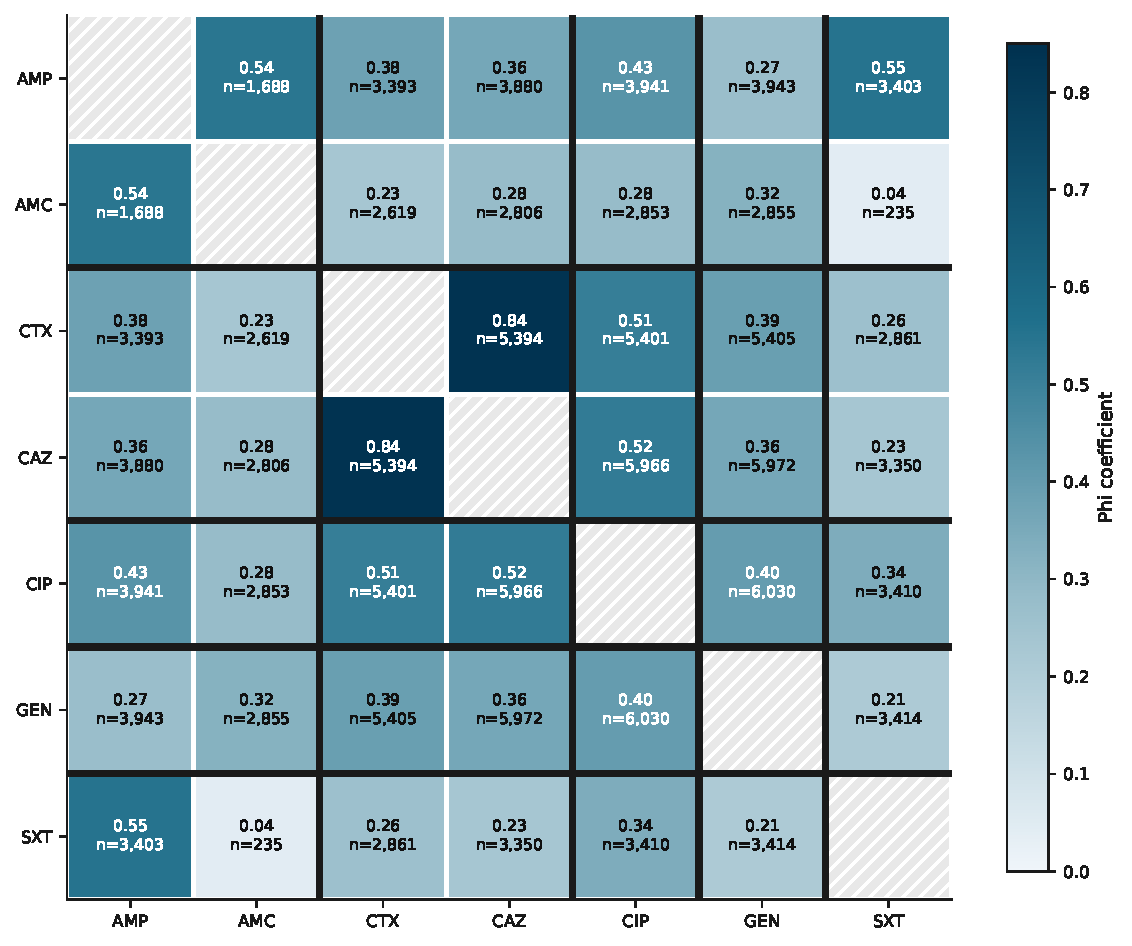
\includegraphics[width=0.62\textwidth]{fig_coresistance.pdf}
\caption{Pairwise co-resistance ($\phi$) between antibiotics, each cell computed on
the strains labelled for both drugs ($n$ shown). Lines separate drug classes.}
\label{fig:coresistance}
\end{figure*}

This influences the design that ensues. The cephalosporin connection would be
detected by a module that exchanged information solely inside classes (and not
between them), and it would fail to learn any cross-class link, which explains why
the class-specific heads below are initially succeeded by a refinement step that is
free to learn connections not present in the hierarchy.

This is implemented directly in the Cross-Antibiotic Context Module. Each gene's four
statistics are first transformed by a small multilayer perceptron (one per gene);
then, for global pooling across genes, gated attention is used to compute
$z_C \in \mathbb{R}^{64}$. This common representation is then decoupled into one
distinct projection for each drug class; the penicillins (AMP, AMC), the
cephalosporins (CTX, CAZ), the fluoroquinolone (CIP), the aminoglycoside (GEN), and
the folate-pathway inhibitor (SXT). All of the data prior to this split is learned
jointly from all seven drugs; all of the data after this is specific to one class,
\begin{equation}
t = \mathrm{GELU}(W_t z_C + b_t), \qquad
u_g = \mathrm{GELU}(W_g t + b_g),
\label{eq:expertC_trunk}
\end{equation}
where $t \in \mathbb{R}^{32}$ is the shared trunk output and
$u_g \in \mathbb{R}^{16}$ is the projection for drug class $g$. Now each antibiotic
reads its initial score, according to the projection of its own class only,
\begin{equation}
\ell^{\mathrm{init}}_{C,a} = w_a^\top u_{g(a)} + b_a,
\label{eq:expertC_ablogit}
\end{equation}
where $g(a)$ is the drug class antibiotic $a$ belongs to. Lastly, a co-resistance
refinement step allows the prediction for one antibiotic to modulate the prediction
for a related one,
\begin{equation}
r = \mathrm{MLP}\!\left(\left[z_C \, ; \, \ell^{\mathrm{init}}_{C}\right]\right),
\qquad
\ell_C = \ell^{\mathrm{init}}_{C} + \alpha\, r,
\label{eq:expertC_cores}
\end{equation}
with $\alpha$ a learned scalar starting with a value of 0.1. This step is initialised
to close to zero, such that the model initially ignores it, and only considers it
when the data supports the step which ensures that a spurious relationship between
two drugs is not baked in at the beginning.

It is easier to train seven separate models and this is how we started. The issue is
the lack of balance in drugs. The number of resistant strains of gentamicin is low
compared to ampicillin and therefore there is nothing much to learn by a
gentamicin-only model. There is a common base shared across all antibiotics. This
base learns from the labels of every drug, not just one. This is exactly what
multi-task learning is designed to do. Nonetheless, if the common base acquires a
misleading pattern, it influences all drugs. To limit this problem, there is a branch
for each drug. Some of those mistakes can still be corrected by these branches.

\subsection{Mixture-of-Experts Gating and Representation Fusion}
\label{subsec:moegate}

When each of three lenses has made an opinion about each of the seven antibiotics,
their opinions will not necessarily be consistent, and here the question is to what
to do with them. The easiest would be to average the three. We discarded that, since
averaging supposes that all the three lenses will be equally useful, and they are
not. When the resistance of a drug is due to an acquired plasmid gene, the Gene
Feature Attention Module should prevail and the Motif Pattern Encoder can do
practically nothing with it. In the case of a drug whose resistance is due to a point
mutation in a target enzyme, the opposite holds true. A decision based on the average
would drown out the voice of a stronger lens with two weaker ones.

The mixture-of-experts gate \cite{jacobs1991moe, shazeer2017moe} addresses this by
learning weights, rather than fixing them, and by learning them individually, one
strain at a time, and each antibiotic at a time. The three representations are
combined into a single vector $z = [z_A; z_B; z_C] \in \mathbb{R}^{192}$ and fed
through a small network and softmax to obtain
\begin{equation}
g = \mathrm{softmax}\big(\mathrm{MLP}([z_A; z_B; z_C])\big), \quad g \in \mathbb{R}^{B \times 7 \times 3},
\label{eq:moe_gate}
\end{equation}
so that for each antibiotic, the three weights are non-negative and sum to one. The
fused score of antibiotic $a$ is then the gate-weighted sum of the lens scores,
\begin{equation}
\ell^{\mathrm{fin}}_{a} = \sum_{e=1}^{3} g_{a,e}\,\ell_{e,a},
\qquad
p^{\mathrm{neu}}_{a} = \sigma\!\left(\ell^{\mathrm{fin}}_{a}\right).
\label{eq:fusion}
\end{equation}

One common failure mode of a gate of this type is often referred to in the literature
on mixture-of-experts as expert collapse, and is known here as gate collapse. It is
often the case that in the early stages of training, one of the lenses is a bit
better than the rest, by chance. This slight edge is noticed by the gate and makes it
transfer more weight onto that lens. The larger the gradient, the more weight. This
means that the lens will learn quicker and even more from the gate. After a few
epochs the other two lenses have ceased to be trained at all and the model silently
transforms into a single-lens network. To avoid this we count the spread out of the
gate with each antibiotic $a$ by its Shannon entropy,
\begin{equation}
H(g_a) = -\sum_{e=1}^{3} g_{a,e} \log g_{a,e},
\label{eq:gate_entropy}
\end{equation}
which is largest when the three weights $g_{a,e}$ are equal and smallest when the
gate has collapsed onto a single lens. Then we introduce an entropy term into the
loss, $-\lambda_{\mathrm{ent}}$ times the mean of $H(g_a)$ over the seven antibiotics,
\begin{equation}
\mathcal{L}_{\mathrm{ent}}
  = -\frac{\lambda_{\mathrm{ent}}}{7} \sum_{a=1}^{7} H(g_a)
  = \frac{\lambda_{\mathrm{ent}}}{7} \sum_{a=1}^{7} \sum_{e=1}^{3}
    g_{a,e} \log g_{a,e},
\label{eq:entropy_reg}
\end{equation}
that is minimized with a gate that spreads its weight and maximized with a gate that
concentrates its weight on one lens. With a small weight $\lambda_{\mathrm{ent}}$ this
pushes the gate to keep all three lenses active whilst leaving it free to favour one
where the evidence actually supports it. The symbol is written
$\lambda_{\mathrm{ent}}$, and not $\beta$, to keep it distinct from the $\beta$ of the
$F_\beta$ score in \eqref{eq:fbeta}. We track the average weight assigned to each lens
during training, and automatically increase the entropy weight when any lens's weight
goes below a threshold.

\subsection{Stacking Meta-Learner}
\label{subsec:metalearner}

The decision is eventually made by a logistic-regression meta-learner which combines
the neural probability with the five classical out of fold probabilities. This is
stacked generalisation in the sense of Wolpert \cite{wolpert1992stacked}, where the
predictions of multiple base learners are used as features for a second-level model.
Unlike simple averaging, the weighting is not fixed in advance; the six probabilities
are treated as inputs to a tiny model that learns from the data how much to trust
each of them. That is the difference between consulting six specialists and taking
the mean of their replies, and consulting six specialists whose respective track
records have been studied with a view to determining which of them is apt to be right
in which class of case.

The meta-learner constructs the feature vector $\phi_a$ of each antibiotic $a$,
\begin{equation}
\phi_a = \left[\,p^{\mathrm{neu}}_a,\; p^{(1)}_a,\; p^{(2)}_a,\; p^{(3)}_a,\; p^{(4)}_a,\; p^{(5)}_a\,\right],
\label{eq:meta_features}
\end{equation}
where $p^{(m)}_a$ are the probabilities of the five base learners, and calculates
\begin{equation}
\eta_a = w_a^\top \phi_a + b_a,
\qquad
\hat{p}_a = \sigma(\eta_a),
\label{eq:meta_logit}
\end{equation}
for each antibiotic, using an L2-penalised logistic regression with $C = 1.0$. It is
a conscious decision to train one meta-learner per antibiotic: the drugs are supposed
to rely on different models, and having a common meta-learner would push all seven to
make one trade-off. The final call is obtained by thresholding the probability,
\begin{equation}
\hat{y}_a = \mathbf{1}\!\left[\hat{p}_a > 0.5\right],
\label{eq:decision}
\end{equation}
with a fixed decision threshold of 0.5. We predict all seven antibiotics jointly, so
one forward pass through the model gives a full multi-label resistance profile.

We also tested a neural meta-learner. It is a more complex combination of the six
base predictions. The first step uses a small feed-forward layer to generate one
token per antibiotic. Subsequently, a four-head self-attention layer allows the seven
tokens to exchange information. Then, the final score of each drug is provided by a
separate decoding head. This was aimed at capturing co-resistance profiles, including
the cefotaxime-ceftazidime relationship. This drug-to-drug relationship cannot be
learnt by a separate linear model. The neural model, however, did not fare well. It
scored 0.825 against the simple meta-learner's 0.849. It was not the number of input
features that was the problem. The neural embedding is folded into the meta-feature
vector, bringing it to 170 dimensions. Nevertheless, there are only about 5{,}000
strains behind those numbers. The model is further complicated by the attention layer
and seven decoding heads. Consequently, it can easily fit noise in such a small
dataset. We can directly read the weights of the linear meta-learner, letting us see
more explicitly than a deeper meta-learner might allow how the final decision broke
down in terms of how much to trust the neural arm and how much to trust each
classical model for every antibiotic.

% ==== CUT FOR THE 30-PAGE LIMIT ====================================
% This subsection and its full-page table only recapped design decisions
% already argued in the text above, so nothing is lost. To restore it,
% delete the \iffalse below and the matching \fi after \end{table*}.
\iffalse
\subsection{Summary of Design Decisions}

Table~\ref{tab:designchoices} wraps up the primary design decisions defined in this
section along with the alternative that was considered and cause of the selection. In
cases wherein a decision was determined by measurement, not by argument, the numbers
in support of the decision are given in Section~\ref{sec:results}.

\begin{table*}[!tb]
\caption{Summary of the main design decisions and the alternatives considered.}
\label{tab:designchoices}
\centering
\small
\setlength{\tabcolsep}{5pt}
\renewcommand{\arraystretch}{1.05}
\begin{tabular}{|>{\raggedright\arraybackslash}p{3.2cm}|>{\raggedright\arraybackslash}p{3.4cm}|>{\raggedright\arraybackslash}p{9.6cm}|}
\hline
\rowcolor{headgrey}
\textbf{Decision} & \textbf{Alternative considered} & \textbf{Reason for the choice} \\ \hline
Hybrid neural and classical design & A single end-to-end neural network & With 6{,}962 samples against hundreds of thousands of features, a large network memorises rather than generalises. Gradient boosting is far more stable in this setting, and the neural arm supplies the interactions boosting cannot express. \\ \hline
Three genomic views & One combined feature matrix & Mutation based and gene presence based resistance are different mechanisms, and a single representation captures one at the cost of the other. \\ \hline
Convolution inside gene blocks & Convolution across the whole pan-genome & A shuffle test showed that variant ordering across the pan-genome carries no information, so convolution is only meaningful within a gene, where sequence order is real. \\ \hline
Attention over the gene profile & A dense layer over 32{,}441 genes & A dense layer would need tens of thousands of weights and would overfit immediately. Attention keeps the parameter count fixed and produces readable weights. \\ \hline
Shared trunk across antibiotics & Seven independent models & Groups of antibiotics within a class may have similar resistance mechanisms, so using one shared network allows drugs with more data to help drugs with less data. \\ \hline
Learned gate & Fixed average of the lenses & Different antibiotics rely on different lenses, and a fixed average would dilute the strongest opinion with two weaker ones. \\ \hline
Entropy regularisation on the gate & No regularisation & Without it the gate collapses onto one lens early in training and the other two stop learning. \\ \hline
Five classical base learners & One strong classical model & Ensembles gain from disagreement. The five were chosen to span linear and non-linear, high and low variance, and fine and coarse feature views. \\ \hline
Out-of-fold predictions & Predictions on the training data & Training-set predictions look better than they are, which would make the meta-learner trust the wrong models. \\ \hline
Logistic regression meta-learner & A deeper neural meta-learner & The signal available at this layer is six base probabilities per antibiotic; the deeper version widens that to a 170-dimensional vector but has only about 5{,}000 training rows behind it, and its weights would not be readable. It also scored lower. \\ \hline
Gene level features & Principal component features & Principal components mix genes together and cannot be named, which removes any possibility of interpretation, and they scored lower. \\ \hline
\end{tabular}
\renewcommand{\arraystretch}{1.0}
\end{table*}
\fi
% ==== END OF CUT ===================================================

\subsection{Implementation Details}
\label{subsec:common_framework}

All of the settings below are global across the model. Most follow traditional
practice and are therefore included for completeness; a few are less obvious and are
explained, where necessary.

\subsubsection{Binary Classification Setup}
In the case of each antibiotic, the model aims to predict either resistance (labelled
1) or susceptibility (labelled 0). The inputs are the three genomic views discussed
in the top-level overview and each raw score is transformed into a probability using
the logistic sigmoid from \eqref{eq:sigmoid}. All seven antibiotics are
predicted in the same forward pass, making it a multi-label problem instead of a
multi-class problem: a strain may be resistant to multiple drugs simultaneously and
the predictions do not have to compete with each other.

\subsubsection{Handling Class Imbalance}
Susceptible strains by far outnumber resistant ones for various drugs, which poses a
very real trap: a model predicting susceptible in all cases scores highly on accuracy
and is useless, but which is approximated well by a model that predicts the majority
class as the easiest way to minimize the loss. To avoid this, the resistant and
susceptible samples are reweighted in inverse proportion to their frequency of
occurrence, such that a mistake in getting a rare resistant strain is much costlier.
In the classical tree-based learners it can be accomplished by the
\texttt{scale\_pos\_weight} parameter,
\begin{equation}
\text{\texttt{scale\_pos\_weight}} = \frac{N_{\text{neg}}}{N_{\text{pos}}},
\label{eq:scale_pos_weight}
\end{equation}
where $N_{\text{neg}}$ and $N_{\text{pos}}$ are the numbers of susceptible and
resistant samples. In Logistic Regression and Random Forest, this is accomplished by
using balanced class weights, and in the neural lenses, by using positive class
weighting in the loss. For this reason, we use precision-recall AUC and not accuracy
during the evaluation as accuracy would conceal precisely the failure we want to
avoid.

\subsubsection{Threshold Selection}
\label{subsec:threshold_selection}
To arrive at the final decision, we use a constant probability threshold of 0.5 for
each of the antibiotics, as in \eqref{eq:decision}. This is the indifferent
option. It places the same emphasis on the two kinds of errors. But in clinical
practice this is not the case. The issue of predicting a resistant strain as being
susceptible can result in administering a drug that is not effective. The reverse
error is only going to result in picking another drug. A recall-oriented adjustment
was made according to the $F_{\beta}$ score,
\begin{equation}
F_{\beta} = \frac{(1 + \beta^2)\cdot\text{Precision}\times\text{Recall}}{\beta^2\cdot\text{Precision} + \text{Recall}},
\label{eq:fbeta}
\end{equation}
with $\beta = 2$ to give four times as much weight to recall as to precision, would
lower the threshold and capture more resistant strains while increasing the number of
false alarms. To avoid tuning the numbers in our favour, all headline results in this
research have been reported at the neutral threshold of 0.5 and then per-antibiotic
threshold tuning has been directly tested in Section~\ref{sec:results}, fitting the
threshold on validation and applying it to test.

\subsubsection{Optimization and Training Schedule}
The training of the neural lenses, the gate and the fusion step is done in a
simultaneous way, so that each lens learns to be useful in conjunction with the
others and not optimised alone. The objective consists of three terms: a binary
cross-entropy loss over the fused scores, the entropy regulariser in
\eqref{eq:entropy_reg}, and an auxiliary loss on each lens. This extra loss
term is important. In its absence, a lens which is momentarily disregarded by the
gate achieves extremely limited gradient. This leads to its cessation of improvement.
This problem is avoided by the auxiliary loss. It aids all lenses in continuing to
learn, even when they are not being selected by the gate. Optimization employs the
AdamW optimiser that keeps the weight decay and gradient update decoupled, and the
learning rate of $10^{-3}$, annealed on a cosine schedule over the epoch budget,
weight decay of $10^{-4}$, batch size of 16, gradient clipping of norm 1.0, and
mixed-precision training with the single exception described in
Section~\ref{subsec:lensB}, where the attention sum over 32{,}441 genes is kept at
single precision, with up to 50 epochs and early stopping after 8 consecutive
no-improvement epochs of validation mean precision-recall AUC. The inclusion of
gradient clipping is because, when attention is placed over 32{,}441 genes, the
gradients can sometimes be quite large, causing the training to become unstable. The
five classical base learners are trained individually via 5-fold cross validation,
with out-of-fold predictions, which are then used to fit the logistic-regression
meta-learner, along with the neural probabilities. The most important hyperparameters
are summarised in Table~\ref{tab:hyperparameters}.

\begin{table}[!tb]
\caption{Hyperparameter configuration for the classical base learners and the neural
model.}
\label{tab:hyperparameters}
\centering
\small
\setlength{\tabcolsep}{4pt}
\renewcommand{\arraystretch}{1.05}
\begin{tabular}{|>{\raggedright\arraybackslash}p{1.9cm}|>{\raggedright\arraybackslash}p{5.7cm}|}
\hline
\rowcolor{headgrey}
\textbf{Component} & \textbf{Key hyperparameters} \\ \hline
XGBoost (gene) & n\_estimators=1500; max\_depth=5; min\_child\_weight=5; learning\_rate=0.05; subsample=0.8; colsample\_bytree=0.7; reg\_alpha=0.1; reg\_lambda=1.0; gamma=0.1; tree\_method='hist'; early\_stopping\_rounds=150 \\ \hline
XGBoost (raw) & $\chi^2$-prefilter (top 50{,}000 SNPs); n\_estimators=1500; max\_depth=5; learning\_rate=0.05; subsample=0.8; colsample\_bynode=0.5; reg\_alpha=0.1; reg\_lambda=1.0; early\_stopping\_rounds=150 \\ \hline
LightGBM & n\_estimators=1500; num\_leaves=63; max\_depth=6; min\_child\_samples=20; learning\_rate=0.05 \\ \hline
Random forest & n\_estimators=200; max\_depth=12; min\_samples\_leaf=10 \\ \hline
Neural lenses and gate & AdamW; learning\_rate=$10^{-3}$ with cosine annealing; weight\_decay=$10^{-4}$; batch\_size=16; up to 50 epochs; early stopping patience 8; gradient clipping at norm 1.0; entropy weight $\lambda_{\mathrm{ent}}=0.01$ \\ \hline
Meta-learner & Logistic regression ($L_2$, $C=1.0$), one per antibiotic, fitted on 5-fold out-of-fold inputs \\ \hline
\end{tabular}
\renewcommand{\arraystretch}{1.0}
\end{table}

% =====================================================================
\section{Results}
\label{sec:results}
% =====================================================================

This section outlines what our models produced and what those numbers mean. First
we describe the measures that we used in evaluating performance and the results of
the proposed model, and then decompose the model, layer upon layer, to see where its
performance actually comes from. The remainder turns to the evidence that matters
most for this research's central claim: how the model behaves under a genuine
lineage holdout, on a separate collection, and when the genes it claims to rely on
are put to the test.

\subsection{Performance Evaluation}
\label{sec:perfeval}

The smaller group are the resistant strains, and even for a single antibiotic only
about one in five strains is resistant, so plain accuracy would not reveal the
problem: a model that declared every strain susceptible would still seem accurate,
but would be useless in a clinic. The primary metric that we are interested in is
the area under the precision--recall curve (PR-AUC), which captures the performance
of a model in terms of precision-recall at all threshold levels and does not
encourage a model to make majority class predictions. It is defined as
\begin{equation}
\text{PR-AUC} = \sum_{n} \left( R_n - R_{n-1} \right) P_n
\end{equation}
where $P_n$ and $R_n$ are the precision and recall at the $n$-th threshold.

We also report a few other measures, since there is no single number which tells the
entire story. Matthews Correlation Coefficient (MCC) employs all four cells of the
confusion matrix simultaneously, and remains truthful in case of imbalanced classes:
\begin{equation}
\resizebox{0.93\columnwidth}{!}{$\displaystyle
\text{MCC} = \frac{TP \times TN - FP \times FN}
{\sqrt{(TP+FP)(TP+FN)(TN+FP)(TN+FN)}}$}
\end{equation}
MCC can be between $-1$ and $+1$ (where $0$ indicates model guessing), and all
values are calculated per antibiotic using a one-versus-rest approach. We also report
the two members of the $F_\beta$ family of \eqref{eq:fbeta} that this work uses,
obtained by setting $\beta = 1$ and $\beta = 2$ in that expression: $F_1$ is the
harmonic mean of precision and recall, and $F_2$ weights recall four times higher,
since failing to identify a drug-resistant strain is worse than falsely labelling a
susceptible strain resistant.

We show accuracy for thoroughness, but we do not use it. Measures of machine
learning are inadequate by themselves to tell a clinician whether a tool is safe, and
so we also report the microbiology vocabulary. A \emph{very major error} (VME) is a
resistant strain called susceptible, which is the dangerous case; a \emph{major
error} (ME) is the reverse, which costs a drug option but does not put the patient
directly at risk; and \emph{categorical agreement} (CA) is the proportion of strains
on which our call matched the laboratory result. All these evaluations determine
three things: the degree to which the model ranks strains well (PR-AUC), the degree
to which it makes balanced decisions at some threshold (MCC, F1, F2), and whether its
errors would be tolerated in a hospital (VME, ME, CA).

\begin{table}[!tb]
\caption{TriLens-MoE-Stack on the random split, per antibiotic.}
\label{tab:main}
\centering
\small
\setlength{\tabcolsep}{4pt}
\renewcommand{\arraystretch}{1.05}
\begin{tabular}{|l|r|r|r|r|r|}
\hline
\rowcolor{headgrey}
\textbf{Drug} & \textbf{PR-AUC} & \textbf{MCC} & \textbf{F1} & \textbf{F2} & \textbf{Acc.} \\ \hline
CIP & \textbf{0.9773} & 0.9088 & 0.9282 & 0.9197 & 0.9692 \\ \hline
AMP & 0.9440 & 0.7866 & 0.8932 & 0.8917 & 0.8933 \\ \hline
CTX & 0.9019 & 0.7904 & 0.8173 & 0.8126 & 0.9530 \\ \hline
SXT & 0.8352 & 0.6954 & 0.7875 & 0.7730 & 0.8707 \\ \hline
CAZ & 0.8299 & 0.6928 & 0.7290 & 0.7169 & 0.9356 \\ \hline
AMC & 0.7482 & 0.5237 & 0.6563 & 0.6250 & 0.8035 \\ \hline
GEN & \textbf{0.7037} & 0.6095 & 0.6386 & 0.5915 & 0.9341 \\ \hline
\rowcolor{oursblue}
\textbf{Average} & \textbf{0.8486} & \textbf{0.7153} & \textbf{0.7786} & \textbf{0.7615} & \textbf{0.9085} \\ \hline
\end{tabular}
\renewcommand{\arraystretch}{1.0}
\vspace{0.4em}

\noindent\footnotesize\textit{Note:} Ciprofloxacin has the highest PR-AUC (0.9773) and
gentamicin the lowest (0.7037), the spread the text below discusses; the last row averages
across all seven antibiotics. Bold marks the extreme values in a column, best and worst alike.
\end{table}

The average PR-AUC is 0.849, yet the average conceals a broad distribution, and the
interesting part is the spread. The clearest case is ciprofloxacin, at 0.9773 with
MCC 0.9088, which is close to a practical ceiling for this kind of data, followed by
ampicillin at 0.9440. On the other hand, gentamicin comes in at 0.7037 and
amoxicillin-clavulanate at 0.7482, meaning the spread of best to worst is nearly 0.27
for models trained of exactly the same genomes with the exact same architecture.

The accuracy column is different from the others. Gentamicin has the lowest PR-AUC
value, but high accuracy value of 0.9341 as the proportion of strains resistant to
gentamicin is small, so a model can achieve a high accuracy, but fail to detect many
resistant strains. This is the same trap as above, and the reason accuracy is not our
primary measure. As far as a hospital is concerned, it is the type of error that the
model produces, of which the results are documented in Table~\ref{tab:clinical}.

\begin{table}[!tb]
\caption{Clinical error rates at a threshold of 0.5, ordered by very major error
rate.}
\label{tab:clinical}
\centering
\small
\setlength{\tabcolsep}{4pt}
\renewcommand{\arraystretch}{1.05}
\begin{tabular}{|l|r|r|r|l|}
\hline
\rowcolor{headgrey}
\textbf{Drug} & \textbf{VME} & \textbf{ME} & \textbf{CA} & \textbf{Meets CLSI} \\ \hline
CIP & \textbf{0.086} & 0.015 & 0.969 & No (ME only) \\ \hline
AMP & 0.109 & 0.104 & 0.893 & No \\ \hline
CTX & 0.190 & 0.026 & 0.953 & No (ME only) \\ \hline
SXT & 0.236 & 0.080 & 0.871 & No \\ \hline
CAZ & 0.291 & 0.033 & 0.936 & No \\ \hline
AMC & 0.394 & 0.108 & 0.804 & No \\ \hline
GEN & \textbf{0.436} & 0.023 & 0.934 & No (ME only) \\ \hline
\end{tabular}
\renewcommand{\arraystretch}{1.0}
\vspace{0.4em}

\noindent\footnotesize\textit{Note:} Ciprofloxacin has the lowest very major error (VME) rate at
0.086 and gentamicin the highest at 0.436. No antibiotic meets both CLSI limits at once;
``No (ME only)'' means only the major-error limit is met.
\end{table}

Ciprofloxacin reappears as the strongest, having a VME of 0.086, and a categorical
agreement of 0.969. Gentamicin is weakest with 0.436 (almost half of all resistant
strains would be reported sensitive) and amoxicillin-clavulanate is almost as poor
(0.394). The ordering is important, as an almost identical ordering is rediscovered
under the lineage holdout in Section~\ref{subsec:prevmatch} in an entirely different
way.

The categorical agreement column is the same as the accuracy column of
Table~\ref{tab:main}, and this is not by chance. During data preparation the
intermediate results were grouped with the resistant results, so the intermediate
category no longer exists in this dataset. Categorical agreement therefore reduces to
binary accuracy here. Gentamicin illustrates this point clearly, with a categorical
agreement of 0.934 versus a VME of 0.436. On the same strains, the same model is seen
to be strong by one measure and unusable by the other.

The CLSI limits require both the VME and ME rates to stay under three percent
\cite{clsi_m52}. Three antibiotics satisfy the major error limit, which are
ciprofloxacin at 0.015, gentamicin at 0.023 and cefotaxime at 0.026 but none satisfy
the very major error limit, therefore, the model is not yet prepared to be used as a
diagnostic test.

Two qualifications apply to that comparison, and the second is the more serious of
them. The first is that the limits are written for the verification of a commercial
susceptibility testing system against a challenge panel that is deliberately enriched
for resistant and near-breakpoint isolates, whereas we apply them to a retrospective
genomic model on a convenience collection; a passing score here would not constitute
regulatory evidence, and we use the limits only because they are the closest published
statement of what error rate a laboratory will tolerate. The second is that we
collapsed the intermediate category into resistant, so our three rates are computed on
a two-category comparison, while the standard defines them on the three-category
susceptible, intermediate and resistant comparison and excludes certain
intermediate-involving discrepancies from the counts altogether. Collapsing in this
direction moves genuinely intermediate strains into the resistant class, which can only
raise our apparent very major error rate relative to the standard definition and
leaves the major error rate essentially unaffected. The direction of the bias is
therefore against us and the conclusion that no antibiotic clears the very major error
limit is safe, but the individual rates are not the same quantity the standard
tabulates and should not be quoted as though they were.

The obvious response is that the fixed 0.5 threshold was never tuned to clinical
cost, and that the numbers above could be an artefact of positioning the cut. To do
this, we trained a threshold for each antibiotic on the validation set, constraining
the $F_2$ objective of \eqref{eq:fbeta} and capping the major error rate,
and assessed each on the test set. While the tuning for $F_2$ moves the mean very
major error rate only from 0.249 to 0.210, still far above the limit of 0.03, and
forcing the major error rate to remain inside the limit pushes the mean very major
error rate to 0.437, neither rescues the model. In fact, none of the antibiotics was
able to achieve both thresholds at any threshold value that we tested, because
shifting the cut trades one kind of error against the other instead of cutting down
on both. It is not the position of the cut that drives the clinical shortfall,
however, but the model's ability to separate the two classes. As such, future work
should not focus on calibration, but on the feature representation.

\subsection{Statistical Analysis}
\label{sec:statanalysis}

In our test set there are 1{,}045 strains and in some antibiotics there are only a
few hundred of known label, so one or two points difference can be simply accidental.
We resampled the test set (1{,}000 bootstrap resamples with replacement) to
recalculate PR-AUC, and used the 2.5th and 97.5th percentiles as a 95\% confidence
interval. The result is shown in Table~\ref{tab:ci} and plotted in
Fig.~\ref{fig:ci_forest} as the intervals against the no-skill baseline of the
individual drugs, i.e., the range within which the raw scores are most misleading: a
PR-AUC has to be read against the prevalence of the drug it represents, not against
the other drugs in the column. The PR-AUC of ampicillin, 0.944, sits above a no-skill
baseline of roughly one resistant strain in two. The score of gentamicin, 0.7037,
appears smaller in absolute terms, but its no-skill baseline is only about one
resistant strain in ten. Gentamicin's raw score is lower, yet it is the greater gain
over chance.

\begin{table}[!tb]
\caption{Bootstrap confidence intervals for the proposed model on the random-split
test set, from 1{,}000 resamples.}
\label{tab:ci}
\centering
\small
\setlength{\tabcolsep}{4pt}
\renewcommand{\arraystretch}{1.05}
\begin{tabular}{|l|r|l|}
\hline
\rowcolor{headgrey}
\textbf{Drug} & \textbf{PR-AUC} & \textbf{95\% confidence interval} \\ \hline
AMP & 0.9440 & [0.919, 0.965] \\ \hline
CIP & 0.9773 & \textbf{[0.961, 0.990]} \\ \hline
AMC & 0.7482 & [0.680, 0.809] \\ \hline
SXT & 0.8352 & [0.773, 0.891] \\ \hline
GEN & 0.7037 & \textbf{[0.612, 0.786]} \\ \hline
CTX & 0.9019 & [0.851, 0.943] \\ \hline
CAZ & 0.8299 & [0.762, 0.882] \\ \hline
\rowcolor{oursblue}
\textbf{Average} & \textbf{0.8486} & \textit{not defined} \\ \hline
\end{tabular}
\renewcommand{\arraystretch}{1.0}
\vspace{0.4em}

\noindent\footnotesize\textit{Note:} Ciprofloxacin's interval, [0.961, 0.990], is the tightest in
the table, backed by the most labelled data; gentamicin's, [0.612, 0.786], is the widest,
backed by the least. No interval is given for the average, because the seven per-drug
resamples are drawn from overlapping strain sets and their intervals are therefore not
independent; the average is reported as a point summary only. Bold marks the extreme
values in a column, best and worst alike.
\end{table}

\begin{figure}[!tb]
\centering
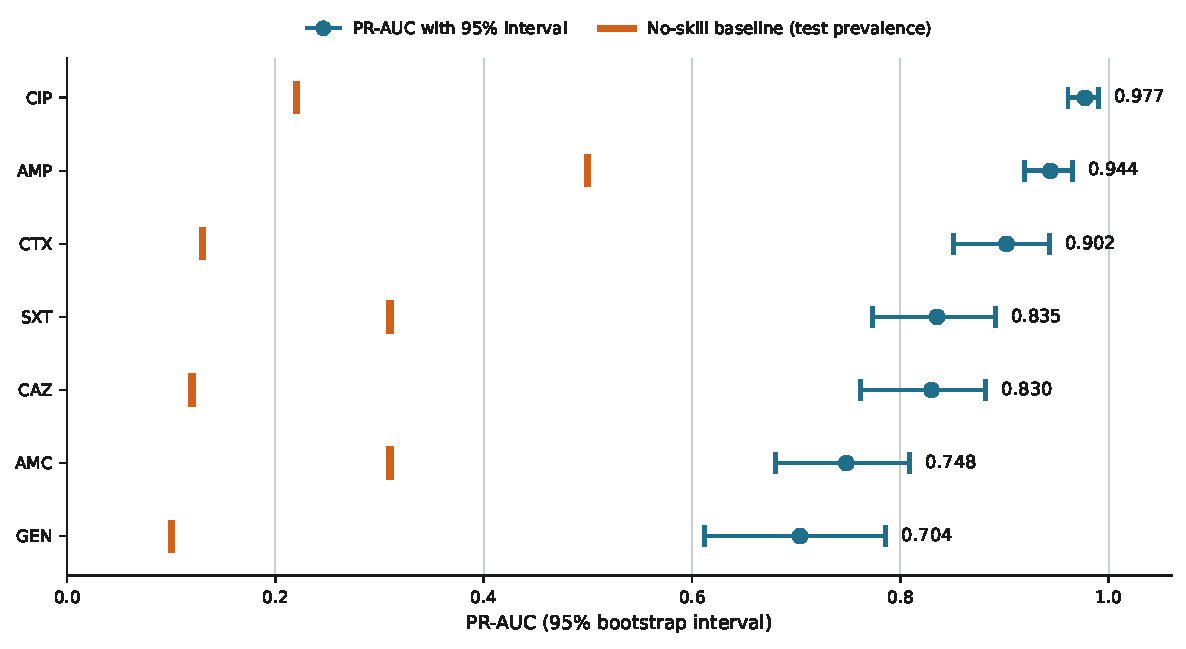
\includegraphics[width=\columnwidth]{fig_ci_forest.pdf}
\caption{PR-AUC with 95\% bootstrap intervals, against each antibiotic's no-skill
baseline (test-set prevalence).}
\label{fig:ci_forest}
\end{figure}

Gentamicin ranges 0.612 to 0.786, a range of nearly 0.18, and this is simply the
result of few resistant strains, but ciprofloxacin, which has more labelled strains
and a stronger signal, has a much smaller range. Any difference between two models on
this test set must therefore exceed this interval width before it can be termed
significant. None of the differences reported in this section between closely related
methods clears that bar.

One limit of these intervals should be stated plainly, because it governs how every
architectural comparison in this section may be read. A bootstrap over the test set
quantifies the variability that comes from which strains happen to fall in the test
partition. It does not quantify the variability that comes from training itself. Every
model reported here was trained once, under the single fixed seed of
Section~\ref{subsec:splits}, so the effect of initialisation, of batch ordering and of
the stochastic elements of the classical learners is not represented in any interval we
report. Differences of the order of a few thousandths of PR-AUC, such as the $+0.009$
that separates the full model from the strongest single classical learner in
Section~\ref{subsec:layerabl} or the $+0.0024$ that strain conditioning buys on the random
split in Section~\ref{subsec:strainablation}, are therefore of a size that seed
variation alone could plausibly produce, and we do not claim them as real effects. We
treat as established only those differences that are large relative to the interval
widths above, namely the gap between the random split and the lineage holdout and the
gap between the two groups of antibiotics. The $+0.035$ that strain conditioning
delivers to the neural lenses alone under the holdout sits between the two cases: it is
an order of magnitude larger than the same term's effect on the random split, and it
moves three interpretability measures with it, which is more than a seed artefact would
be expected to do, but on its own it does not clear the interval widths either.
Repeating the full protocol over several seeds, and reporting a mean and standard
deviation for each cell, is the natural next step and is the first item of future work
in Section~\ref{sec:conclusion}.

A second robustness check belongs with these intervals. Some
bacterial collections have nearly identical strains. If one of the copies ends up
in training and the other ends up in the test set, the model may score well on this
task simply by recognizing something it has already seen, so we checked for this
reason. To assess this, we calculated the Hamming distance from each test strain to
its nearest training strain. The closest pair differed by only 0.26\% of their SNP
positions, and, out of 1{,}045 test strains, 47 were within 0.5\% of a training
strain, which are considered ``effectively duplicates.'' The 0.5\% cut is a working
threshold and not a standard one: on the 535{,}439-position matrix it corresponds to
roughly 2{,}700 differing positions, which is an order of magnitude below the typical
separation of two strains of the same sequence type in this collection, so pairs
inside it are far closer than clonality alone would explain. We report the sensitivity
of the result to that choice below rather than resting on the cut itself.

Then, we removed these 47 strains, and scored the model anew on the remainder.
PR-AUC decreased on average by 0.0041, with ceftazidime falling by the largest, of
0.0209, and amoxicillin-clavulanate increasing by 0.0075. It is very slight and not
directional, which informs us that near-duplicates will not be the primary factor
that supports our findings. Nonetheless, it remains a real effect and reporting the
deduplicated number provides a truthful lower bound.

\subsection{Component Ablation}
\label{subsec:layerabl}

Each neural lens reads a different part of the genome and a gate determines the
trustworthiness of each lens, with five classical learners combined by a stacking
layer. To determine whether each part is warranted, we removed each component in turn
and measured the impact on performance. We trained three variants using the same
data, seed and test set. \textbf{Stage 1} is the three lenses only; they average
their outputs with equal weighting and no gate is used. \textbf{Stage 2} is the three
lenses and the mixture-of-experts gate, such that the model learns the extent to
which to rely on individual lenses on individual samples and antibiotics; this is the
neural part of the model on its own. \textbf{Stage 3} is the complete model in which
the neural output is appended with the five classical base learners via the
meta-learner. Table~\ref{tab:ablation} shows the result.

\begin{table*}[!tb]
\caption{Component ablation on the random split, with the PR-AUC gain each added part
contributes over the stage before it.}
\label{tab:ablation}
\centering
\small
\setlength{\tabcolsep}{5pt}
\renewcommand{\arraystretch}{1.05}
\begin{tabular}{|l|r|r|r|r|r|r|r|r|r|}
\hline
\rowcolor{headgrey}
\textbf{Stage} & \textbf{AMP} & \textbf{CIP} & \textbf{AMC} & \textbf{SXT} & \textbf{GEN} & \textbf{CTX} & \textbf{CAZ} & \textbf{Avg} & \textbf{Gain} \\ \hline
Stage 1: lenses only    & 0.8920 & 0.9248 & 0.6249 & 0.7217 & 0.5168 & 0.8103 & 0.7267 & 0.7453 & N/A \\ \hline
Stage 2: + MoE gate     & 0.8970 & 0.9489 & 0.6347 & 0.7453 & 0.5835 & 0.8659 & 0.7893 & 0.7807 & $+0.0353$ \\ \hline
\rowcolor{oursblue}
Stage 3: + stacking     & 0.9440 & 0.9773 & 0.7482 & 0.8352 & 0.7037 & 0.9019 & 0.8299 & \textbf{0.8486} & \textbf{$+0.0679$} \\ \hline
\end{tabular}
\renewcommand{\arraystretch}{1.0}
\vspace{0.4em}

\noindent\footnotesize\textit{Note:} The full model reaches an average PR-AUC of 0.8486;
classical stacking adds $+0.0679$ over stage 2, about twice the gate's own $+0.0353$ contribution.
\end{table*}

There are two points that are established. First, there is no dead weight: for each
and every antibiotic, the performance improves when it goes from Stage 1 to Stage 2
and then to Stage 3. Second, the parts do not aid equally. Combining neural
predictions with classical learners achieves on average about 0.0679 more than the
neural design alone, while the gate achieves only 0.0353. The neural lenses are
useful, but not sufficient by themselves, and thus the final model is best referred
to as a hybrid rather than as a neural model.

The average weight assigned to each lens by the gate is shown in
Table~\ref{tab:gate}, and the weights by antibiotic in
Fig.~\ref{fig:gate_routing}.

\begin{table}[!tb]
\caption{Average gate weights on the test set. Each row sums to one.}
\label{tab:gate}
\centering
\small
\setlength{\tabcolsep}{4pt}
\renewcommand{\arraystretch}{1.05}
\begin{tabular}{|l|r|r|r|}
\hline
\rowcolor{headgrey}
\textbf{Drug} & \textbf{Lens A} & \textbf{Lens B} & \textbf{Lens C} \\ \hline
AMP & 0.070 & 0.852 & 0.078 \\ \hline
CIP & \textbf{0.035} & 0.590 & 0.374 \\ \hline
AMC & 0.095 & 0.742 & 0.163 \\ \hline
SXT & 0.052 & \textbf{0.900} & 0.047 \\ \hline
GEN & 0.098 & 0.731 & 0.171 \\ \hline
CTX & 0.064 & 0.815 & 0.121 \\ \hline
CAZ & 0.044 & 0.835 & 0.122 \\ \hline
\end{tabular}
\renewcommand{\arraystretch}{1.0}
\vspace{0.4em}

\noindent\footnotesize\textit{Note:} Ciprofloxacin's Lens A weight of 0.035 is the lowest in the
table despite being the drug that lens was built for, and trimethoprim-sulfamethoxazole's Lens B
weight of 0.900 is the highest, closest to gate collapse; both are discussed below.
\end{table}

\begin{figure}[!tb]
\centering
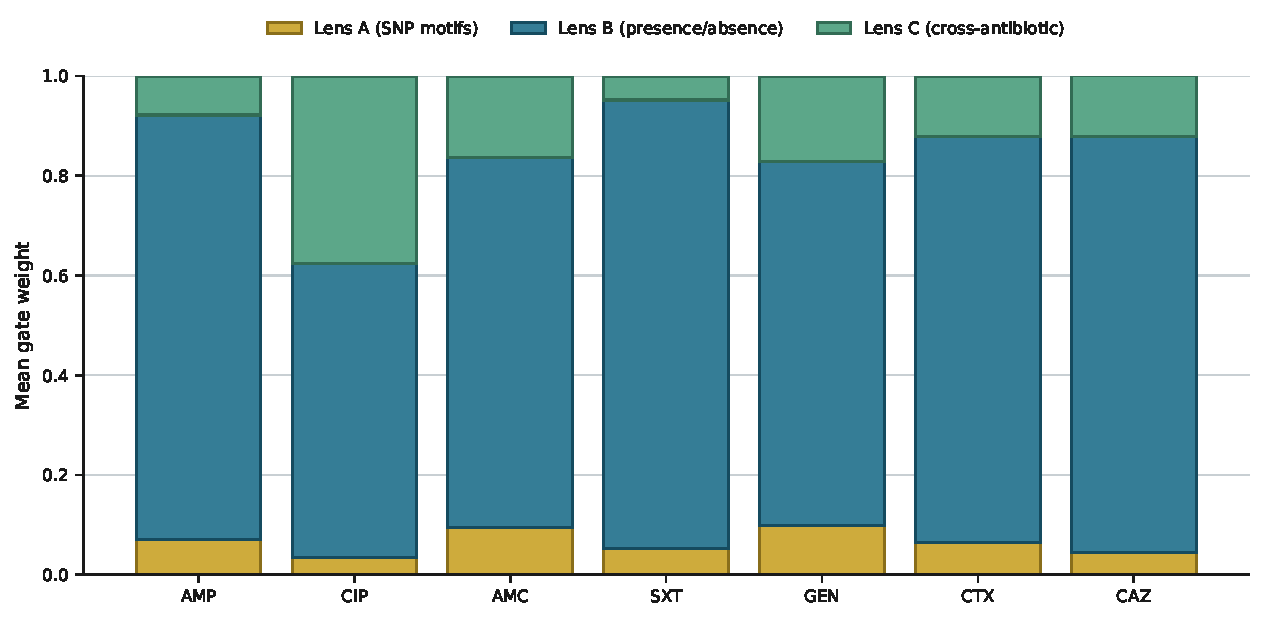
\includegraphics[width=\columnwidth]{fig_gate_weights.pdf}
\caption{Mean gate weight assigned to each lens, by antibiotic, on the test set. The
three weights sum to one for each antibiotic; these are the values of
Table~\ref{tab:gate} drawn as stacked bars.}
\label{fig:gate_routing}
\end{figure}

The trend is the same. Most of the weight of each antibiotic, 0.590 to 0.900, is in
Lens B, which reads which genes are present or absent, whereas Lens A, the
convolutional lens reading mutation patterns within genes, never goes above 0.098. At
least this is consistent with the biology as a large part of the resistance in
\textit{E. coli} is conferred by acquired genes.

Ciprofloxacin is where the table stops agreeing with the design. The rationale for
the gate in Section~\ref{subsec:moegate} is a prediction: a drug whose resistance is
based on an acquired gene should route to Lens B, whereas a drug whose resistance is
based on a point mutation in a target enzyme should route to Lens A. Ciprofloxacin is
the most obvious point-mutation drug that we have in our panel, and the one that our
SHAP analysis suggests is related to \textit{gyrA} and \textit{parC}; yet Lens A
receives 0.035 for this drug, the lowest value in the table. The prediction fails on
the one antibiotic where it was most testable. This is the highest value for Lens C,
but it is difficult to read from either direction. The lens shares drug-class head
evidence, but ciprofloxacin is the only fluoroquinolone in the panel and has no
same-class partner, and although its co-resistance refinement step may still link
ciprofloxacin to ceftazidime, which shares $\phi = 0.52$ in this collection
(Fig.~\ref{fig:coresistance}), that is co-occurrence rather than mechanism. On
neither reading can 0.374 be taken as the gate finding the mechanism.

The gate therefore tells us which lens the model relies on, which is worth knowing,
but its routing is not in the direction the design assumed. The same
conclusion is drawn in the attention audit in Section~\ref{subsec:markers}. A second
reading of the table points the same way. In the final weights,
trimethoprim-sulfamethoxazole reaches 0.900. Three more drugs sit above 0.81:
ampicillin at 0.852, ceftazidime at 0.835, and cefotaxime at 0.815. It seems that the
penalty would have slowed, but not stopped, collapse, and therefore, these weights
are possibly associated with optimisation-like dynamics as well as with biology.

Table~\ref{tab:baselines} distinguishes between two similar but different questions.
The first is the comparison of the proposed model with external models. There are
three external baselines: a null model using only the phylogroup label, TabNet and
the gradient-boosting model using principal component analysis (PCA) components
that this project began with. The
second question is what each component of the proposed system contributes to the
overall result. With this in mind, the five base learners are tested individually as
well. But these are not external baselines. The proposed system consists of multiple
learners, each feeding the meta-learner. Thus, comparing these learners with the full
system is not an external comparison, but rather an ablation. All models were
evaluated with the same data splits and the same five-fold protocol. The values
reported are the mean PR-AUC scores of the seven antibiotics.

\begin{table}[!tb]
\caption{Comparisons of the proposed model with external baselines and results of the
component models. The phylogroup-only and PCA baselines were not evaluated with the
lineage holdout.}
\label{tab:baselines}
\centering
\footnotesize
\setlength{\tabcolsep}{3pt}
\renewcommand{\arraystretch}{1.05}
\begin{tabular}{|l|r|r|}
\hline
\rowcolor{headgrey}
\textbf{Model} & \textbf{Random split} & \textbf{Lineage holdout} \\ \hline
\multicolumn{3}{|l|}{\textit{External baselines}} \\ \hline
Phylogroup label only & 0.2914 & not run \\ \hline
TabNet & 0.6951 & 0.3255 \\ \hline
XGBoost on 1{,}024 PCA components & 0.8033 & not run \\ \hline
\multicolumn{3}{|l|}{\textit{Components of the proposed system}} \\ \hline
Random Forest, gene features & 0.7809 & 0.4931 \\ \hline
Logistic Regression, gene features & 0.7923 & 0.4408 \\ \hline
LightGBM, gene features & 0.8338 & 0.5516 \\ \hline
XGBoost, gene features & 0.8375 & 0.5507 \\ \hline
XGBoost, $\chi^2$-filtered SNPs & 0.8400 & 0.6299 \\ \hline
\rowcolor{oursblue}
\textbf{TriLens-MoE-Stack} & \textbf{0.8486} & \textbf{0.6337} \\ \hline
\end{tabular}
\renewcommand{\arraystretch}{1.0}
\vspace{0.4em}

\noindent\footnotesize\textit{Note:} The last row is the proposed model, the one every other row
in the table is being measured against.
\end{table}

On the random split the model produces the highest score of all entries in the table.
If only the eight-way phylogroup label is used as a baseline, the PR-AUC reaches just
0.2914, against a mean resistance frequency across the seven drugs of 0.250, which is
effectively the floor for this task. Coarse lineage membership therefore buys about
0.04 over chance and no more. The specialized tabular deep-learning
baseline, TabNet, achieves only 0.6951, behind every single classical learner, and
falls to 0.3255 under the lineage holdout, where even the weakest classical learner
still reaches 0.4408: added depth does not help on this problem under either test.
The five classical learners themselves range from PR-AUC 0.7809 to 0.8400, with the
three gradient-boosting models on the higher end of that span. The highest entry in
the table, at 0.8486, is TriLens-MoE-Stack, which leads every external baseline on the
average and is ahead of its own strongest component on five of the seven antibiotics.

It is not just the direction of the result that matters, but also the size of the
improvement. The proposed model outperforms the PCA baseline by 0.0453, TabNet by
0.1535 and the null model by 0.5572. The PCA comparison is the most telling as it
demonstrates what this project contributed, since this project began with the PCA
model. For individual antibiotics, the proposed model has scores above the upper
limit of the baseline interval for ampicillin, ciprofloxacin and
trimethoprim-sulfamethoxazole. Its score is within the interval for the other four
antibiotics.

\subsection{Comparison with Published \textit{E. coli} Studies}
\label{subsec:sota}

Table~\ref{tab:sota} places this work beside the published \textit{E. coli} studies
of Table~\ref{tab:summary}, restricted to those working on a comparable collection
and task. The headline figures in the fourth column are not directly comparable
with one another, because the collections, the drug panels and the reported
measures all differ, and Section~\ref{subsec:prevmatch} shows that a score cannot
be read without the prevalence behind it. The column that carries the argument is
the fifth: of the five earlier studies, one withholds a lineage and reports the
result only as a supplementary analysis, one leaves an MLST-blocked split available
as an option it does not use for its headline number, and three do not test on an
unseen lineage at all. None corrects for the prevalence shift the holdout produces.

\begin{table*}[!tb]
\caption{This work against published \textit{E. coli} resistance-prediction studies
drawn from Table~\ref{tab:summary}. The reported-result column is quoted as each
study states it and the entries are not directly comparable, as the collections,
drug panels and measures differ; the final column records whether the study tests
on a lineage it never trained on.}
\label{tab:sota}
\centering
\footnotesize
\setlength{\tabcolsep}{3pt}
\renewcommand{\arraystretch}{1.05}
\begin{tabular}{|>{\raggedright\arraybackslash}p{2.7cm}|>{\raggedright\arraybackslash}p{3.2cm}|>{\raggedright\arraybackslash}p{3.8cm}|>{\raggedright\arraybackslash}p{2.9cm}|>{\raggedright\arraybackslash}p{3.4cm}|}
\hline
\rowcolor{headgrey}
\textbf{Study} & \textbf{Collection and drugs} & \textbf{Evaluation split} & \textbf{Reported result} & \textbf{Tested on an unseen lineage?} \\ \hline
Moradigaravand et al.\ (2018) \cite{moradigaravand2018} & 1,936 \textit{E. coli}, 11 compounds & Random, with an ST131 lineage holdout as a supplementary analysis & Gradient boosting best of the three learners & Yes, but only as a supplementary analysis; the ST131 holdout scores about 0.28 below a size-matched random control \\ \hline
Her and Wu (2018) \cite{her2018pangenome} & 59 \textit{E. coli}, 12 drugs & Leave-one-out cross-validation & Accessory genome carried most signal & No \\ \hline
Ren et al.\ (2022) \cite{Ren2022} & Giessen (987) and public (1,509) \textit{E. coli} & Stratified cross-validation with an independent external set & RF best, AUC around 0.96 & No \\ \hline
Orcales et al.\ (2024) \cite{Orcales2024} & 1,936 \textit{E. coli} & Cross-validation, with an MLST-blocked option & XGBoost most reliable & Available as an option, not used for the headline result \\ \hline
Siddiqui and Tarannum (2026)\textsuperscript{$\dagger$} \cite{siddiqui2025amrensemble} & Giessen (809) \textit{E. coli}, 4 antibiotics & Stratified 80/20 holdout & MCC 0.926 for CIP, macro F1 0.691 for GEN & No \\ \hline
\rowcolor{oursblue}
\textbf{This work} & \textbf{6,962 \textit{E. coli}, 7 antibiotics} & \textbf{Random, phylogroup-stratified and sequence-type lineage holdout} & \textbf{PR-AUC 0.849 on the random split} & \textbf{Yes, as the primary design: 0.634 as measured and 0.723 once the test set is resampled to the training prevalence} \\ \hline
\end{tabular}
\renewcommand{\arraystretch}{1.0}
\vspace{0.4em}

\noindent\footnotesize\textit{Note:} The last row is this work. Bold marks that row
and not a best result, because the fourth column is not a like-for-like comparison.
\textsuperscript{$\dagger$}Prior work of one of the present authors.
\end{table*}

\subsection{The Lineage Holdout}
\label{subsec:prevmatch}

The question posed in this subsection is more difficult: does the model continue to
work when it is presented with a strain it has never seen before? The
phylogroup-stratified split fails to do it: it rearranges the information within
eight large clusters, thus leaving a strain and a close one on different sides, and
its performance under it changes little, between 0.849 and 0.853. This is not a test
of unfamiliar strains, and therefore could not have indicated a drop in any way.

The holdout which answers it makes use of the type of sequence of each strain, a
common designation of bacterial genetics according to which strains are clustered by
lineage. We successfully called a type of sequence to 6,487 of the 6,962 strains, or
93.2\%, with a total of 458 types, including a couple of giant ones: sequence
type 73 alone has 884 strains, or nearly one in every eight of the samples. There
were two rules prior to peeking at any outcome. Any strain whose sequence type had no
reliable sequence type was put into training and here, any sequence type that
comprised over five percent of the data was also put into training, as a test set
constructed using mostly a single clone would not be testing generalisation. That
condition was fulfilled by four types, namely, ST73, ST131, ST95 and ST69. The other
454 sequences were assigned whole (not split), using a fixed random seed such that no
sequence type appears in more than one of the training, validation and test sets.

The outcome was just the opposite. Mean performance plummets to 0.634 when they are
split by the lineage holdout, a decrease of over a fifth, and that is what the
phylogeny split had been unable to discover since it did not wipe any lineage off
training. Table~\ref{tab:mlst_per_ab} positions the three splits next to each other.

\begin{table}[!tb]
\caption{Per-antibiotic PR-AUC under all three splits, with the drop measured from
the random split to the lineage holdout.}
\label{tab:mlst_per_ab}
\centering
\small
\setlength{\tabcolsep}{4pt}
\renewcommand{\arraystretch}{1.05}
\begin{tabular}{|l|r|r|r|r|}
\hline
\rowcolor{headgrey}
\textbf{Drug} & \textbf{Random} & \textbf{Phylogroup} & \textbf{Holdout} & \textbf{Drop} \\ \hline
AMP & 0.9440 & 0.9338 & 0.9043 & $\mathbf{-0.040}$ \\ \hline
SXT & 0.8352 & 0.8373 & 0.7872 & $-0.048$ \\ \hline
CIP & 0.9773 & 0.9617 & 0.9118 & $-0.066$ \\ \hline\hline
AMC & 0.7482 & 0.7963 & 0.4865 & $-0.262$ \\ \hline
CTX & 0.9019 & 0.8807 & 0.6073 & $-0.295$ \\ \hline
CAZ & 0.8299 & 0.8481 & 0.4930 & $-0.337$ \\ \hline
GEN & 0.7037 & 0.7136 & 0.2457 & $\mathbf{-0.458}$ \\ \hline
\rowcolor{oursblue}
\textbf{Average} & \textbf{0.8486} & \textbf{0.8531} & \textbf{0.6337} & \\ \hline
\end{tabular}
\renewcommand{\arraystretch}{1.0}
\vspace{0.4em}

\noindent\footnotesize\textit{Note:} Ampicillin's drop of $-0.040$ is the smallest under the
lineage holdout and gentamicin's $-0.458$ the largest, the two-group pattern this section keeps
coming back to. Bold marks the extreme values in a column, best and worst alike.
\end{table}

\begin{figure*}[!tb]
\centering
\resizebox{0.9\textwidth}{!}{% Random split vs lineage holdout vs prevalence-matched holdout, per antibiotic.
% Sorted by the prevalence-corrected gap, smallest first.
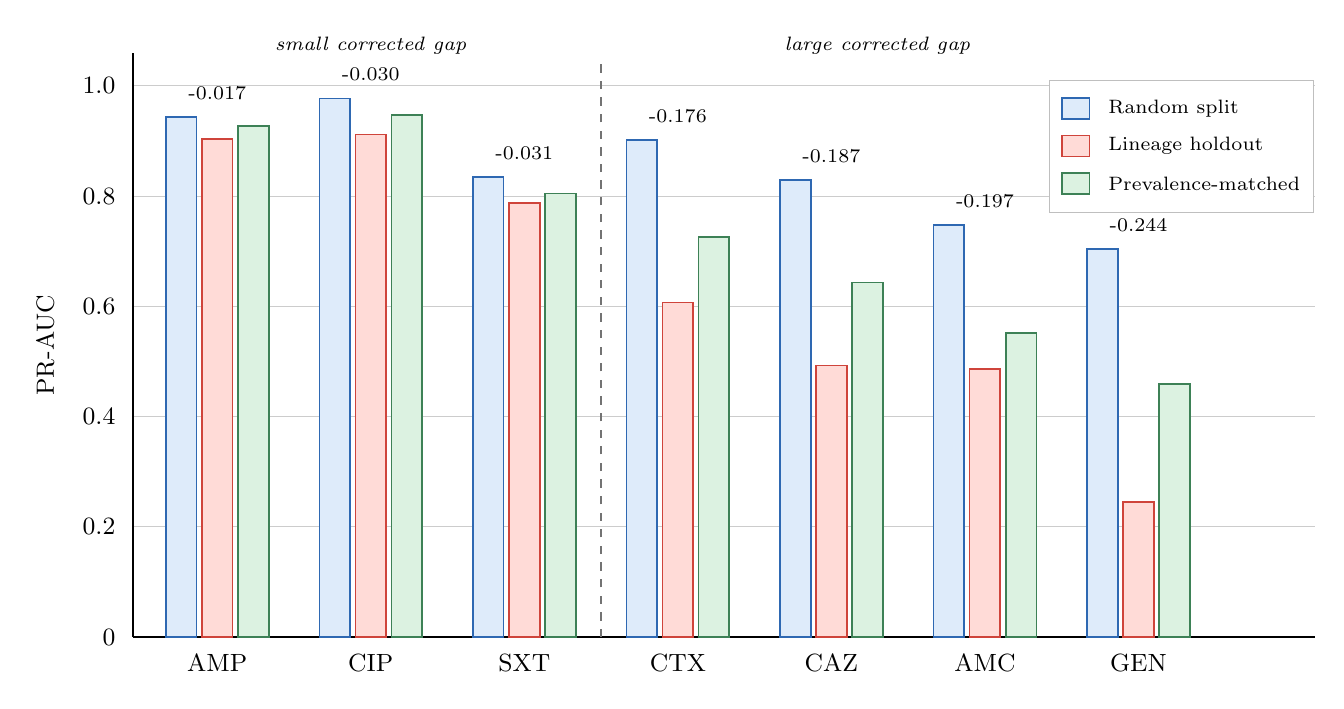
\begin{tikzpicture}[x=1.95cm, y=7.0cm]

\foreach \y in {0,0.2,0.4,0.6,0.8,1.0}{
  \draw[black!20,line width=0.4pt] (0.45,\y) -- (8.15,\y);
  \node[anchor=east,font=\small,text=black] at (0.40,\y) {\y};
}

\draw[black,line width=0.9pt] (0.45,0) -- (8.15,0);
\draw[black,line width=0.9pt] (0.45,0) -- (0.45,1.06);
\node[rotate=90,anchor=south,font=\small,text=black] at (0.00,0.53) {PR-AUC};

\foreach \i/\ab/\rnd/\hold/\mat/\gap in {%
  1/AMP/0.9440/0.9043/0.9268/{-0.017},
  2/CIP/0.9773/0.9118/0.9471/{-0.030},
  3/SXT/0.8352/0.7872/0.8046/{-0.031},
  4/CTX/0.9019/0.6073/0.7260/{-0.176},
  5/CAZ/0.8299/0.4930/0.6431/{-0.187},
  6/AMC/0.7482/0.4865/0.5513/{-0.197},
  7/GEN/0.7037/0.2457/0.4594/{-0.244}}{
    \fill[bluefill]  (\i-0.335,0) rectangle (\i-0.135,\rnd);
    \draw[blueedge,line width=0.6pt] (\i-0.335,0) rectangle (\i-0.135,\rnd);
    \fill[redfill]   (\i-0.10,0) rectangle (\i+0.10,\hold);
    \draw[rededge,line width=0.6pt] (\i-0.10,0) rectangle (\i+0.10,\hold);
    \fill[greenfill] (\i+0.135,0) rectangle (\i+0.335,\mat);
    \draw[greenedge,line width=0.6pt] (\i+0.135,0) rectangle (\i+0.335,\mat);
    \node[anchor=north,font=\small,text=black] at (\i,-0.014) {\ab};
    \node[anchor=south,font=\scriptsize,text=black] at (\i,\rnd+0.014) {\gap};
}

\draw[black!55,dashed,line width=0.8pt] (3.5,0) -- (3.5,1.04);
\node[anchor=south,font=\scriptsize\itshape,text=black,align=center]
  at (2.0,1.04) {small corrected gap};
\node[anchor=south,font=\scriptsize\itshape,text=black,align=center]
  at (5.3,1.04) {large corrected gap};

\fill[white] (6.42,0.770) rectangle (8.14,1.010);
\draw[black!25,line width=0.5pt] (6.42,0.770) rectangle (8.14,1.010);

\fill[bluefill] (6.50,0.940) rectangle (6.68,0.978);
\draw[blueedge,line width=0.6pt] (6.50,0.940) rectangle (6.68,0.978);
\node[anchor=west,font=\scriptsize,text=black] at (6.74,0.959) {Random split};

\fill[redfill] (6.50,0.872) rectangle (6.68,0.910);
\draw[rededge,line width=0.6pt] (6.50,0.872) rectangle (6.68,0.910);
\node[anchor=west,font=\scriptsize,text=black] at (6.74,0.891) {Lineage holdout};

\fill[greenfill] (6.50,0.804) rectangle (6.68,0.842);
\draw[greenedge,line width=0.6pt] (6.50,0.804) rectangle (6.68,0.842);
\node[anchor=west,font=\scriptsize,text=black] at (6.74,0.823) {Prevalence-matched};

\end{tikzpicture}
}
\caption{Random split, the sequence-type lineage holdout as measured, and the same
holdout after the test set is resampled to the training prevalence. Bars are ordered
by the prevalence-corrected gap, which is printed above each group. Three antibiotics
lose 0.017 to 0.031 once prevalence is corrected for and four lose 0.176 to 0.244,
with nothing in between. The values behind this figure are in
Table~\ref{tab:previnv}.}
\label{fig:lineage_drop}
\end{figure*}

The trend is not anywhere near homogenous and Fig.~\ref{fig:lineage_drop} renders
the split apparent: three antibiotics struggle to move, four fall sharply. Ampicillin
has a loss of only 0.040 and gentamicin has a loss of 0.458. It is the same ranking
as in Sections~\ref{sec:perfeval} and~\ref{subsec:layerabl}, only much more emphatic
here, since this is the first time a lineage has been removed as opposed to
reshuffled. The third bar in each group takes the prevalence effect out, and the rest
of this subsection explains what that means.

There are two objections to be met before all this can be credited. One is that a
failure to generalise is not the only way a drop this large can occur, it can also be
caused by near-duplicate strains. On this split zero of the 1{,}045 test strains had
a close match in training, using the same nearest-neighbour scan described in
Section~\ref{sec:statanalysis}, which found 47 such strains on the random split. The
middle column of the table demonstrates this for the phylogroup-stratified split:
four antibiotics outperform the random split and none declines by more than 0.022,
which is not the behaviour of a split that truly withholds a lineage. The second
objection does need correcting for: the holdout downwardly shifts the test-set
resistance prevalence for each antibiotic by between 2.5 and 12.1 percentage points;
gentamicin has only 38 resistant strains left. That has to be distinguished from the
drop before the drop can be interpreted as a loss of skill.

An unskilled classifier has an expected PR-AUC equal to the prevalence of the
positive class. This means that the whole scale on which PR-AUC is judged moves with
prevalence. A test partition containing fewer resistant strains will therefore score
lower even if the model ranks the strains in the same order as before. We refer to
this as the no-skill baseline rather than a floor, because a poor enough classifier
can still score below it. The opposite extreme is gentamicin, with only 38 resistant
in its holdout test set, a prevalence of 4.2\% as compared to 14.6\% in
training.

We directly measured the size of this effect. We repeatedly subsampled the
susceptible strains in the holdout test set to obtain the same prevalence as the
training set and recomputed PR-AUC on the same saved predictions for each antibiotic.
No model was re-trained and no resistant strain was abandoned.
Table~\ref{tab:previnv} presents mean over 2{,}000 resampling rounds with 95\%
interval and area under the receiver operating characteristic curve (ROC-AUC) with
no-skill value of 0.5 irrespective of prevalence.

\begin{table*}[!tb]
\caption{The lineage holdout with the prevalence effect removed. The
prevalence-matched column resamples the holdout test set to the training prevalence;
the final column is the resulting gap against the random split.}
\label{tab:previnv}
\centering
\small
\setlength{\tabcolsep}{5pt}
\renewcommand{\arraystretch}{1.05}
\begin{tabular}{|l|r|r|l|r|r|}
\hline
\rowcolor{headgrey}
\textbf{Antibiotic} & \textbf{Random split} & \textbf{Holdout, as measured} & \textbf{Holdout, prevalence-matched} & \textbf{ROC-AUC} & \textbf{Adjusted gap} \\ \hline
AMP & 0.9440 & 0.9043 & 0.9268 \;[0.918, 0.938] & 0.9257 & $\mathbf{-0.017}$ \\ \hline
CIP & 0.9773 & 0.9118 & 0.9471 \;[0.926, 0.967] & 0.9739 & $-0.030$ \\ \hline
SXT & 0.8352 & 0.7872 & 0.8046 \;[0.792, 0.823] & 0.9038 & $-0.031$ \\ \hline\hline
CTX & 0.9019 & 0.6073 & 0.7260 \;[0.687, 0.766] & 0.8838 & $-0.176$ \\ \hline
CAZ & 0.8299 & 0.4930 & 0.6431 \;[0.600, 0.679] & 0.7878 & $-0.187$ \\ \hline
AMC & 0.7482 & 0.4865 & 0.5513 \;[0.529, 0.584] & 0.6894 & $-0.197$ \\ \hline
GEN & 0.7037 & 0.2457 & 0.4594 \;[0.398, 0.511] & 0.7426 & $\mathbf{-0.244}$ \\ \hline
\rowcolor{oursblue}
\textbf{Average} & \textbf{0.8486} & \textbf{0.6337} & \textbf{0.7226} & \textbf{0.8439} & $\mathbf{-0.126}$ \\ \hline
\end{tabular}
\renewcommand{\arraystretch}{1.0}
\vspace{0.4em}

\noindent\footnotesize\textit{Note:} Once prevalence is corrected for, ampicillin's true gap is
$-0.017$, near nothing, against gentamicin's $-0.244$; the average true gap of $-0.126$ is still
well below the raw 0.215 gap the uncorrected numbers would suggest. Bold marks the extreme
values in a column, best and worst alike.
\end{table*}

Only about two-fifths of the headline drop is a prevalence effect. Average PR-AUC
falls from 0.8486 (random split) to 0.7226 when prevalence is fixed, a difference of
0.126, instead of 0.6337, a difference of 0.215, as the raw holdout values would have
indicated. As its own ROC-AUC of 0.7426 already indicated, gentamicin is the one that
most recovers, and its PR-AUC increases from 0.2457 to 0.4594: the model had not
ceased to rank resistant strains above susceptible strains, it has merely been forced
to do so on a test set where only one in twenty-four strains is resistant.

Adjusting the prevalence does not remove the discovery, instead it clarifies it. The
seven antibiotics remain divided into the same two categories, but even more distant
relative to each other. Ampicillin, ciprofloxacin and trimethoprim-sulfamethoxazole
have a loss of 0.017 to 0.031 in PR-AUC, which is near nothing, and cefotaxime,
ceftazidime, amoxicillin-clavulanate and gentamicin have a loss of 0.176 to 0.244,
and no antibiotic is in between. A model that had merely deteriorated on a more
challenging set of tests would exhibit an even distribution of losses among all seven
drugs rather than this two group divide. Amoxicillin-clavulanate is the cleanest: its
prevalence changes only by 5.9 points, thus it recovers the least of the four hard
drugs (a PR-AUC increase of 0.065, compared to gentamicin's 0.214) and also has the
lowest ROC-AUC of all seven, at 0.6894, so the least of its loss can be attributed to
prevalence at all.

Two caveats apply to this table. First, gentamicin's prevalence-matched interval is
wide, [0.398, 0.511], because it is anchored by only 38 resistant strains, so its
exact value should be read with caution even though its direction is clear. Second,
the holdout prevalence used for matching is the \textit{training} prevalence, which
is slightly higher than the random-split test set's prevalence; this makes the
comparison somewhat generous to the holdout, so the true gap may be a little larger
than the 0.126 reported above.

\subsection{Clinical Cost of the Lineage Holdout}

What the holdout costs in clinical terms is the next question.
Section~\ref{sec:perfeval} reported clinical error rates on the random split. Of
greater interest is what happens to the errors that get to a patient if the strain is
from an unfamiliar lineage. Table~\ref{tab:holdoutclin} does this, using the same
saved predictions and the same fixed threshold of 0.5, and
Fig.~\ref{fig:clinical_heatmap} does the same with the numbers arranged by
severity.

\begin{table*}[!tb]
\caption{Clinical error rates under the lineage holdout against the random split, at
a threshold of 0.5. Being within-class ratios, VME and ME are unaffected by the
prevalence shift.}
\label{tab:holdoutclin}
\centering
\small
\setlength{\tabcolsep}{5pt}
\renewcommand{\arraystretch}{1.05}
\begin{tabular}{|l|r|r|r|r|r|r|r|}
\hline
\rowcolor{headgrey}
\textbf{Antibiotic} & \textbf{Resistant in test} & \textbf{VME random} & \textbf{VME holdout} & \textbf{Increase} & \textbf{ME holdout} & \textbf{CA random} & \textbf{CA holdout} \\ \hline
CIP & 132 & 0.086 & 0.114 & $+0.028$ & 0.006 & 0.969 & 0.978 \\ \hline
AMP & 300 & 0.109 & 0.160 & $+0.051$ & 0.095 & 0.893 & 0.877 \\ \hline
SXT & 142 & 0.236 & 0.310 & $+0.074$ & 0.072 & 0.871 & 0.863 \\ \hline\hline
AMC & 145 & 0.394 & 0.710 & $+0.316$ & 0.076 & 0.804 & 0.754 \\ \hline
GEN & 38  & 0.436 & \textbf{0.868} & $+0.432$ & 0.002 & 0.934 & 0.962 \\ \hline
CAZ & 43  & 0.291 & \textbf{0.837} & $+0.546$ & 0.001 & 0.936 & 0.959 \\ \hline
CTX & 71  & 0.190 & \textbf{0.915} & $+0.725$ & 0.001 & 0.953 & 0.918 \\ \hline
\rowcolor{oursblue}
\textbf{Mean} & --- & \textbf{0.249} & \textbf{0.559} & $\mathbf{+0.310}$ & --- & --- & --- \\ \hline
\end{tabular}
\renewcommand{\arraystretch}{1.0}
\vspace{0.4em}

\noindent\footnotesize\textit{Note:} Gentamicin (0.868), ceftazidime (0.837) and cefotaxime
(0.915) all have a holdout VME above 0.83, meaning the model has effectively stopped finding
resistance for these three; the mean row averages across all seven.
\end{table*}

\begin{figure}[!tb]
\centering
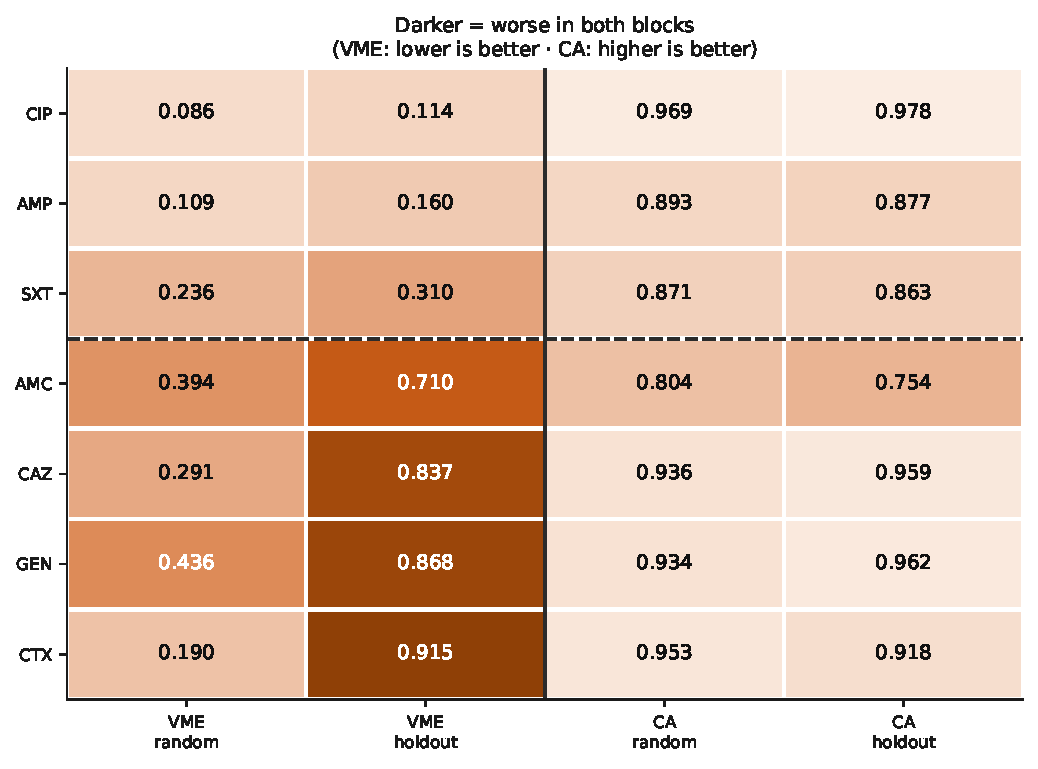
\includegraphics[width=\columnwidth]{fig_clinical_heatmap.pdf}
\caption{Very major error rate (left pair, lower is better) and categorical agreement
(right pair, higher is better), random split against lineage holdout. Drugs are
ordered by holdout VME; the dashed line marks the split between the two groups. Each
cell is annotated with its value, so the figure can be read without reference to the
colour scale.}
\label{fig:clinical_heatmap}
\end{figure}

The average very major error rate increases from 0.249 to 0.559 and for three
antibiotics, the model has completely ceased to detect resistance. It detects 6 of
the 71 cefotaxime-resistant strains, 5 of the 38 gentamicin-resistant strains and 7
of the 43 ceftazidime-resistant strains, with a major error rate of 0.001 or 0.002
for each group. That combination is the hallmark of a classifier that has collapsed
onto the majority class: it hardly ever makes a resistant prediction, so it hardly
ever makes such predictions wrongly. These numbers are more difficult to dispute than
the PR-AUC values above since VME and ME are calculated within a class and stay fixed
as the class mix varies. Prevalence-matching resamples only susceptible strains, and
very major error rate is considered to be all in the resistant category, thus cannot
be resampled. Clinical deterioration here therefore has no prevalence component, and
requires no correction before it can be believed.

The categorical agreement column demonstrates why accuracy does not drive this
research. Three antibiotics show equal or higher categorical agreement in the holdout
than in the random split, and for the other four the reduction in agreement is much
smaller than the total collapse in clinical safety alongside it. Gentamicin increases
from 0.934 to 0.962 while very major error rate doubles to 0.868; ceftazidime from
0.936 to 0.959, missing 36 of the 43 resistant strains; cefotaxime changes by just
0.035 but its very major error rate rises from 0.190 to 0.915. By the measure a
machine learning paper would use to report results, this model looks better or nearly
as good, on unseen lineages; by the measure a clinician would use, it became
unusable.

This is the third analysis to produce the same grouping. They are the same three with
the same saved predictions and test set, therefore they are complementary views but
measure different aspects of those predictions. The three antibiotics with negligible
loss in PR-AUC gain between 0.028 and 0.074 in very major error rate, and the four
with a significant loss have a gain of 0.316 to 0.725. The order within the second
group changes, as cefotaxime is worst in this group whereas gentamicin was worst
using PR-AUC, the rank within the groups is not to be overly read, but the grouping
does not change across all three analyses.

\subsection{Component Performance Under the Lineage Holdout}

The holdout also allows us to redo the component analysis of
Section~\ref{subsec:layerabl} in more difficult conditions, and
Table~\ref{tab:mlst_components} shows that the outcome alters the previous picture.

\begin{table}[!tb]
\caption{Average PR-AUC of each component of the model, under the lineage holdout.}
\label{tab:mlst_components}
\centering
\small
\setlength{\tabcolsep}{4pt}
\renewcommand{\arraystretch}{1.05}
\begin{tabular}{|l|r|}
\hline
\rowcolor{headgrey}
\textbf{Component} & \textbf{Avg PR-AUC} \\ \hline
TriLens neural arm alone (lenses with gate) & 0.472 \\ \hline
Five classical learners alone & \textbf{0.628} \\ \hline
\rowcolor{oursblue}
Full hybrid model & \textbf{0.634} \\ \hline
\end{tabular}
\renewcommand{\arraystretch}{1.0}
\vspace{0.4em}

\noindent\footnotesize\textit{Note:} The classical learners alone reach 0.628, close to the full
hybrid model's 0.634 under this harder split, meaning the neural lenses add almost nothing here.
The 0.634 in the last row is the 0.6337 reported to four decimal places in
Table~\ref{tab:mlst_per_ab}. The 0.628 in the middle row is the five base
learners \emph{stacked}, and is a different quantity from the 0.6299 of
Table~\ref{tab:baselines}, which is the single strongest learner on its own: under
this split the stacking layer recovers slightly less than its own best member
already had.
\end{table}

The neural arm alone, that is the three lenses with the gate, scored 0.781 on the
random split. It plummets to 0.472 here, when tested on truly unseen lineages; this
represented a much larger decline compared to what the classical learners achieve on
their own (0.628), nearly matching the full hybrid model (0.634). The classical
learners do nearly all of the work under a true test of generalisation and the neural
lenses add almost nothing. It is a stronger form of what
Section~\ref{subsec:layerabl} already indicated: the gap between the two arms is
0.156, and the fused model only recovers 0.006 of it. But this was not a case where
some other deep learning design would have generalised better; TabNet reran on this
split averages 0.326, worse than our neural lenses on their own and well below the
classical learners. Gradient-boosted trees on gene-level features are the best method
we identified on this dataset and under this type of test.

\subsection{Transfer to an Independent Collection}

The downside on unseen lineages gives one an obvious next question: does it work at
all on a different set of strains? The two datasets do not have a shared feature
vector as Arcadia uses the pan-genome reference with 535{,}000 variant positions and
Giessen uses a single reference with approximately 60{,}000 variant positions. We
rather trained the classical stacking part of the pipeline on Giessen with the same
protocol and hyperparameters. The three neural lenses require feature shapes only the
pan-genome view can provide and thus are not included in this comparison; and four
antibiotics are in common to both collections.

\begin{table}[!tb]
\caption{The classical stacking half of the pipeline, trained independently on a
second collection. Neither column is the full TriLens model.}
\label{tab:giessen_transfer}
\centering
\small
\setlength{\tabcolsep}{4pt}
\renewcommand{\arraystretch}{1.05}
\begin{tabular}{|l|r|r|r|}
\hline
\rowcolor{headgrey}
\textbf{Antibiotic} & \textbf{Arcadia} & \textbf{Giessen} & \textbf{Retention} \\ \hline
CIP & 0.9773 & 0.9868 & \textbf{101.0\%} \\ \hline
CAZ & 0.8299 & 0.7775 & 93.7\% \\ \hline
CTX & 0.9019 & 0.7876 & 87.3\% \\ \hline
GEN & 0.7037 & 0.5480 & \textbf{77.9\%} \\ \hline
\rowcolor{oursblue}
\textbf{Average} & \textbf{0.8532} & \textbf{0.7750} & \textbf{90.0\%} \\ \hline
\end{tabular}
\renewcommand{\arraystretch}{1.0}
\vspace{0.4em}

\noindent\footnotesize\textit{Note:} Ciprofloxacin's apparent 101.0\% retention is the highest in
the table and gentamicin's 77.9\% the lowest, matching the ordering seen under the lineage
holdout. As the text below explains, these retention figures are inflated by Giessen's higher
prevalence rather than by genuinely better performance. The average retention of 90.0\% is
the mean of the four per-drug ratios; the ratio of the two column means is 90.8\%. Bold marks
the extreme values in a column, best and worst alike.
\end{table}

The approach keeps about 90\% of its performance on a genomically different
collection. It is not zero-shot transfer, in that the model was retrained; what it
demonstrates is that our design decisions are not optimized to the specifics of a
single dataset.

There is one caveat here, the same one this section raises so many times elsewhere.
Section~\ref{subsec:prevmatch} holds that PR-AUC cannot be compared across partitions
with differing prevalence, and the two collections differ significantly in
prevalence. In Arcadia, the resistance of ciprofloxacin stands at 0.228 as compared
to 0.452 in Giessen. Cefotaxime is 0.152 resistant in Arcadia as compared to 0.443 in
Giessen. In Arcadia, ceftazidime is 0.131 resistant against 0.341 in Giessen.
Gentamicin has a resistance of 0.118 in Arcadia compared to 0.232 in Giessen. In
Giessen, every drug's no-skill baseline is about twice to three times Arcadia's,
before the model is credited with any skill at all. So the retention percentages are
misleading by this difference in baselines, not by any actual improvement, and
perhaps the most transparent example is ciprofloxacin whose apparent 101\% indicates
that the model is marginally better on Giessen, but what really happened is that
Giessen made the task marginally easier. The bias cannot be eradicated, because
prevalence-matching would require both collections to be resampled to an identical
reference, and the 81-strain Giessen test partition is too small to survive that
exercise. The weaker argument is the one we will justify from this table: that the
recipe reconstructs and does not fall apart, not that performance is maintained to
within ten percent of its original extent. The interesting part is the per-antibiotic
pattern. Ciprofloxacin retains most of its performance and gentamicin only 77.9\% of
its own, the same order as under the lineage holdout, though reached by an entirely
different route.

\subsection{Marker Genes and Their Annotation}
\label{subsec:markers}

We obtained the most impactful genes based on two sources: the weights of attention
within the three neural lenses, and SHAP values obtained with the five classical base
learners. This provided 1{,}138 marker genes in total which covered all antibiotics.
Their Prokka \cite{seemann2014prokka} locus tags alone do not provide us with any
information, so we aligned them with the eggNOG \cite{huertacepas2019eggnog}
functional annotation released with the Arcadia dataset. We were
successful in annotating 889 of the 1{,}138 markers, or 78.1\%, with the others
having no corresponding match and indicating them as not annotated instead of making
a best guess. Eight of the annotated markers were known genes involved in
antimicrobial resistance: \textit{gyrA}, \textit{parC}, the two target genes where
point mutations result in fluoroquinolone resistance; \textit{emrB}, \textit{mdtC},
\textit{mdtD} and \textit{mdtO}, which are parts of multidrug efflux pumps;
\textit{cusA}, which belongs to the copper and silver efflux system and is therefore
a heavy-metal rather than a drug transporter, so we count it as an efflux marker but
not as direct evidence of an antibiotic mechanism; and one additional gene annotated
as a beta-lactamase.

The genuine result is in finding \textit{gyrA} and \textit{parC} and it is more
significant following the lineage holdout than ever. These are the textbook
objectives of ciprofloxacin resistance and ciprofloxacin was the very antibiotic that
did not succumb to the holdout most, dropping only 0.030 when prevalence is held
constant, as compared to other antibiotics that dropped up to 0.244. A model based on
an actual, conceptually clear mutation should be transferred to a new lineage and
that is what we observe.

A single detail is more important than the list of genes. The eight resistance genes
were all the result of the SHAP analysis of the classical learners. None was a result
of attention weights of the three neural lenses, although 420 out of the 1{,}138
markers were selected out of those lenses.

Two things besides a real failure could bring about that zero, and we tested each of
them. The first is annotation coverage, as an eggNOG file lacks a gene and there is
no way to identify it as a resistance gene no matter how significant the model
considered it to be. The two of three lenses are eliminated by coverage: each of 140
markers contained in the Cross-Antibiotic Context Module was annotated, and 97.9\% of
markers in the Motif Pattern Encoder, but neither generated a single resistance gene.
The weaker case is the Gene Feature Attention Module at 61.4\%, which is important as
it is the lens the gate is most dependent on, thus the view that our model believes
is best will be the one that we can reasonably interpret least. The second option is
that twenty genes per lens per drug is too small a window. We therefore repeated the
annotation on the top 100 genes instead of the top 20, a fivefold widening of the
window, which raised coverage to 79.3\%. It also did not recover any resistance gene,
so the zero is not an artefact of the depth at which the ranked list was truncated.

Another measurement can be used to explain why. The variant sweep that followed the
final lens design concentrated focus on the 5{,}000 selected genes instead of the
entire catalogue of 32{,}441 genes, thus the maximum attainable entropy there was
$\ln 5{,}000 \approx 8.52$, not the $\ln 32{,}441 \approx 10.39$ of the full set.
Compared against this lower ceiling, attention entropy remains at 8.51 for
trimethoprim-sulfamethoxazole, effectively at ceiling, and above 7.79 for
amoxicillin-clavulanate, gentamicin, cefotaxime and ceftazidime, still at or within
ten percent of it. When the attention mass of the five drugs is at the most not even
one percent of the total mass, in any case, and when ninety percent of it is
distributed amongst two or four thousand genes, the pooling layer has virtually broken
down into a mere mean. Only ampicillin and ciprofloxacin exhibit real concentration,
with entropies 5.34 and 5.46 with just under twenty genes exceeding one percent each,
and we by no means attribute biology to even that, since another pooling function
tested in a separate sweep concentrated on another group of drugs, indicating the
pattern follows the architecture and not the resistance mechanism.

What it does focus on is still informative. Each gene in the pan genome has a locus
tag that indicates which of the assemblies the gene was called from, providing an
inexpensive method to determine which of the attended genes are sampled or from across
the pan genome. For the Gene Feature Attention Module they are not: for each of the
seven antibiotics, the top genes by this module were concentrated in a single assembly
between 12 times that assembly's fraction in the catalogue and 23 times: median was
16.4. Those counts are less informative because they represent a small number of genes
per antibiotic, only genes with an assembly tag can be counted and that counts less
than a dozen genes in total, so we read the ratio more as an indicator of the
direction of the lens than as a formal test.

An obvious objection is that this is simply an artefact of how pan-genome clusters are
named, as each cluster takes the tag of whichever assembly represented it, and a well
represented assembly would then swamp any list by arithmetic. There are two reasons
why not to think so. The assembly the lens focuses on provides merely 3.3\% of the
catalogue, therefore, abundance can not account for a twenty-fold preference. And the
other two lenses do only just what the artefact explanation would predict: both focus
on the \textit{most} populous tag they are reading, at an enrichment of only 1.6 to
2.1, so that we do not report them as a discovery.

\subsection{Ablation of Strain Conditioning in Lens B}
\label{subsec:strainablation}

These above are what attention still cannot do. They are, however, much better than
the results obtained via a direct application of gated attention pooling on this
input, and this difference is one of the design contributions of this work: it is the
only area where we changed the mechanism itself rather than the data it reads from.
Section~\ref{subsec:lensB} and
Equations~\eqref{eq:expertB_ctx}--\eqref{eq:expertB_score} set out the argument in
full: on a presence-and-absence vector the standard gated-attention score becomes
simply that gene's embedding, and is thus identical for all strains that carry that
gene, and conditioning it on the mean embedding of the genes the strain actually
carries restores per-sample behaviour. As this reasoning predicts a behaviour, we
evaluated it in an ablation, training the model in both directions using the same
seeds, folds, splits and hyperparameters, changing only this single term.
Table~\ref{tab:attnfix} reports the effect.

\begin{table*}[!tb]
\caption{Ablation of strain conditioning in the Gene Feature Attention Module.
Everything but this one term is identical, and the ``Fixed'' column is the delivered
model reported everywhere else. The reference column gives the comparison value the
row is read against, and is not part of the ablation.}
\label{tab:attnfix}
\centering
\small
\setlength{\tabcolsep}{5pt}
\renewcommand{\arraystretch}{1.05}
\begin{tabular}{|>{\raggedright\arraybackslash}p{5.0cm}|r|r|r|>{\raggedright\arraybackslash}p{3.0cm}|}
\hline
\rowcolor{headgrey}
\textbf{Measure} & \textbf{Standard} & \textbf{Fixed} & \textbf{Change} & \textbf{Reference} \\ \hline
\multicolumn{5}{|l|}{\textit{Predictive performance}} \\ \hline
Random split, full stack & 0.8462 & 0.8486 & $+0.0024$ & --- \\ \hline
Phylogroup-stratified split & 0.8519 & 0.8531 & $+0.0012$ & --- \\ \hline
Lineage holdout, full stack & 0.6300 & 0.6337 & $+0.0037$ & --- \\ \hline
Lineage holdout, classical alone & 0.628 & 0.628 & $\pm 0$ & --- \\ \hline
\rowcolor{oursblue}
\textbf{Holdout, neural lenses alone} & \textbf{0.437} & \textbf{0.472} & $\mathbf{+0.035}$ & --- \\ \hline
\multicolumn{5}{|l|}{\textit{Clinical safety and interpretability}} \\ \hline
Mean very major error rate & 0.257 & 0.249 & $-0.008$ & --- \\ \hline
Resistance genes by attention & 0 & \textbf{1} & $+1$ & SHAP 8 \\ \hline
$U_{res}$ of attended genes & 0.0192 & \textbf{0.0419} & $+0.0227$ & SHAP 0.0473 \\ \hline
$U_{ST}$ of attended genes & 0.3123 & 0.3569 & $+0.0446$ & random 0.5390 \\ \hline
Enrichment on one assembly & $16.4\times$ & $9.0\times$ & $-7.4\times$ & --- \\ \hline
\end{tabular}
\renewcommand{\arraystretch}{1.0}
\vspace{0.4em}

\noindent\footnotesize\textit{Note:} Under the lineage holdout, the neural lenses alone gain
0.035 from strain-conditioning, an order of magnitude more than the 0.0024 it buys on the random
split; the two interpretability rows move with it, from zero resistance genes recovered to one,
and $U_{res}$ nearly doubling from 0.0192 to 0.0419. $U_{ST}$ is the one measure that
moves the wrong way, as the text below discusses.
\end{table*}

\begin{figure}[!tb]
\centering
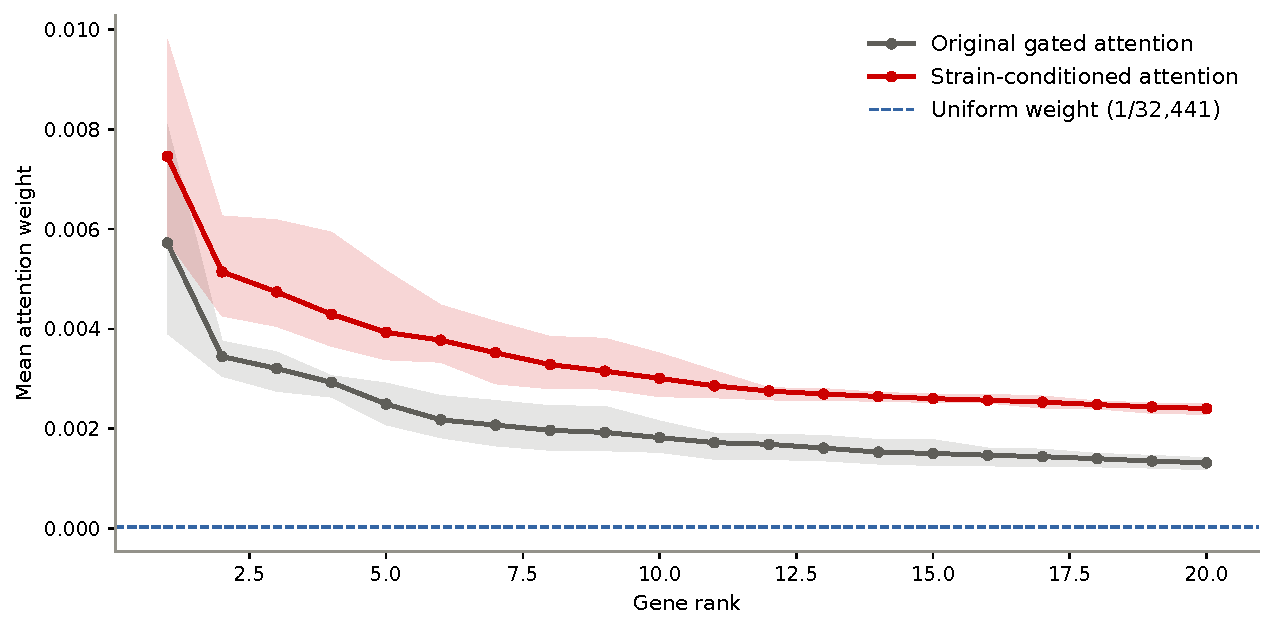
\includegraphics[width=\columnwidth]{fig_attention_concentration.pdf}
\caption{Mean attention weight against gene rank in the Gene Feature Attention
Module, averaged over the seven antibiotics, before and after strain conditioning.
The shaded band is the full minimum-to-maximum range across the seven antibiotics at
each rank, and the dashed line is the weight a
uniform distribution would place on every one of the 32{,}441 genes.}
\label{fig:attention_concentration}
\end{figure}

Three of the four interpretability measures go in the expected direction, and one
does not. As Fig.~\ref{fig:attention_concentration} shows, the strain-conditioned
lens concentrates more weight on its highest-ranked genes at every rank, and the
resistance information of the attended genes more than doubles from 0.0192 to 0.0419,
which is 89\% of the SHAP-selected genes on average, and greater than them on five
out of seven antibiotics. The focus on a single assembly drops from 16.4-fold to
9.0-fold and three out of the seven drugs are no longer significant at the 5\%
threshold, and the number of independent source assemblies among the attended genes
almost doubles, so the provenance signature is mostly diluted.

The exception is $U_{ST}$, which rises from 0.3123 to 0.3569. By the convention of
Fig.~\ref{fig:lineage_marker}, where a lower value means a gene set is less
determined by lineage, that is a movement in the wrong direction, and we report it as
such rather than presenting the ablation as uniformly favourable. Both values remain well
below the 0.5390 of a random gene, so the attended set is still less
lineage-determined than the pan-genome at large, but strain conditioning buys its
extra resistance information at the cost of some of that margin. The two quantities
are not independent: genes that carry resistance information in this collection are
also, on average, more lineage-structured, which is the same coupling that
Section~\ref{sec:discussion} identifies as the reason four of the seven antibiotics
fail to transfer. We therefore read the pair together, as a trade rather than as a
clean improvement.

The rows of performance are not as plain as they appear at the first sight as the term
buys practically nothing where it can be measured with ease and much where it is
needed. Strain conditioning is worth almost nothing where it is easiest to measure:
$+0.0024$ on the random split, and $+0.0037$ on the full stack under the lineage
holdout. It is worth an order of magnitude more, $+0.035$, on the neural lenses alone
under that same holdout, while the classical learners do not move at all and stay at
0.628. An ablation run only on the random split would have hidden this completely. The
degenerate scoring function was costing the neural arm most of what it lost anywhere,
on precisely the split this research is interested in, and the classical arm was strong
enough that none of that loss ever showed in the headline number.

Our most interesting change is the one which we have not tuned for. The attention
restores MFCAOJAD\_04226, a beta-lactamase, with the score conditioned to the presence
of the strain, and selectively recovers it with ampicillin and
amoxicillin-clavulanate, the two penicillins in our panel and the two drugs which a
beta-lactamase can explain being resistant to. It is the locus tag that SHAP had
already determined in the classical learners and thus, two attribution paths that
previously disagreed on all points now converge on a single gene, independently. We do
not exaggerate this: it is a single gene per hundred genes tested each lens per drug,
it is ranked 19 and 20 instead of first, and \textit{gyrA} and \textit{parC} have not
appeared in the attention rankings.

One boundary applies. This is information on the presence and absence vector for
attention, and is specific to that input, not to attention pooling in general. What
generalises is that the diagnostic is an attention mechanism whose scores do not change
across samples, which means that we cannot obtain a per-sample explanation and we can
figure out that fact in minutes, without retraining anything. We computed the fraction
of presence-absence entropy, $U_{ST}(g) = I(g;\mathrm{ST})/H(g)$, which is equal to 1
if a gene's presence is completely attributed to its lineage and 0 if it says nothing
about the gene's lineage. In Table~\ref{tab:umark} the selected genes are compared with
the genes attended and to 500 random selections of equal size.

\begin{table}[!tb]
\caption{How much of each gene set is explained by lineage ($U_{ST}$) and by
resistance ($U_{res}$), over the top twenty genes per antibiotic. The attention row is
the standard formulation; the delivered strain-conditioned lens reaches 0.357 and
0.0419.}
\label{tab:umark}
\centering
\small
\setlength{\tabcolsep}{4pt}
\renewcommand{\arraystretch}{1.05}
\begin{tabular}{|>{\raggedright\arraybackslash}p{2.6cm}|r|r|r|r|}
\hline
\rowcolor{headgrey}
\textbf{Gene set} & \textbf{$U_{ST}$} & \textbf{vs.\ rand.} & \textbf{$U_{res}$} & \textbf{vs.\ attn.} \\ \hline
Random genes (500 draws) & 0.539 & N/A & N/A & N/A \\ \hline
SHAP, classical learners & 0.375 & $0.70\times$ & \textbf{0.0473} & $2.5\times$ \\ \hline
Attention, Lens B & \textbf{0.312} & $0.58\times$ & \textbf{0.0192} & N/A \\ \hline
\end{tabular}
\renewcommand{\arraystretch}{1.0}
\vspace{0.4em}

\noindent\footnotesize\textit{Note:} Attention's $U_{ST}$ of 0.312 is lower than a random gene's
0.539, so the attended genes are not a lineage marker; its $U_{res}$ of 0.0192 is less than half
of SHAP's 0.0473, so they carry far less resistance information than the genes the classical
learners select.
\end{table}

\begin{figure}[!tb]
\centering
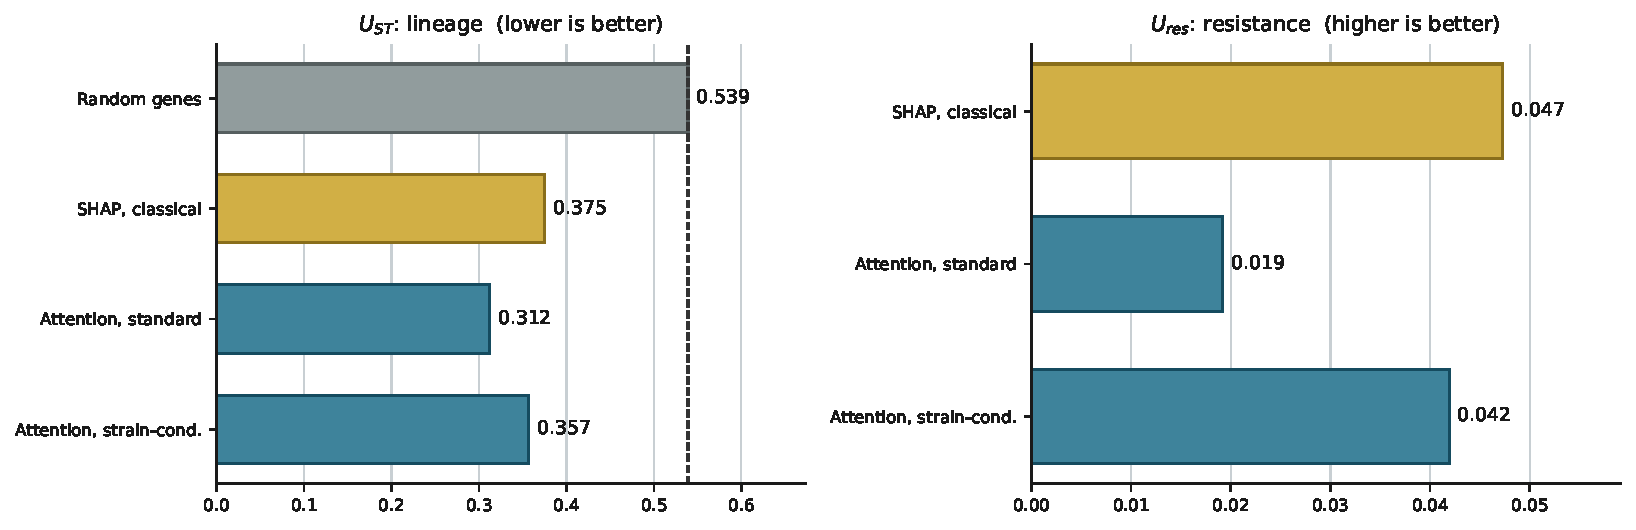
\includegraphics[width=\columnwidth]{fig_lineage_marker.pdf}
\caption{The attended gene sets against SHAP and against random draws, on both
measures. Lower is better on the left, higher is better on the right.}
\label{fig:lineage_marker}
\end{figure}

There are two things that follow, both depicted in Fig.~\ref{fig:lineage_marker}.
The first is not a feature of our model itself, but of the data: the presence-absence
pattern of a random gene from this pan-genome is explained to 54\% by sequence type.
Such strongly lineage-structured content of \textit{E. coli} accessory genes is the
most obvious single reason why a lineage-sensitive split was required in the first
place.

The second one is that the genes attended are not a lineage marker. They are
\textit{less} lineage-determined by the standard formulation, at 0.312; and by the
delivered formulation, at 0.357, than a random gene; and nothing in the 500 random
draws was below them. Nor do they hold much information of resistance: their $U_{res}$
of 0.0192 is the lowest of the three sets, about half the 0.0473 that the genes SHAP
chooses do, and even the strain-conditioned version is only 0.0419. It is not the lens
that read the wrong thing but the lens that read hardly anything. The useful part is
the comparison with SHAP in that both sets of genes were selected on the same trained
pipeline on the same features: the classical side picks genes with two and a half times
more resistance information. This matches the result reported in
Section~\ref{subsec:prevmatch}, where the neural lenses alone under the lineage holdout
remain at 0.472 while the classical learners remain at 0.628. It is the same learners
who generalise that are also the ones which pick the more informative genes.

This conflict does not exist solely on the neural side. In the classical arm, the two
attribution modes also struggle to agree to a great degree. When the top twenty genes
ranked by XGBoost gain are compared with the top twenty genes ranked by SHAP, by each
antibiotic and by both sets of classical features, the Jaccard overlap ranges between
0.053 and 0.212, with an average of 0.11 on the gene-aggregated features and 0.17 on
the raw SNP features, so at best only four to six genes out of twenty will be shared
between the two lists. The rank correlation is not so good: Spearman is negative with
all seven antibiotics, between $-0.04$ and $-0.53$. That figure needs a qualification
before it is read as a disagreement about the model. It is computed over the union of
the two top-twenty lists, not over the full ranking of 5{,}000 genes, so it describes
only how the two methods order the handful of genes that at least one of them already
considers important. Over so short and so truncated a range a correlation is unstable
and its sign carries little weight; what the negative values establish is the absence
of agreement at the top of the ranking, not the presence of a systematic inversion. The
Jaccard figures are the more reliable of the two statistics for the same reason. Even
on the weaker reading, the results of two methods of attributing to the same trained
model are not expected to overlap this little, and hence neither can be taken as the
interpretation of the model itself. The findings of the
gene level, then, are reported as leads but not settled biology, such as the eight
resistance genes above, which are informative because they are all in agreement with
independently determined biology but not because the attribution method has ascertained
them.

% =====================================================================
\section{Discussion}
\label{sec:discussion}
% =====================================================================

\subsection{Mechanism Against Population Structure}

With the corrected split in hand, the pattern across antibiotics becomes much clearer
than it was before. The most obvious example of a learnt real mechanism is
ciprofloxacin. It also decays with a 0.030 loss when prevalence is held fixed and its
two known resistance genes are in our annotated markers. \textit{E. coli} resistance
to fluoroquinolone is typically due to point mutations in these genes: a small,
precisely defined signal, and precisely that which a model can learn once, and then
recall in an unrelated isolate.

Gentamicin is the opposite case. When prevalence is fixed it still loses 0.244, the
largest gap of the seven, and no aminoglycoside-resistance gene feature enters into
the final model. The gentamicin resistance often comes on plasmid and mobile element
genes and is transferred in a lineage specific manner far more than it is across
lineages, and does not assemble well in a pan-genome built this way with this dataset.
The model has learned essentially which lineage a strain belongs to, not which gene it
harbors. Lastly, ceftazidime and cefotaxime, which have losses of 0.187 and 0.176,
respectively, potentially share overlapping mobile beta-lactamase elements.

This account is not fully separable from a decision made in our own pipeline, and we
will not present it as though it were. Section~\ref{sec:datatransform} sets missing
genotype calls to the reference allele, following the authoring group, and notes there
that a call fails most often on plasmids and other mobile elements that assemble poorly
from short reads. That is the same set of loci on which the four difficult antibiotics
depend. The biological reading above and the artefact of our imputation therefore
predict the identical outcome on the identical drugs, and nothing in the experiments
reported here distinguishes them. Two observations keep the biological reading in play:
amoxicillin-clavulanate, whose usual mechanism is a change in expression level rather
than the acquisition of a gene, fails in the same group despite not depending on
assembly at all; and the ordering of the seven drugs reproduces under the independent
Giessen collection, which was called against a different reference. Neither is decisive.
Repeating the pipeline with missing calls masked rather than imputed would separate the
two, costs nothing but compute, and is listed in Section~\ref{sec:conclusion} as
future work. Until it is done, the mechanism account should be read as the more probable
of two live explanations rather than as an established one.

The most obvious example of another failure is amoxicillin-clavulanate that loses
0.197. The expression of more enzyme or release of a membrane channel, changes in
degree, rather than changes in which genes are expressed, are often the basis of its
resistance. This type of resistance can never be easily overcome by our
presence-and-absence lens, which bears most of the weight of the entire gate during
the course of this research, and therefore this type of resistance was never going to
be easy to capture in our design.

All this does not make the model useless. It is efficient on simple, well known
mechanisms and inefficient on resistance as carried by mobile, plasmid-borne elements
or by low level changes in gene expression. This is a specific, falsifiable claim
about the current state of genomic AMR prediction, and a more useful conclusion than
an average score would have been.

\subsection{Answers to the Research Questions}

Taking the five research questions of Section~\ref{sec:intro} in turn.

\textbf{RQ1.} TriLens-MoE-Stack achieved an average PR-AUC of 0.849 on the random
split, the highest in Table~\ref{tab:baselines}. It is ahead of every external
baseline and ahead of its strongest component on five of the seven antibiotics. But
its margin over the best single classical learner is only 0.009, which falls within
the bootstrap intervals and is of the size that seed variation alone could produce,
since every model here was trained once (Section~\ref{sec:statanalysis}). The claim
that can be defended is therefore the weaker one: nothing simpler beats it, rather
than that it beats everything simpler.

\textbf{RQ2.} Each component has its contribution to make, and the classical arm has
the greatest: the addition of the gate is 0.035 and the classical step of stacking
0.068 to the random split (Section~\ref{subsec:layerabl}). According to the lineage
holdout, the classical learners are the only ones to hit 0.628, compared to the entire
model 0.634, and the neural lenses are the only ones to hit 0.472, so on truly new
lineages, the neural side contributes almost nothing. The 0.068 that stacking adds is
comfortably larger than the interval widths of Section~\ref{sec:statanalysis}; the
0.035 that the gate adds is not, and is reported as a direction rather than as a
quantity.

\textbf{RQ3.} Answered in the negative but a diagnosis was made. The gate weights can
be read but are inconsistent with the prediction of the design, diverting
ciprofloxacin off of the motif lens designed to receive it. The attention weights
reclaim a single known resistance gene in 420 markers, eight in SHAP on the classical
arm. Section~\ref{subsec:strainablation} shows that this failure can be attributed
to a particular and remediable attribute of the lens, an attribute more valuable
than a positive answer we cannot justify.

\textbf{RQ4.} A blend with relative proportions that change dramatically by
antibiotic. Coarse phylogroup membership has virtually no signal on its own (0.291),
and gene annotation recovers \textit{gyrA} and \textit{parC} unprompted, but the
prevalence-corrected holdout indicates that finescale relatedness has a lot: three
drugs lose 0.017 to 0.031 and four lose 0.176 to 0.244, with no results in between.
There is no one answer to RQ4, just a per-antibiotic one.

\textbf{RQ5.} Partially incomplete and uneven generalisation. Average performance
drops from 0.849 to 0.634 (or 0.723 after correcting for the prevalence shift) and
leftover duplicates are ruled out by a near-duplicate scan. It holds reasonably well
for antibiotics with a simple well-understood mechanism and badly for antibiotics
whose resistance is linked to mobile genetic elements or to changes in gene
expression.

% =====================================================================
\section{Conclusion}
\label{sec:conclusion}
% =====================================================================

A genomic resistance model can look excellent on paper and still be measuring the
wrong thing. That doubt is where this research started. The question we set out to
answer was how much of the score comes from real biological patterns, and how much
comes from similarities between related strains. We had to have a powerful model in
order to test this fairly. TriLens-MoE-Stack was able to obtain an average PR-AUC of
0.849 on the random split, the best score of all the models tested. Against every
method from outside this work the lead is clear: 0.045 over the PCA gradient-boosting
model this project began with, 0.154 over TabNet, and 0.557 over the null model, and
on three of the seven antibiotics the score clears the upper bound of that baseline's
confidence interval. Against its own strongest component the margin is 0.009, which is
what an ablation is expected to show once the best part is already in place. Then
whole sequence types were removed from training and no test strain had a close
neighbour in the training set. The average PR-AUC decreased to 0.634. A portion of
this decrease was due to a decreased fraction of resistant strains in the holdout set
which has a direct impact on PR-AUC. This change was corrected, and the score was
0.723. The actual difference was not 0.215 but 0.126. Also, the decline in performance
was quite distinct across antibiotics. Three antibiotics lost only 0.017 to 0.031,
while four lost 0.176 to 0.244. This stark division indicates that the resistance
associated with the stable biological processes can be transferred to new lineages,
whereas the patterns primarily depending on the ancestry are not very transferable.
When the classical part of the pipeline was rebuilt on a second dataset, it kept about
90\% of its earlier performance. That figure applies to the classical stacking half
alone, since the neural lenses need a feature space the second collection does not
provide, and Giessen's higher resistance prevalence raises the floor against which
PR-AUC is read, so the number is better treated as evidence that the recipe
reconstructs than as a measurement of how much accuracy survives. What it indicates is
that the design decisions of that half are not tied to the specific characteristics of
a single dataset.

However, there are also significant limitations to these results. None of the
antibiotics passed both CLSI error limits, so the error rates stay above the level
those limits set. That weakness is concentrated in a few drugs rather than spread
across the panel. For ciprofloxacin and ampicillin the model reaches 0.9773 and 0.9440
on the random split, and still holds 0.9118 and 0.9043 when every close relative is
removed from training. The lineage holdout led to a higher share of resistant strains
being incorrectly classified as susceptible (0.249 to 0.559), although the
accuracy-like measure did not change significantly. This distinction is important
since the accuracy-like measure is commonly reported in the majority of studies and it
may conceal severe clinical errors. The results of the interpretation were also not
entirely consistent. In the attention weights, only one known resistance gene was
identified whereas eight were identified using post-hoc attribution to classical
learners. Thus the gene-level results should be viewed as potential leads rather than
established biological truths. There is also a definite limit to the gene presence and
absence lens. It is able to identify the presence of a gene, but not the level of gene
expression. This may account for amoxicillin-clavulanate being the most difficult
antibiotic during the study. One more limitation arises from the stratified split that
is based on the phylogroup labels. These labels were extracted from an unreferenced
lookup table for 57 sequence types and we were not able to verify the original source
of that table; calling the phylogroup directly from each genome with an established
\textit{in silico} typing tool \cite{beghain2018clermontyping} would put that split on
a documented footing.

Four further limitations bound what the numbers above can carry. First, every model
was trained once, under a single seed, so the intervals we report cover test-set
sampling but not training variability, and the smallest differences in
Tables~\ref{tab:baselines} and~\ref{tab:attnfix} should not be read as established
effects. Second, the lineage-only and PCA baselines were evaluated on the random split
but not under the lineage holdout, which is precisely the partition on which a
lineage-only baseline would be most informative about the question this work asks.
Third, the comparison set contains no rule-based resistance-gene caller of the kind a
diagnostic laboratory would actually use, so the external baselines measure this model
against other statistical models rather than against current practice. Fourth,
missing genotype calls were set to the reference allele, a choice that biases against
exactly the mobile and plasmid-borne loci on which the four difficult antibiotics
depend, so the mechanism account in Section~\ref{sec:discussion} is not fully separable
from that imputation choice. Each of the four is addressable with the data already in
hand and none requires a new collection.

The key takeaways from this work are related to testing and refining genomic
resistance models. An adequate lineage holdout should eliminate entire clonal groups,
but it should also guard against the domination of the test set by a single large
clone. This produces another issue as the prevalence of resistance can be reduced with
the removal of large resistant groups, which can then lead to a reduction in PR-AUC
even if the true ability of the model has not reduced as much. In this study,
prevalence correction moved the generalisation gap from 0.215 to 0.126. Thus,
approximately two fifths of the original drop was caused by the evaluation measure
instead of an actual loss in model performance. A critical issue with gated attention
pooling for binary gene data was also uncovered in this study. The original attention
score could be the same for all strains, as each present gene used only its fixed
embedding. When the score was based on the complete set of genes in each strain, the
sample-specific behaviour was regained and the neural part improved by 0.035 PR-AUC
under the lineage holdout. The first item of future work is to repeat the whole
protocol over several seeds and report a mean and a standard deviation in place of
each single figure, since that is what would settle which of the smaller margins here
are real. Beyond that, future efforts should be directed towards enhancing
detection and assembly of plasmids and other mobile genetic elements, which are likely
to harbour missing signals for the four challenging antibiotics, and towards repeating
the imputation of missing calls as a masked rather than a reference-allele operation,
which would separate the mechanism account from the pipeline choice. Future holdout
designs should also maintain a minimum number of resistant strains for each
antibiotic, particularly when the results are based upon only 38 cases of resistance
(as in the gentamicin score). Finally, the entire study should be performed with
another bacterial species to determine if the two-group phenomenon is unique to
\textit{Escherichia coli} or is a general pattern for genomic resistance prediction.
The main contribution of this work is not a single headline score. It is the finding
that genomic resistance prediction in \textit{E. coli} is not one problem but two, and
that the boundary between them is sharp, reproducible and specific to each antibiotic.
The model is what produced that finding, and the evaluation protocol is what made it
measurable.

\section*{Data and Code Availability}

Both genome collections used here are public. The primary collection is the Arcadia
Science \textit{E. coli} genotype and phenotype release
\cite{morin2024ecoli,york2025amr} and the external collection is the Giessen set of
Ren et al.\ \cite{Ren2022}. Every split, filter and model in this report is driven by
a single fixed seed (42), so every number reported here is exactly reproducible, but
no figure in this paper carries a training-variability estimate, for the reason given
in Section~\ref{sec:statanalysis}. The code, the split definitions and the saved
out-of-fold predictions needed to reproduce every number and figure will be released
in a public repository on publication.

\section*{Acknowledgment}

The authors thank the Department of Computer Science and Engineering, BRAC
University, for supporting this work.

\begin{thebibliography}{00}

\bibitem{who_amr_2019} Interagency Coordination Group on Antimicrobial Resistance, \textit{No Time to Wait: Securing the Future from Drug-Resistant Infections}. Report to the Secretary-General of the United Nations. Geneva, Switzerland: World Health Organization, 2019.

\bibitem{murray2022gram} Antimicrobial Resistance Collaborators, ``Global burden of bacterial antimicrobial resistance in 2019: a systematic analysis,'' \textit{The Lancet}, vol.~399, no.~10325, pp.~629--655, 2022.

\bibitem{naghavi2024forecast} M. Naghavi \textit{et al.}, ``Global burden of bacterial antimicrobial resistance 1990--2021: a systematic analysis with forecasts to 2050,'' \textit{The Lancet}, vol.~404, no.~10459, pp.~1199--1226, 2024.

\bibitem{who2025glass} World Health Organization, \textit{Global Antibiotic Resistance Surveillance Report 2025: WHO Global Antimicrobial Resistance and Use Surveillance System (GLASS)}. Geneva, Switzerland: WHO, 2025.

\bibitem{saber2020bacgwas} M. M. Saber and B. J. Shapiro, ``Benchmarking bacterial genome-wide association study methods using simulated genomes and phenotypes,'' \textit{Microbial Genomics}, vol.~6, no.~3, p.~e000337, 2020.

\bibitem{lees2020pyseer} J. A. Lees, T. T. Mai, M. Galardini, N. E. Wheeler, S. T. Horsfield, J. Parkhill, and J. Corander, ``Improved prediction of bacterial genotype-phenotype associations using interpretable pangenome-spanning regressions,'' \textit{mBio}, vol.~11, no.~4, p.~e01344-20, 2020.

\bibitem{morin2024ecoli} M. Morin, ``Creating a 7,000-strain \textit{E. coli} genotype dataset with antimicrobial resistance phenotypes,'' \textit{The Stacks}, Arcadia Science, 2024.

\bibitem{york2025amr} R. York and G. Sandler, ``Predicting antimicrobial resistance phenotypes across 7,000 \textit{E. coli} genomes,'' \textit{The Stacks}, Arcadia Science, 2025.

\bibitem{clsi_m52} Clinical and Laboratory Standards Institute, \textit{Verification of Commercial Microbial Identification and Antimicrobial Susceptibility Testing Systems}, CLSI guideline M52. Wayne, PA, USA: CLSI, 2015.

\bibitem{purcell2007plink} S. Purcell \textit{et al.}, ``PLINK: a tool set for whole-genome association and population-based linkage analyses,'' \textit{American Journal of Human Genetics}, vol.~81, no.~3, pp.~559--575, 2007.

\bibitem{jacobs1991moe} R. A. Jacobs, M. I. Jordan, S. J. Nowlan, and G. E. Hinton, ``Adaptive mixtures of local experts,'' \textit{Neural Computation}, vol.~3, no.~1, pp.~79--87, 1991.

\bibitem{shazeer2017moe} N. Shazeer \textit{et al.}, ``Outrageously large neural networks: the sparsely-gated mixture-of-experts layer,'' in \textit{Proc. ICLR}, 2017.

\bibitem{wolpert1992stacked} D. H. Wolpert, ``Stacked generalization,'' \textit{Neural Networks}, vol.~5, no.~2, pp.~241--259, 1992.

\bibitem{grinsztajn2022trees} L. Grinsztajn, E. Oyallon, and G. Varoquaux, ``Why do tree-based models still outperform deep learning on typical tabular data?,'' in \textit{Advances in Neural Information Processing Systems 35}, 2022, pp.~507--520.

\bibitem{shwartzziv2022tabular} R. Shwartz-Ziv and A. Armon, ``Tabular data: deep learning is not all you need,'' \textit{Information Fusion}, vol.~81, pp.~84--90, 2022.

\bibitem{arik2021tabnet} S. \"{O}. Arik and T. Pfister, ``TabNet: attentive interpretable tabular learning,'' in \textit{Proc. AAAI}, vol.~35, no.~8, 2021, pp.~6679--6687.

\bibitem{vaswani2017attention} A. Vaswani \textit{et al.}, ``Attention is all you need,'' in \textit{Advances in Neural Information Processing Systems 30}, 2017, pp.~5998--6008.

\bibitem{ilse2018attention} M. Ilse, J. M. Tomczak, and M. Welling, ``Attention-based deep multiple instance learning,'' in \textit{Proc. 35th Int. Conf. Machine Learning}, 2018, pp.~2127--2136.

\bibitem{lundberg2017shap} S. M. Lundberg and S.-I. Lee, ``A unified approach to interpreting model predictions,'' in \textit{Advances in Neural Information Processing Systems 30}, 2017, pp.~4765--4774.

\bibitem{Yun2024} B. Yun, X. Liao, J. Feng, and T. Ding, ``Machine learning-enabled prediction of antimicrobial resistance in foodborne pathogens,'' \textit{CyTA -- Journal of Food}, vol.~22, no.~1, pp.~1--12, 2024.

\bibitem{ArangoArgoty2018} G. Arango-Argoty, E. Garner, A. Pruden, L. S. Heath, P. Vikesland, and L. Zhang, ``DeepARG: a deep learning approach for predicting antibiotic resistance genes from metagenomic data,'' \textit{Microbiome}, vol.~6, p.~23, 2018.

\bibitem{Yu2025} Y. Yu, N. E. Wheeler, and L. Barquist, ``Biased sampling driven by bacterial population structure confounds machine learning prediction of antimicrobial resistance,'' \textit{PLOS Biology}, vol.~23, no.~12, p.~e3003539, 2025.

\bibitem{Hu2024} K. Hu \textit{et al.}, ``Assessing computational predictions of antimicrobial resistance phenotypes from microbial genomes,'' \textit{Briefings in Bioinformatics}, vol.~25, no.~3, p.~bbae206, 2024.

\bibitem{moradigaravand2018} D. Moradigaravand, M. Palm, A. Farewell, V. Mustonen, J. Warringer, and L. Parts, ``Prediction of antibiotic resistance in \textit{Escherichia coli} from large-scale pan-genome data,'' \textit{PLOS Computational Biology}, vol.~14, no.~12, p.~e1006258, 2018.

\bibitem{Orcales2024} F. Orcales \textit{et al.}, ``Using genomic data and machine learning to predict antibiotic resistance: a tutorial paper,'' \textit{PLOS Computational Biology}, vol.~20, no.~12, p.~e1012579, 2024.

\bibitem{her2018pangenome} H.-L. Her and Y.-W. Wu, ``A pan-genome-based machine learning approach for predicting antimicrobial resistance activities of the \textit{Escherichia coli} strains,'' \textit{Bioinformatics}, vol.~34, no.~13, pp.~i89--i95, 2018.

\bibitem{Ren2022} Y. Ren \textit{et al.}, ``Prediction of antimicrobial resistance based on whole-genome sequencing and machine learning,'' \textit{Bioinformatics}, vol.~38, no.~2, pp.~325--334, 2022.

\bibitem{jain2025paeruginosa} A. Jain, G. R. Dabburu, B. Samanta, N. Singhal, and M. Kumar, ``An explainable machine learning pipeline for prediction of antimicrobial resistance in \textit{Pseudomonas aeruginosa},'' \textit{Bioinformatics Advances}, vol.~5, no.~1, p.~vbaf190, 2025.

\bibitem{Gao2024} Y. Gao, H. Li, C. Zhao, S. Li, G. Yin, and H. Wang, ``Machine learning and feature extraction for rapid antimicrobial resistance prediction of \textit{Acinetobacter baumannii} from whole-genome sequencing data,'' \textit{Frontiers in Microbiology}, vol.~14, p.~1320312, 2024.

\bibitem{Do2024} D. T. Do, M.-R. Yang, T. N. S. Vo, N. Q. K. Le, and Y.-W. Wu, ``Unitig-centered pan-genome machine learning approach for predicting antibiotic resistance and discovering novel resistance genes in bacterial strains,'' \textit{Computational and Structural Biotechnology Journal}, vol.~23, pp.~1864--1876, 2024.

\bibitem{serajian2024mtbpp} M. Serajian, S. Marini, J. N. Alanko, N. R. Noyes, M. Prosperi, and C. Boucher, ``Scalable de novo classification of antibiotic resistance of \textit{Mycobacterium tuberculosis},'' \textit{Bioinformatics}, vol.~40, no.~Suppl.~1, pp.~i39--i47, 2024.

\bibitem{LopezCortes2024} X. A. L\'{o}pez-Cort\'{e}s, J. M. Manr\'{i}quez-Troncoso, R. Hern\'{a}ndez-Garc\'{i}a, and D. Peralta, ``MSDeepAMR: antimicrobial resistance prediction based on deep neural networks and transfer learning,'' \textit{Frontiers in Microbiology}, vol.~15, p.~1361795, 2024.

\bibitem{Wang2025} Y. Wang \textit{et al.}, ``Assessment for antibiotic resistance in \textit{Helicobacter pylori}: a practical and interpretable machine learning model based on genome-wide genetic variation,'' \textit{Virulence}, vol.~16, no.~1, p.~2481503, 2025.

\bibitem{ParedesGutierrez2025} G. Paredes-Gutierrez \textit{et al.}, ``Predicting drug resistance in \textit{Mycobacterium tuberculosis}: a machine learning approach to genomic mutation analysis,'' \textit{Diagnostics}, vol.~15, no.~3, p.~279, 2025.

\bibitem{siddiqui2025amrensemble} M. S. B. Siddiqui and N. Tarannum, ``Fusing sequence motifs and pan-genomic features: antimicrobial resistance prediction using an explainable lightweight 1D CNN--XGBoost ensemble,'' in \textit{Proc. Int. Conf. High Performance Computing in Asia-Pacific Region (HPC Asia)}, 2026, to appear.

\bibitem{clermont2013phylotyping} O. Clermont, J. K. Christenson, E. Denamur, and D. M. Gordon, ``The Clermont \textit{Escherichia coli} phylo-typing method revisited: improvement of specificity and detection of new phylo-groups,'' \textit{Environmental Microbiology Reports}, vol.~5, no.~1, pp.~58--65, 2013.

\bibitem{beghain2018clermontyping} J. Beghain, A. Bridier-Nahmias, H. Le Nagard, E. Denamur, and O. Clermont, ``ClermonTyping: an easy-to-use and accurate \textit{in silico} method for \textit{Escherichia coli} phylotyping,'' \textit{Microbial Genomics}, vol.~4, no.~7, p.~e000192, 2018.

\bibitem{chen2016xgboost} T. Chen and C. Guestrin, ``XGBoost: a scalable tree boosting system,'' in \textit{Proc. 22nd ACM SIGKDD}, 2016, pp.~785--794.

\bibitem{eucast_breakpoints} European Committee on Antimicrobial Susceptibility Testing, \textit{Breakpoint Tables for Interpretation of MICs and Zone Diameters}. V\"{a}xj\"{o}, Sweden: EUCAST. [Online]. Available: \url{https://www.eucast.org/clinical_breakpoints}

\bibitem{friedman2001gbm} J. H. Friedman, ``Greedy function approximation: a gradient boosting machine,'' \textit{Annals of Statistics}, vol.~29, no.~5, pp.~1189--1232, 2001.

\bibitem{prechelt1998earlystopping} L. Prechelt, ``Early stopping, but when?,'' in \textit{Neural Networks: Tricks of the Trade}. Berlin, Germany: Springer, 1998, pp.~55--69.

\bibitem{ke2017lightgbm} G. Ke \textit{et al.}, ``LightGBM: a highly efficient gradient boosting decision tree,'' in \textit{Advances in Neural Information Processing Systems 30}, 2017, pp.~3146--3154.

\bibitem{hosmer2013alr} D. W. Hosmer, S. Lemeshow, and R. X. Sturdivant, \textit{Applied Logistic Regression}, 3rd ed. Hoboken, NJ, USA: Wiley, 2013.

\bibitem{breiman2001rf} L. Breiman, ``Random forests,'' \textit{Machine Learning}, vol.~45, no.~1, pp.~5--32, 2001.

\bibitem{breiman1996bagging} L. Breiman, ``Bagging predictors,'' \textit{Machine Learning}, vol.~24, no.~2, pp.~123--140, 1996.

\bibitem{srivastava2014dropout} N. Srivastava, G. Hinton, A. Krizhevsky, I. Sutskever, and R. Salakhutdinov, ``Dropout: a simple way to prevent neural networks from overfitting,'' \textit{Journal of Machine Learning Research}, vol.~15, pp.~1929--1958, 2014.

\bibitem{seemann2014prokka} T. Seemann, ``Prokka: rapid prokaryotic genome annotation,'' \textit{Bioinformatics}, vol.~30, no.~14, pp.~2068--2069, 2014.

\bibitem{huertacepas2019eggnog} J. Huerta-Cepas \textit{et al.}, ``eggNOG 5.0: a hierarchical, functionally and phylogenetically annotated orthology resource based on 5090 organisms and 2502 viruses,'' \textit{Nucleic Acids Research}, vol.~47, no.~D1, pp.~D309--D314, 2019.

\end{thebibliography}

\end{document}
